% 卷零 · 开发工具与 AI 协作
% 模板：ElegantBook（教材书籍模板，见 templates/elegantbook.cls）
% 编译：xelatex main.tex（建议编译两次以生成目录）
\documentclass[
  lang=cn,
  scheme=chinese,
  chinesefont=ctexfont,
  11pt,
  oneside,
  device=normal,
  color=cyan,
  mode=fancy
]{../templates/elegantbook}

% 共用导言：教材模板 + 原讲义代码环境
% 在各卷 main.tex 中：% 共用导言：教材模板 + 原讲义代码环境
% 在各卷 main.tex 中：% 共用导言：教材模板 + 原讲义代码环境
% 在各卷 main.tex 中：\input{../templates/preamble.tex}
\makeatletter
% 保存原始层级，并将正文中的 \subsubsection 映射为书籍的 \subsection
\let\textbook@subsection\subsection
\let\textbook@subsubsection\subsubsection
\let\subsubsection\subsection
\makeatother

% example 环境显示名改为"示例"：本书的 example 均为可运行的操作演示，而非数学题式的"例题"
\renewcommand{\examplename}{示例}

\usepackage{bm}
\usepackage{amsmath,amssymb}
\usepackage{url}
\usepackage{subcaption}
\usepackage{array}
\usepackage{graphicx}
\usepackage{caption}
\usepackage{float}
\usepackage{enumitem}
\usepackage{booktabs}
\usepackage{listings}
\usepackage{xcolor}
\usepackage{hyperref}
\usepackage[framemethod=TikZ]{mdframed}

\graphicspath{{images/}{figures/}}

% 各卷共用封面与内标题页；各卷用 \TextbookVolume{0/1/2/3} 指定卷号。
\input{../templates/cover.tex}

\lstset{
  basicstyle=\ttfamily\small,
  keywordstyle=\color{blue}\bfseries,
  commentstyle=\color{gray}\itshape,
  stringstyle=\color{red},
  breaklines=true,
  columns=flexible,
  keepspaces=true,
}

\lstnewenvironment{tcode}
  {\lstset{
      language=C++,
      tabsize=4,
      frame=single,
      escapechar=`,
      breaklines=true,
      breakatwhitespace=true,
      numbers=left,
      numberstyle=\color{gray}\tiny,
  }}
  {}

\lstnewenvironment{tpython}
  {\lstset{
      language=Python,
      tabsize=4,
      frame=single,
      escapechar=`,
      breaklines=true,
      breakatwhitespace=true,
      numbers=left,
      numberstyle=\color{gray}\tiny,
  }}
  {}

\lstnewenvironment{tbash}
  {\lstset{
      language=bash,
      tabsize=4,
      frame=single,
      escapechar=`,
      breaklines=true,
      breakatwhitespace=true,
      numbers=left,
      numberstyle=\color{gray}\tiny,
  }}
  {}

\lstnewenvironment{tcpp}
  {\lstset{
      language=C++,
      tabsize=4,
      frame=single,
      escapechar=`,
      breaklines=true,
      breakatwhitespace=true,
      numbers=left,
      numberstyle=\color{gray}\tiny,
  }}   
  {}

% listings 附录：CMake / XML
\lstdefinelanguage{cmake}{
  keywords={cmake_minimum_required,project,find_package,add_executable,add_compile_options,
    target_include_directories,target_link_libraries,ament_auto_find_build_dependencies,
    ament_auto_add_executable,ament_auto_package,ament_package,rosidl_generate_interfaces,
    if,endif,set,file,GLOB,RELATIVE,REQUIRED},
  sensitive=true,
  morecomment=[l]{\#},
}
\lstdefinelanguage{XML}{
  morekeywords={xml,version,package,name,depend,buildtool_depend,exec_depend,export,build_type},
  sensitive=false,
}

\makeatletter
% 保存原始层级，并将正文中的 \subsubsection 映射为书籍的 \subsection
\let\textbook@subsection\subsection
\let\textbook@subsubsection\subsubsection
\let\subsubsection\subsection
\makeatother

% example 环境显示名改为"示例"：本书的 example 均为可运行的操作演示，而非数学题式的"例题"
\renewcommand{\examplename}{示例}

\usepackage{bm}
\usepackage{amsmath,amssymb}
\usepackage{url}
\usepackage{subcaption}
\usepackage{array}
\usepackage{graphicx}
\usepackage{caption}
\usepackage{float}
\usepackage{enumitem}
\usepackage{booktabs}
\usepackage{listings}
\usepackage{xcolor}
\usepackage{hyperref}
\usepackage[framemethod=TikZ]{mdframed}

\graphicspath{{images/}{figures/}}

% 各卷共用封面与内标题页；各卷用 \TextbookVolume{0/1/2/3} 指定卷号。
% 三卷共用的封面与内标题页。由 preamble.tex 载入。
% 封面文字为矢量文字；共用插画保存在 assets/covers/vision-optics.png。
\definecolor{coverink}{HTML}{16343E}
\definecolor{covermuted}{HTML}{536E76}
\definecolor{coveraqua}{HTML}{1FBABE}
\definecolor{coverpale}{HTML}{E8F7F7}
\definecolor{coveraccent}{HTML}{E97953}
\newcommand{\TextbookVolume}[1]{\def\TextbookVolumeNumber{#1}}
\TextbookVolume{1}
\newcommand{\TextbookCoverArt}{../assets/covers/vision-optics.png}
\newcommand{\TextbookTeamEmblem}{../assets/covers/team-emblem-cyan.pdf}
% 从项目加载字体，无须在系统安装；只作用于封面展示文字。
\IfFileExists{../fonts/站酷高端黑.ttf}{\def\textbookFontPath{../fonts/}}
  {\def\textbookFontPath{../../fonts/}}
\newfontfamily\textbookDisplayLatin[Path=\textbookFontPath,BoldFont=站酷高端黑.ttf]{站酷高端黑.ttf}
\newCJKfontfamily\textbookDisplayChinese[Path=\textbookFontPath,BoldFont=站酷高端黑.ttf]{站酷高端黑.ttf}
\newcommand{\textbookDisplayFont}{\textbookDisplayLatin\textbookDisplayChinese}

\makeatletter
\newcommand{\textbook@coverdata}{%
  \def\textbook@stages{3}%
  \def\textbook@rowbottom{0.074}%
  \ifcase\TextbookVolumeNumber\relax
  \or
    \def\textbook@vol{卷一}\def\textbook@num{01}%
    \def\textbook@topic{基础通识}%
    \def\textbook@english{FOUNDATIONS}%
    \def\textbook@keywords{Linux\quad /\quad 现代 C++\quad /\quad CMake\quad /\quad Git\quad /\quad AI 协作}%
    \def\textbook@intro{从 Linux、C++ 与 CMake 练起，把工程跑起来。\\再借助 AI 完成修改，自己检查并验证交付。}%
    \def\textbook@stages{4}%
    \def\textbook@rowbottom{0.054}%
    \def\textbook@one{先把工作环境用顺手}\def\textbook@onedesc{装好并维护 Linux，练习命令行、Shell 和 Git，\\把每次修改记下来，让开发过程能再走一遍。}%
    \def\textbook@two{用 C++ 把程序写明白}\def\textbook@twodesc{从类与对象学到容器、资源管理和并发，\\弄清数据怎样流动、对象该由谁管理。}%
    \def\textbook@three{把工程搭起来，再验证结果}\def\textbook@threedesc{学会编译与链接，用 CMake 管好多文件工程，\\遇到错误按阶段排查，让程序顺利跑起来。}%
    \def\textbook@four{用好 AI 协作，独立验证交付}\def\textbook@fourdesc{选好入口与模型，组织上下文、项目规则和 Skill，\\用 Git 与 worktree 管好修改，独立检查结果。}%
  \or
    \def\textbook@vol{卷二}\def\textbook@num{02}%
    \def\textbook@topic{专项技术栈}%
    \def\textbook@english{TOOLS \& METHODS}%
    \def\textbook@keywords{ROS2\quad /\quad OpenCV\quad /\quad 深度学习\quad /\quad 估计与控制}%
    \def\textbook@intro{把通识基础转化为可以使用的技术模块。\\沿自瞄、导航、决策与雷达方向，组合自己的学习路径。}%
    \def\textbook@one{连接数据与模块}\def\textbook@onedesc{从 ROS2 到通信、相机与图像处理，\\搭建感知系统的数据入口和模块接口。}%
    \def\textbook@two{实现算法与计算}\def\textbook@twodesc{学习深度学习、GPU 加速、滤波与几何视觉，\\把输入数据变成可用于决策的估计结果。}%
    \def\textbook@three{按方向组合技能}\def\textbook@threedesc{结合控制、导航与相关专项，\\围绕具体任务选择方法并完成工程验证。}%
  \or
    \def\textbook@vol{卷三}\def\textbook@num{03}%
    \def\textbook@topic{RM 视觉概述}%
    \def\textbook@english{SYSTEMS IN COMPETITION}%
    \def\textbook@keywords{自瞄\quad /\quad 雷达\quad /\quad 导航\quad /\quad 工程准则}%
    \def\textbook@intro{把技术模块放回 RoboMaster 比赛场景。\\读懂系统链路、接口边界与实车调试的工程要求。}%
    \def\textbook@one{看清赛场任务}\def\textbook@onedesc{认识视觉组的职责与协作关系，\\建立自瞄、雷达、导航三个方向的全景。}%
    \def\textbook@two{串起感知与行动}\def\textbook@twodesc{沿相机、识别、估计与控制梳理数据流，\\说明各模块的输入、输出和接口责任。}%
    \def\textbook@three{形成工程判断}\def\textbook@threedesc{结合前端调试、工程准则与进阶地图，\\让系统设计与赛场验证形成完整的工作流程。}%
  \else
    \PackageError{cover}{Unsupported volume number}{Use 1, 2 or 3.}%
  \fi
}

% 使用整页坐标，内容不会因图片尺寸或正文页边距而挤到下一页。
\newcommand{\textbook@coverpage}{%
  \thispagestyle{empty}\null
  \begin{tikzpicture}[remember picture,overlay,x=\paperwidth,y=\paperheight]
    \begin{scope}[shift={(current page.south west)}]
      \fill[white] (0,0) rectangle (1,1);
      % 与学习导览呼应的轻量制图装饰，保持主标题和插画留白。
      \fill[coveraqua] (0,0.885) rectangle (0.014,0.974);
      \foreach \y in {0.64,0.665,...,0.84} {
        \draw[coveraqua!35,line width=0.35pt] (0.039,\y) -- (0.046,\y);
      }
      % 新版队徽使用同源矢量 PDF，SVG 母版位于 assets/covers。
      \node[anchor=west,inner sep=0pt] at (0.09,0.928)
        {\includegraphics[width=0.102\paperwidth]{\TextbookTeamEmblem}};
      \node[anchor=west,inner sep=0pt,text=coverink,
        font=\textbookDisplayFont\fontsize{25}{30}\selectfont]
        at (0.22,0.942) {NUAA};
      \draw[coveraqua!65,line width=0.6pt] (0.403,0.925) -- (0.403,0.957);
      \node[anchor=west,inner sep=0pt,text=coverink,
        font=\textbookDisplayFont\fontsize{23}{29}\selectfont]
        at (0.427,0.942) {长空御风};
      \node[anchor=west,inner sep=0pt,text=covermuted,font=\sffamily\fontsize{8.5}{12}\selectfont]
        at (0.22,0.905) {南京航空航天大学\quad /\quad 长空御风战队};
      \node[anchor=east,inner sep=0pt,text=covermuted,font=\sffamily\fontsize{9}{12}\selectfont]
        at (0.91,0.942) {ROBOMASTER};
      \node[anchor=east,inner sep=0pt,text=covermuted,font=\sffamily\fontsize{8}{11}\selectfont]
        at (0.91,0.919) {VISION TEAM};
      \draw[coveraqua!28,line width=0.5pt] (0.09,0.877) -- (0.91,0.877);
      \draw[coveraccent,line width=1.2pt] (0.09,0.877) -- (0.145,0.877);

      \node[anchor=north west,inner sep=0pt,align=left,text=coverink,
        font=\textbookDisplayFont\fontsize{54}{64}\selectfont]
        at (0.09,0.84) {视觉组\\培训教材};
      \fill[coverpale!40] (0.66,0.742) rectangle (0.932,0.85);
      \foreach \x in {0.66,0.687,...,0.931} {
        \draw[coveraqua!18,line width=0.3pt] (\x,0.742) -- (\x,0.85);
      }
      \foreach \y in {0.742,0.760,...,0.85} {
        \draw[coveraqua!18,line width=0.3pt] (0.66,\y) -- (0.932,\y);
      }
      \draw[coveraqua!40,line width=0.45pt] (0.796,0.796) ellipse [x radius=0.12,y radius=0.074];
      \draw[covermuted!65,line width=0.65pt] (0.653,0.824) -- (0.653,0.855) -- (0.69,0.855);
      \draw[covermuted!65,line width=0.65pt] (0.896,0.736) -- (0.939,0.736) -- (0.939,0.762);
      \fill[coveraccent] (0.664,0.736) rectangle (0.674,0.743);
      \node[anchor=center,inner sep=0pt,text=coveraqua!33!white,
        font=\textbookDisplayFont\fontsize{106}{106}\selectfont]
        at (0.796,0.796) {\textbook@num};
      \node[anchor=north east,inner sep=0pt,text=covermuted,
        font=\sffamily\fontsize{7}{10}\selectfont]
        at (0.932,0.718) {VOLUME\quad /\quad \textbook@num};
      \node[anchor=west,inner sep=0pt,text=coverink,
        font=\textbookDisplayFont\fontsize{27}{34}\selectfont]
        at (0.09,0.68) {\textbook@vol\quad /\quad \textbook@topic};
      \node[anchor=west,inner sep=0pt,text=covermuted,
        font=\sffamily\fontsize{9}{12}\selectfont]
        at (0.09,0.641) {\textbook@english};

      \node[anchor=center,inner sep=0pt] at (0.51,0.385)
        {\includegraphics[width=0.97\paperwidth]{\TextbookCoverArt}};
      % 插画周边仅保留两组定位角，不用整框压住镜头与光线。
      \draw[coveraqua!55,line width=0.6pt] (0.075,0.561) -- (0.075,0.592) -- (0.12,0.592);
      \draw[coveraqua!55,line width=0.6pt] (0.881,0.183) -- (0.925,0.183) -- (0.925,0.214);
      \fill[coveraccent] (0.914,0.177) rectangle (0.925,0.185);

      \path[fill=coverpale!52,draw=coveraqua!20,line width=0.4pt]
        (0.075,0.14) -- (0.912,0.14) -- (0.93,0.127)
        -- (0.93,0.102) -- (0.075,0.102) -- cycle;
      \node[anchor=west,inner sep=0pt,text=covermuted,
        font=\sffamily\fontsize{10}{14}\selectfont]
        at (0.09,0.118) {\textbook@keywords};
      \draw[coveraqua,line width=0.7pt] (0.09,0.089) -- (0.91,0.089);
      \draw[coveraccent,line width=1.2pt] (0.09,0.089) -- (0.145,0.089);
      \node[anchor=west,inner sep=0pt,text=coverink,
        font=\sffamily\fontsize{9}{12}\selectfont]
        at (0.09,0.058) {南京航空航天大学\quad 长空御风战队};
      \node[anchor=east,inner sep=0pt,text=covermuted,
        font=\sffamily\fontsize{9}{12}\selectfont]
        at (0.91,0.058) {\@version\quad /\quad VOL.\ \textbook@num};
    \end{scope}
  \end{tikzpicture}\clearpage
}

\newcommand{\textbook@learningrow}[4]{%
  % 切角信息面板与编号节点；连线统一在面板之前绘制。
  \path[fill=coverpale!38,draw=coveraqua!23,line width=0.5pt]
    (0.18,#1+0.047) -- (0.888,#1+0.047) -- (0.91,#1+0.031)
    -- (0.91,#1-\textbook@rowbottom) -- (0.202,#1-\textbook@rowbottom)
    -- (0.18,#1-\textbook@rowbottom+0.016) -- cycle;
  \draw[coveraqua!65,line width=0.7pt] (0.146,#1+0.019) -- (0.18,#1+0.019);
  \path[fill=coverink] (0.086,#1+0.045) -- (0.137,#1+0.045)
    -- (0.154,#1+0.032) -- (0.154,#1-0.009) -- (0.103,#1-0.009)
    -- (0.086,#1+0.004) -- cycle;
  \node[anchor=center,inner sep=0pt,text=white,
    font=\textbookDisplayFont\fontsize{17}{20}\selectfont] at (0.120,#1+0.018) {#2};
  \node[anchor=north west,inner sep=0pt,text=coverink,
    font=\textbookDisplayFont\fontsize{17}{22}\selectfont] at (0.215,#1+0.027) {#3};
  \node[anchor=north west,inner sep=0pt,text=covermuted,align=left,
    font=\sffamily\fontsize{10.5}{17}\selectfont] at (0.215,#1-0.017) {#4};
  \node[anchor=north east,inner sep=0pt,text=covermuted,
    font=\sffamily\fontsize{6.5}{9}\selectfont] at (0.877,#1+0.027) {#2\ /\ 0\textbook@stages};
  \draw[coveraqua,line width=1pt] (0.887,#1-\textbook@rowbottom+0.014)
    -- (0.902,#1-\textbook@rowbottom+0.014);
}

\newcommand{\textbook@titlepage}{%
  \thispagestyle{empty}\null
  \begin{tikzpicture}[remember picture,overlay,x=\paperwidth,y=\paperheight]
    \begin{scope}[shift={(current page.south west)}]
      \fill[white] (0,0) rectangle (1,1);
      % 留白中的工程制图语言：页边刻度、局部网格、切角与路径节点。
      \fill[coveraqua] (0,0.875) rectangle (0.014,0.972);
      \fill[coverink] (0,0.473) rectangle (0.008,0.603);
      \foreach \y in {0.22,0.24,...,0.84} {
        \draw[coveraqua!35,line width=0.35pt] (0.039,\y) -- (0.046,\y);
      }
      \node[anchor=west,inner sep=0pt,text=covermuted,
        font=\sffamily\fontsize{8}{11}\selectfont]
        at (0.10,0.943) {NUAA\quad /\quad 长空御风视觉组};
      \node[anchor=east,inner sep=0pt,text=covermuted,
        font=\sffamily\fontsize{8}{11}\selectfont]
        at (0.91,0.943) {LEARNING MAP\quad /\quad VOL.\ \textbook@num};
      \draw[coveraqua!45,line width=0.45pt] (0.10,0.922) -- (0.91,0.922);

      \fill[coverink] (0.10,0.870) -- (0.204,0.870) -- (0.217,0.883)
        -- (0.217,0.903) -- (0.10,0.903) -- cycle;
      \node[anchor=center,inner sep=0pt,text=white,
        font=\textbookDisplayFont\fontsize{11}{14}\selectfont]
        at (0.156,0.887) {\textbook@vol};
      \node[anchor=west,inner sep=0pt,text=covermuted,
        font=\sffamily\fontsize{8}{11}\selectfont]
        at (0.24,0.886) {\textbook@english};
      \node[anchor=north west,inner sep=0pt,text=coveraqua,
        font=\textbookDisplayFont\fontsize{35}{43}\selectfont]
        at (0.10,0.843) {学习导览};
      \node[anchor=north west,inner sep=0pt,text=coverink,
        font=\textbookDisplayFont\fontsize{26}{34}\selectfont]
        at (0.10,0.782) {\textbook@topic};
      \draw[coveraccent,line width=2.2pt] (0.10,0.731) -- (0.158,0.731);

      % 卷号嵌入坐标网格，图形限定在右侧，不穿过阅读文字。
      \fill[coverpale!45] (0.66,0.755) rectangle (0.92,0.868);
      \foreach \x in {0.66,0.686,...,0.92} {
        \draw[coveraqua!20,line width=0.3pt] (\x,0.755) -- (\x,0.868);
      }
      \foreach \y in {0.755,0.773,...,0.864} {
        \draw[coveraqua!20,line width=0.3pt] (0.66,\y) -- (0.92,\y);
      }
      \draw[coveraqua!45,line width=0.5pt] (0.792,0.810) ellipse [x radius=0.109,y radius=0.073];
      \draw[coverink,line width=0.8pt] (0.655,0.846) -- (0.655,0.872) -- (0.691,0.872);
      \draw[coverink,line width=0.8pt] (0.886,0.751) -- (0.925,0.751) -- (0.925,0.777);
      \node[anchor=center,inner sep=0pt,text=coverink,
        font=\textbookDisplayFont\fontsize{78}{85}\selectfont]
        at (0.792,0.811) {\textbook@num};
      \fill[coveraccent] (0.665,0.750) rectangle (0.676,0.758);
      \node[anchor=north east,inner sep=0pt,text=covermuted,
        font=\sffamily\fontsize{7}{10}\selectfont]
        at (0.918,0.732) {VOLUME\quad /\quad \textbook@num};
      \node[anchor=north west,inner sep=0pt,text=covermuted,align=left,
        font=\sffamily\fontsize{11}{19}\selectfont]
        at (0.10,0.701) {\textbook@intro};

      \node[anchor=west,inner sep=0pt,text=covermuted,
        font=\sffamily\fontsize{8}{11}\selectfont]
        at (0.10,0.626) {学习路径\quad /\quad \textbook@stages\ 个阶段};
      \ifnum\textbook@stages=4
        % 卷一四章各占一个阶段，收紧面板高度，保留正文字号和页底留白。
        \draw[coveraqua!65,line width=1pt] (0.120,0.587) -- (0.120,0.255);
        \foreach \y in {0.510,0.400,0.290} {
          \draw[coveraqua,line width=0.8pt] (0.115,\y+0.006) -- (0.120,\y) -- (0.125,\y+0.006);
        }
        \textbook@learningrow{0.565}{01}{\textbook@one}{\textbook@onedesc}
        \textbook@learningrow{0.455}{02}{\textbook@two}{\textbook@twodesc}
        \textbook@learningrow{0.345}{03}{\textbook@three}{\textbook@threedesc}
        \textbook@learningrow{0.235}{04}{\textbook@four}{\textbook@fourdesc}
      \else
        \draw[coveraqua!65,line width=1pt] (0.120,0.580) -- (0.120,0.298);
        \foreach \y in {0.485,0.345} {
          \draw[coveraqua,line width=0.8pt] (0.115,\y+0.006) -- (0.120,\y) -- (0.125,\y+0.006);
        }
        \textbook@learningrow{0.558}{01}{\textbook@one}{\textbook@onedesc}
        \textbook@learningrow{0.418}{02}{\textbook@two}{\textbook@twodesc}
        \textbook@learningrow{0.278}{03}{\textbook@three}{\textbook@threedesc}
      \fi

      \draw[coveraqua!55,line width=0.5pt] (0.10,0.173) -- (0.90,0.173);
      \draw[coveraccent,line width=1.2pt] (0.10,0.173) -- (0.16,0.173);
      \node[anchor=north west,inner sep=0pt,text=covermuted,align=left,
        font=\sffamily\fontsize{9}{16}\selectfont]
        at (0.10,0.149) {编写\quad \@author\\版本\quad \@version};
      \node[anchor=north east,inner sep=0pt,text=covermuted,align=right,
        font=\sffamily\fontsize{9}{16}\selectfont]
        at (0.90,0.149) {视觉组新人培训系列\\南京航空航天大学 · 长空御风战队};
      \node[anchor=north west,inner sep=0pt,text=covermuted,align=left,
        text width=0.8\paperwidth,font=\sffamily\fontsize{8.5}{13}\selectfont]
        at (0.10,0.081) {\@extrainfo};
    \end{scope}
  \end{tikzpicture}\clearpage
}

\renewcommand{\maketitle}{%
  \clearpage
  \hypersetup{pageanchor=false}%
  \begingroup
    \setstretch{1}\textbook@coverdata
    \textbook@coverpage
    \textbook@titlepage
  \endgroup
  \hypersetup{pageanchor=true}%
}
\makeatother


\lstset{
  basicstyle=\ttfamily\small,
  keywordstyle=\color{blue}\bfseries,
  commentstyle=\color{gray}\itshape,
  stringstyle=\color{red},
  breaklines=true,
  columns=flexible,
  keepspaces=true,
}

\lstnewenvironment{tcode}
  {\lstset{
      language=C++,
      tabsize=4,
      frame=single,
      escapechar=`,
      breaklines=true,
      breakatwhitespace=true,
      numbers=left,
      numberstyle=\color{gray}\tiny,
  }}
  {}

\lstnewenvironment{tpython}
  {\lstset{
      language=Python,
      tabsize=4,
      frame=single,
      escapechar=`,
      breaklines=true,
      breakatwhitespace=true,
      numbers=left,
      numberstyle=\color{gray}\tiny,
  }}
  {}

\lstnewenvironment{tbash}
  {\lstset{
      language=bash,
      tabsize=4,
      frame=single,
      escapechar=`,
      breaklines=true,
      breakatwhitespace=true,
      numbers=left,
      numberstyle=\color{gray}\tiny,
  }}
  {}

\lstnewenvironment{tcpp}
  {\lstset{
      language=C++,
      tabsize=4,
      frame=single,
      escapechar=`,
      breaklines=true,
      breakatwhitespace=true,
      numbers=left,
      numberstyle=\color{gray}\tiny,
  }}   
  {}

% listings 附录：CMake / XML
\lstdefinelanguage{cmake}{
  keywords={cmake_minimum_required,project,find_package,add_executable,add_compile_options,
    target_include_directories,target_link_libraries,ament_auto_find_build_dependencies,
    ament_auto_add_executable,ament_auto_package,ament_package,rosidl_generate_interfaces,
    if,endif,set,file,GLOB,RELATIVE,REQUIRED},
  sensitive=true,
  morecomment=[l]{\#},
}
\lstdefinelanguage{XML}{
  morekeywords={xml,version,package,name,depend,buildtool_depend,exec_depend,export,build_type},
  sensitive=false,
}

\makeatletter
% 保存原始层级，并将正文中的 \subsubsection 映射为书籍的 \subsection
\let\textbook@subsection\subsection
\let\textbook@subsubsection\subsubsection
\let\subsubsection\subsection
\makeatother

% example 环境显示名改为"示例"：本书的 example 均为可运行的操作演示，而非数学题式的"例题"
\renewcommand{\examplename}{示例}

\usepackage{bm}
\usepackage{amsmath,amssymb}
\usepackage{url}
\usepackage{subcaption}
\usepackage{array}
\usepackage{graphicx}
\usepackage{caption}
\usepackage{float}
\usepackage{enumitem}
\usepackage{booktabs}
\usepackage{listings}
\usepackage{xcolor}
\usepackage{hyperref}
\usepackage[framemethod=TikZ]{mdframed}

\graphicspath{{images/}{figures/}}

% 各卷共用封面与内标题页；各卷用 \TextbookVolume{0/1/2/3} 指定卷号。
% 三卷共用的封面与内标题页。由 preamble.tex 载入。
% 封面文字为矢量文字；共用插画保存在 assets/covers/vision-optics.png。
\definecolor{coverink}{HTML}{16343E}
\definecolor{covermuted}{HTML}{536E76}
\definecolor{coveraqua}{HTML}{1FBABE}
\definecolor{coverpale}{HTML}{E8F7F7}
\definecolor{coveraccent}{HTML}{E97953}
\newcommand{\TextbookVolume}[1]{\def\TextbookVolumeNumber{#1}}
\TextbookVolume{1}
\newcommand{\TextbookCoverArt}{../assets/covers/vision-optics.png}
\newcommand{\TextbookTeamEmblem}{../assets/covers/team-emblem-cyan.pdf}
% 从项目加载字体，无须在系统安装；只作用于封面展示文字。
\IfFileExists{../fonts/站酷高端黑.ttf}{\def\textbookFontPath{../fonts/}}
  {\def\textbookFontPath{../../fonts/}}
\newfontfamily\textbookDisplayLatin[Path=\textbookFontPath,BoldFont=站酷高端黑.ttf]{站酷高端黑.ttf}
\newCJKfontfamily\textbookDisplayChinese[Path=\textbookFontPath,BoldFont=站酷高端黑.ttf]{站酷高端黑.ttf}
\newcommand{\textbookDisplayFont}{\textbookDisplayLatin\textbookDisplayChinese}

\makeatletter
\newcommand{\textbook@coverdata}{%
  \def\textbook@stages{3}%
  \def\textbook@rowbottom{0.074}%
  \ifcase\TextbookVolumeNumber\relax
  \or
    \def\textbook@vol{卷一}\def\textbook@num{01}%
    \def\textbook@topic{基础通识}%
    \def\textbook@english{FOUNDATIONS}%
    \def\textbook@keywords{Linux\quad /\quad 现代 C++\quad /\quad CMake\quad /\quad Git\quad /\quad AI 协作}%
    \def\textbook@intro{从 Linux、C++ 与 CMake 练起，把工程跑起来。\\再借助 AI 完成修改，自己检查并验证交付。}%
    \def\textbook@stages{4}%
    \def\textbook@rowbottom{0.054}%
    \def\textbook@one{先把工作环境用顺手}\def\textbook@onedesc{装好并维护 Linux，练习命令行、Shell 和 Git，\\把每次修改记下来，让开发过程能再走一遍。}%
    \def\textbook@two{用 C++ 把程序写明白}\def\textbook@twodesc{从类与对象学到容器、资源管理和并发，\\弄清数据怎样流动、对象该由谁管理。}%
    \def\textbook@three{把工程搭起来，再验证结果}\def\textbook@threedesc{学会编译与链接，用 CMake 管好多文件工程，\\遇到错误按阶段排查，让程序顺利跑起来。}%
    \def\textbook@four{用好 AI 协作，独立验证交付}\def\textbook@fourdesc{选好入口与模型，组织上下文、项目规则和 Skill，\\用 Git 与 worktree 管好修改，独立检查结果。}%
  \or
    \def\textbook@vol{卷二}\def\textbook@num{02}%
    \def\textbook@topic{专项技术栈}%
    \def\textbook@english{TOOLS \& METHODS}%
    \def\textbook@keywords{ROS2\quad /\quad OpenCV\quad /\quad 深度学习\quad /\quad 估计与控制}%
    \def\textbook@intro{把通识基础转化为可以使用的技术模块。\\沿自瞄、导航、决策与雷达方向，组合自己的学习路径。}%
    \def\textbook@one{连接数据与模块}\def\textbook@onedesc{从 ROS2 到通信、相机与图像处理，\\搭建感知系统的数据入口和模块接口。}%
    \def\textbook@two{实现算法与计算}\def\textbook@twodesc{学习深度学习、GPU 加速、滤波与几何视觉，\\把输入数据变成可用于决策的估计结果。}%
    \def\textbook@three{按方向组合技能}\def\textbook@threedesc{结合控制、导航与相关专项，\\围绕具体任务选择方法并完成工程验证。}%
  \or
    \def\textbook@vol{卷三}\def\textbook@num{03}%
    \def\textbook@topic{RM 视觉概述}%
    \def\textbook@english{SYSTEMS IN COMPETITION}%
    \def\textbook@keywords{自瞄\quad /\quad 雷达\quad /\quad 导航\quad /\quad 工程准则}%
    \def\textbook@intro{把技术模块放回 RoboMaster 比赛场景。\\读懂系统链路、接口边界与实车调试的工程要求。}%
    \def\textbook@one{看清赛场任务}\def\textbook@onedesc{认识视觉组的职责与协作关系，\\建立自瞄、雷达、导航三个方向的全景。}%
    \def\textbook@two{串起感知与行动}\def\textbook@twodesc{沿相机、识别、估计与控制梳理数据流，\\说明各模块的输入、输出和接口责任。}%
    \def\textbook@three{形成工程判断}\def\textbook@threedesc{结合前端调试、工程准则与进阶地图，\\让系统设计与赛场验证形成完整的工作流程。}%
  \else
    \PackageError{cover}{Unsupported volume number}{Use 1, 2 or 3.}%
  \fi
}

% 使用整页坐标，内容不会因图片尺寸或正文页边距而挤到下一页。
\newcommand{\textbook@coverpage}{%
  \thispagestyle{empty}\null
  \begin{tikzpicture}[remember picture,overlay,x=\paperwidth,y=\paperheight]
    \begin{scope}[shift={(current page.south west)}]
      \fill[white] (0,0) rectangle (1,1);
      % 与学习导览呼应的轻量制图装饰，保持主标题和插画留白。
      \fill[coveraqua] (0,0.885) rectangle (0.014,0.974);
      \foreach \y in {0.64,0.665,...,0.84} {
        \draw[coveraqua!35,line width=0.35pt] (0.039,\y) -- (0.046,\y);
      }
      % 新版队徽使用同源矢量 PDF，SVG 母版位于 assets/covers。
      \node[anchor=west,inner sep=0pt] at (0.09,0.928)
        {\includegraphics[width=0.102\paperwidth]{\TextbookTeamEmblem}};
      \node[anchor=west,inner sep=0pt,text=coverink,
        font=\textbookDisplayFont\fontsize{25}{30}\selectfont]
        at (0.22,0.942) {NUAA};
      \draw[coveraqua!65,line width=0.6pt] (0.403,0.925) -- (0.403,0.957);
      \node[anchor=west,inner sep=0pt,text=coverink,
        font=\textbookDisplayFont\fontsize{23}{29}\selectfont]
        at (0.427,0.942) {长空御风};
      \node[anchor=west,inner sep=0pt,text=covermuted,font=\sffamily\fontsize{8.5}{12}\selectfont]
        at (0.22,0.905) {南京航空航天大学\quad /\quad 长空御风战队};
      \node[anchor=east,inner sep=0pt,text=covermuted,font=\sffamily\fontsize{9}{12}\selectfont]
        at (0.91,0.942) {ROBOMASTER};
      \node[anchor=east,inner sep=0pt,text=covermuted,font=\sffamily\fontsize{8}{11}\selectfont]
        at (0.91,0.919) {VISION TEAM};
      \draw[coveraqua!28,line width=0.5pt] (0.09,0.877) -- (0.91,0.877);
      \draw[coveraccent,line width=1.2pt] (0.09,0.877) -- (0.145,0.877);

      \node[anchor=north west,inner sep=0pt,align=left,text=coverink,
        font=\textbookDisplayFont\fontsize{54}{64}\selectfont]
        at (0.09,0.84) {视觉组\\培训教材};
      \fill[coverpale!40] (0.66,0.742) rectangle (0.932,0.85);
      \foreach \x in {0.66,0.687,...,0.931} {
        \draw[coveraqua!18,line width=0.3pt] (\x,0.742) -- (\x,0.85);
      }
      \foreach \y in {0.742,0.760,...,0.85} {
        \draw[coveraqua!18,line width=0.3pt] (0.66,\y) -- (0.932,\y);
      }
      \draw[coveraqua!40,line width=0.45pt] (0.796,0.796) ellipse [x radius=0.12,y radius=0.074];
      \draw[covermuted!65,line width=0.65pt] (0.653,0.824) -- (0.653,0.855) -- (0.69,0.855);
      \draw[covermuted!65,line width=0.65pt] (0.896,0.736) -- (0.939,0.736) -- (0.939,0.762);
      \fill[coveraccent] (0.664,0.736) rectangle (0.674,0.743);
      \node[anchor=center,inner sep=0pt,text=coveraqua!33!white,
        font=\textbookDisplayFont\fontsize{106}{106}\selectfont]
        at (0.796,0.796) {\textbook@num};
      \node[anchor=north east,inner sep=0pt,text=covermuted,
        font=\sffamily\fontsize{7}{10}\selectfont]
        at (0.932,0.718) {VOLUME\quad /\quad \textbook@num};
      \node[anchor=west,inner sep=0pt,text=coverink,
        font=\textbookDisplayFont\fontsize{27}{34}\selectfont]
        at (0.09,0.68) {\textbook@vol\quad /\quad \textbook@topic};
      \node[anchor=west,inner sep=0pt,text=covermuted,
        font=\sffamily\fontsize{9}{12}\selectfont]
        at (0.09,0.641) {\textbook@english};

      \node[anchor=center,inner sep=0pt] at (0.51,0.385)
        {\includegraphics[width=0.97\paperwidth]{\TextbookCoverArt}};
      % 插画周边仅保留两组定位角，不用整框压住镜头与光线。
      \draw[coveraqua!55,line width=0.6pt] (0.075,0.561) -- (0.075,0.592) -- (0.12,0.592);
      \draw[coveraqua!55,line width=0.6pt] (0.881,0.183) -- (0.925,0.183) -- (0.925,0.214);
      \fill[coveraccent] (0.914,0.177) rectangle (0.925,0.185);

      \path[fill=coverpale!52,draw=coveraqua!20,line width=0.4pt]
        (0.075,0.14) -- (0.912,0.14) -- (0.93,0.127)
        -- (0.93,0.102) -- (0.075,0.102) -- cycle;
      \node[anchor=west,inner sep=0pt,text=covermuted,
        font=\sffamily\fontsize{10}{14}\selectfont]
        at (0.09,0.118) {\textbook@keywords};
      \draw[coveraqua,line width=0.7pt] (0.09,0.089) -- (0.91,0.089);
      \draw[coveraccent,line width=1.2pt] (0.09,0.089) -- (0.145,0.089);
      \node[anchor=west,inner sep=0pt,text=coverink,
        font=\sffamily\fontsize{9}{12}\selectfont]
        at (0.09,0.058) {南京航空航天大学\quad 长空御风战队};
      \node[anchor=east,inner sep=0pt,text=covermuted,
        font=\sffamily\fontsize{9}{12}\selectfont]
        at (0.91,0.058) {\@version\quad /\quad VOL.\ \textbook@num};
    \end{scope}
  \end{tikzpicture}\clearpage
}

\newcommand{\textbook@learningrow}[4]{%
  % 切角信息面板与编号节点；连线统一在面板之前绘制。
  \path[fill=coverpale!38,draw=coveraqua!23,line width=0.5pt]
    (0.18,#1+0.047) -- (0.888,#1+0.047) -- (0.91,#1+0.031)
    -- (0.91,#1-\textbook@rowbottom) -- (0.202,#1-\textbook@rowbottom)
    -- (0.18,#1-\textbook@rowbottom+0.016) -- cycle;
  \draw[coveraqua!65,line width=0.7pt] (0.146,#1+0.019) -- (0.18,#1+0.019);
  \path[fill=coverink] (0.086,#1+0.045) -- (0.137,#1+0.045)
    -- (0.154,#1+0.032) -- (0.154,#1-0.009) -- (0.103,#1-0.009)
    -- (0.086,#1+0.004) -- cycle;
  \node[anchor=center,inner sep=0pt,text=white,
    font=\textbookDisplayFont\fontsize{17}{20}\selectfont] at (0.120,#1+0.018) {#2};
  \node[anchor=north west,inner sep=0pt,text=coverink,
    font=\textbookDisplayFont\fontsize{17}{22}\selectfont] at (0.215,#1+0.027) {#3};
  \node[anchor=north west,inner sep=0pt,text=covermuted,align=left,
    font=\sffamily\fontsize{10.5}{17}\selectfont] at (0.215,#1-0.017) {#4};
  \node[anchor=north east,inner sep=0pt,text=covermuted,
    font=\sffamily\fontsize{6.5}{9}\selectfont] at (0.877,#1+0.027) {#2\ /\ 0\textbook@stages};
  \draw[coveraqua,line width=1pt] (0.887,#1-\textbook@rowbottom+0.014)
    -- (0.902,#1-\textbook@rowbottom+0.014);
}

\newcommand{\textbook@titlepage}{%
  \thispagestyle{empty}\null
  \begin{tikzpicture}[remember picture,overlay,x=\paperwidth,y=\paperheight]
    \begin{scope}[shift={(current page.south west)}]
      \fill[white] (0,0) rectangle (1,1);
      % 留白中的工程制图语言：页边刻度、局部网格、切角与路径节点。
      \fill[coveraqua] (0,0.875) rectangle (0.014,0.972);
      \fill[coverink] (0,0.473) rectangle (0.008,0.603);
      \foreach \y in {0.22,0.24,...,0.84} {
        \draw[coveraqua!35,line width=0.35pt] (0.039,\y) -- (0.046,\y);
      }
      \node[anchor=west,inner sep=0pt,text=covermuted,
        font=\sffamily\fontsize{8}{11}\selectfont]
        at (0.10,0.943) {NUAA\quad /\quad 长空御风视觉组};
      \node[anchor=east,inner sep=0pt,text=covermuted,
        font=\sffamily\fontsize{8}{11}\selectfont]
        at (0.91,0.943) {LEARNING MAP\quad /\quad VOL.\ \textbook@num};
      \draw[coveraqua!45,line width=0.45pt] (0.10,0.922) -- (0.91,0.922);

      \fill[coverink] (0.10,0.870) -- (0.204,0.870) -- (0.217,0.883)
        -- (0.217,0.903) -- (0.10,0.903) -- cycle;
      \node[anchor=center,inner sep=0pt,text=white,
        font=\textbookDisplayFont\fontsize{11}{14}\selectfont]
        at (0.156,0.887) {\textbook@vol};
      \node[anchor=west,inner sep=0pt,text=covermuted,
        font=\sffamily\fontsize{8}{11}\selectfont]
        at (0.24,0.886) {\textbook@english};
      \node[anchor=north west,inner sep=0pt,text=coveraqua,
        font=\textbookDisplayFont\fontsize{35}{43}\selectfont]
        at (0.10,0.843) {学习导览};
      \node[anchor=north west,inner sep=0pt,text=coverink,
        font=\textbookDisplayFont\fontsize{26}{34}\selectfont]
        at (0.10,0.782) {\textbook@topic};
      \draw[coveraccent,line width=2.2pt] (0.10,0.731) -- (0.158,0.731);

      % 卷号嵌入坐标网格，图形限定在右侧，不穿过阅读文字。
      \fill[coverpale!45] (0.66,0.755) rectangle (0.92,0.868);
      \foreach \x in {0.66,0.686,...,0.92} {
        \draw[coveraqua!20,line width=0.3pt] (\x,0.755) -- (\x,0.868);
      }
      \foreach \y in {0.755,0.773,...,0.864} {
        \draw[coveraqua!20,line width=0.3pt] (0.66,\y) -- (0.92,\y);
      }
      \draw[coveraqua!45,line width=0.5pt] (0.792,0.810) ellipse [x radius=0.109,y radius=0.073];
      \draw[coverink,line width=0.8pt] (0.655,0.846) -- (0.655,0.872) -- (0.691,0.872);
      \draw[coverink,line width=0.8pt] (0.886,0.751) -- (0.925,0.751) -- (0.925,0.777);
      \node[anchor=center,inner sep=0pt,text=coverink,
        font=\textbookDisplayFont\fontsize{78}{85}\selectfont]
        at (0.792,0.811) {\textbook@num};
      \fill[coveraccent] (0.665,0.750) rectangle (0.676,0.758);
      \node[anchor=north east,inner sep=0pt,text=covermuted,
        font=\sffamily\fontsize{7}{10}\selectfont]
        at (0.918,0.732) {VOLUME\quad /\quad \textbook@num};
      \node[anchor=north west,inner sep=0pt,text=covermuted,align=left,
        font=\sffamily\fontsize{11}{19}\selectfont]
        at (0.10,0.701) {\textbook@intro};

      \node[anchor=west,inner sep=0pt,text=covermuted,
        font=\sffamily\fontsize{8}{11}\selectfont]
        at (0.10,0.626) {学习路径\quad /\quad \textbook@stages\ 个阶段};
      \ifnum\textbook@stages=4
        % 卷一四章各占一个阶段，收紧面板高度，保留正文字号和页底留白。
        \draw[coveraqua!65,line width=1pt] (0.120,0.587) -- (0.120,0.255);
        \foreach \y in {0.510,0.400,0.290} {
          \draw[coveraqua,line width=0.8pt] (0.115,\y+0.006) -- (0.120,\y) -- (0.125,\y+0.006);
        }
        \textbook@learningrow{0.565}{01}{\textbook@one}{\textbook@onedesc}
        \textbook@learningrow{0.455}{02}{\textbook@two}{\textbook@twodesc}
        \textbook@learningrow{0.345}{03}{\textbook@three}{\textbook@threedesc}
        \textbook@learningrow{0.235}{04}{\textbook@four}{\textbook@fourdesc}
      \else
        \draw[coveraqua!65,line width=1pt] (0.120,0.580) -- (0.120,0.298);
        \foreach \y in {0.485,0.345} {
          \draw[coveraqua,line width=0.8pt] (0.115,\y+0.006) -- (0.120,\y) -- (0.125,\y+0.006);
        }
        \textbook@learningrow{0.558}{01}{\textbook@one}{\textbook@onedesc}
        \textbook@learningrow{0.418}{02}{\textbook@two}{\textbook@twodesc}
        \textbook@learningrow{0.278}{03}{\textbook@three}{\textbook@threedesc}
      \fi

      \draw[coveraqua!55,line width=0.5pt] (0.10,0.173) -- (0.90,0.173);
      \draw[coveraccent,line width=1.2pt] (0.10,0.173) -- (0.16,0.173);
      \node[anchor=north west,inner sep=0pt,text=covermuted,align=left,
        font=\sffamily\fontsize{9}{16}\selectfont]
        at (0.10,0.149) {编写\quad \@author\\版本\quad \@version};
      \node[anchor=north east,inner sep=0pt,text=covermuted,align=right,
        font=\sffamily\fontsize{9}{16}\selectfont]
        at (0.90,0.149) {视觉组新人培训系列\\南京航空航天大学 · 长空御风战队};
      \node[anchor=north west,inner sep=0pt,text=covermuted,align=left,
        text width=0.8\paperwidth,font=\sffamily\fontsize{8.5}{13}\selectfont]
        at (0.10,0.081) {\@extrainfo};
    \end{scope}
  \end{tikzpicture}\clearpage
}

\renewcommand{\maketitle}{%
  \clearpage
  \hypersetup{pageanchor=false}%
  \begingroup
    \setstretch{1}\textbook@coverdata
    \textbook@coverpage
    \textbook@titlepage
  \endgroup
  \hypersetup{pageanchor=true}%
}
\makeatother


\lstset{
  basicstyle=\ttfamily\small,
  keywordstyle=\color{blue}\bfseries,
  commentstyle=\color{gray}\itshape,
  stringstyle=\color{red},
  breaklines=true,
  columns=flexible,
  keepspaces=true,
}

\lstnewenvironment{tcode}
  {\lstset{
      language=C++,
      tabsize=4,
      frame=single,
      escapechar=`,
      breaklines=true,
      breakatwhitespace=true,
      numbers=left,
      numberstyle=\color{gray}\tiny,
  }}
  {}

\lstnewenvironment{tpython}
  {\lstset{
      language=Python,
      tabsize=4,
      frame=single,
      escapechar=`,
      breaklines=true,
      breakatwhitespace=true,
      numbers=left,
      numberstyle=\color{gray}\tiny,
  }}
  {}

\lstnewenvironment{tbash}
  {\lstset{
      language=bash,
      tabsize=4,
      frame=single,
      escapechar=`,
      breaklines=true,
      breakatwhitespace=true,
      numbers=left,
      numberstyle=\color{gray}\tiny,
  }}
  {}

\lstnewenvironment{tcpp}
  {\lstset{
      language=C++,
      tabsize=4,
      frame=single,
      escapechar=`,
      breaklines=true,
      breakatwhitespace=true,
      numbers=left,
      numberstyle=\color{gray}\tiny,
  }}   
  {}

% listings 附录：CMake / XML
\lstdefinelanguage{cmake}{
  keywords={cmake_minimum_required,project,find_package,add_executable,add_compile_options,
    target_include_directories,target_link_libraries,ament_auto_find_build_dependencies,
    ament_auto_add_executable,ament_auto_package,ament_package,rosidl_generate_interfaces,
    if,endif,set,file,GLOB,RELATIVE,REQUIRED},
  sensitive=true,
  morecomment=[l]{\#},
}
\lstdefinelanguage{XML}{
  morekeywords={xml,version,package,name,depend,buildtool_depend,exec_depend,export,build_type},
  sensitive=false,
}

\usepackage{longtable}
\usepackage{needspace}

\title{长空御风视觉组培训教材}
\subtitle{卷零 · 开发工具与 AI 协作}
\author{长空御风视觉组}
\institute{视觉组培训}
\date{\today}
\version{2026.11}
\TextbookVolume{0}
\extrainfo{先在自己的电脑上跑通小工程，再练习判断与验证 AI 的建议。}

\begin{document}

\maketitle

\frontmatter

\chapter*{认识技术组与视觉组}
\addcontentsline{toc}{chapter}{认识技术组与视觉组}
% 介绍正文（无章标题；由 main.tex 的 \chapter* 引入）
% 在《技术组简介》《各组别宣传文案》的基础上，补充职责边界与工程场景。
\begingroup
% 避免长分点只有首行或末行落在另一页；设置仅用于本篇前言。
\clubpenalty=10000
\widowpenalty=10000
% 列表及标题后的段落会恢复 LaTeX 保存的值，一并在本组内设置。
\makeatletter
\@clubpenalty=10000
\makeatother

\subsection*{技术组如何协作}
刚入组的时候，你可能会好奇：一台机器人到底是怎么从图纸变成赛场上那个能跑、能转、还能找到目标的家伙的？这就需要机械、电控和视觉几个组一起忙活了。我们先看看大家各自做什么，后面遇到问题，你也就知道该找谁一起排查。

\begin{itemize}
    \item \textbf{机械组：先让机器人有个能用的身体。}从机构设计、零件加工到装配，都离不开机械组。结构要结实，重量和空间也要顾到，最好维修时还不用拆半台机器人。比如，相机放在哪里才不会被挡住，支架会不会一跑起来就抖，这些都要和机械组一起商量。你也会经常看到他们用 SolidWorks 等建模工具画图、检查设计。
    \item \textbf{电控组：让机器人按指令动起来。}底盘该跑多快，云台该转到哪里，电机现在是什么状态，这些通常由电控组处理。他们负责嵌入式软件、运动控制和设备通信，也常要做电路设计、焊接与供电调试。视觉程序算出了目标位置，还得把信息传过去，才能接着控制机器人。STM32 开发工具和电子设计自动化（EDA）软件，都是他们常用的工具。
    \item \textbf{视觉组：看清周围，再把信息用起来。}我们会接触工业相机、镜头、激光雷达和计算平台，先把设备选好、调通，再做目标识别、跟踪、定位、导航和决策相关的程序。日常开发以 C++ 为主，处理数据、训练模型和做实验时也常用 Python。当然，算出一个结果只是其中一步，设备能不能一直采到数据、程序能不能在机器人上稳定运行，也得由我们操心。
\end{itemize}

拿装相机这件事来说，我们先想清楚要看多远、看多大的范围，再和机械组确定安装位置与支架，和电控组确认供电、通信及姿态反馈。装好后，还得让机器人跑起来，看看画面和数据能不能用。传数据时也别只说“我把位置发给你了”：单位是什么、相对于哪里、哪一时刻测到的、多久更新一次，都要约定清楚。不然一边按米算，另一边按毫米读，双方的程序可能都没报错，机器人却已经开始自由发挥了。

\subsection*{视觉组负责哪些任务}
知道了几个组怎样配合，我们再看看视觉组平时在忙什么。下面先按自瞄、导航、决策和雷达四类任务来介绍。它们会互相配合，实际做项目时，一个人也可能参与其中几项，不用把它们想成四个互不来往的小组。

\begin{itemize}
    \item \textbf{自瞄：目标在哪里，现在怎么动？}首先，我们要从相机画面里找到装甲板等目标，估计它在空间中的位置，再连续观察，把运动状态提供给控制系统。这里有两件事要分清：检测是在问“这一帧看到了什么”，跟踪则要接着判断“它是不是刚才那个目标，现在往哪里动”。如果目标跟丢了，也要及时告诉接收结果的模块，别让队友还拿着上一份位置继续用。
    \item \textbf{导航：我在哪里，怎么走过去？}想让机器人自己走到指定地点，首先得知道它现在在哪里。我们会用激光雷达、惯性测量单元（IMU）等传感器做定位，再结合地图规划路线，并处理路上的障碍。你以后还会遇到同步定位与建图（SLAM），它做的是一边估计自身位置、一边建立地图。导航还得考虑怎么走、走不通怎么办，ROS2 和 Nav2 是这类工作中常见的软件基础。到了、受阻了，还是这次移动失败了，都要把结果反馈给上层。
    \item \textbf{决策：现在该去哪里，做什么？}能走到目的地以后，接下来就要决定去哪里了。比如哨兵什么时候巡逻，什么时候去指定区域，什么时候先等一等，需要结合比赛状态、自身状态、感知结果和任务反馈来判断。状态机和行为树（Behavior Tree）是常见的组织方法。决策选好任务，交给导航等模块执行；如果导航说“这里走不过去”，决策还得接着想：再试一次、换个任务，还是等待条件变化？
    \item \textbf{雷达：场上都有谁，分别在哪里？}这里先提醒一下：“雷达”指比赛中的雷达站任务，和导航用的激光雷达传感器不是一回事。雷达站借助较开阔的视角观察场上机器人，识别、跟踪目标，再把位置转换到场地坐标中，按通信约定共享给队伍。看得够不够全、有没有认错目标、遮挡后能不能重新认出来，都是我们要处理的问题。信息还得准确、及时，毕竟队友想知道的是对方现在在哪，而不是刚才在哪。
\end{itemize}

看到这里，你可能已经被一串工具名绕晕了。先别急着挨个安装，我们后面会逐步用到它们：处理图像时会接触计算机视觉库 OpenCV，训练模型时常用 PyTorch，让不同程序交换数据时会用到 ROS2，做导航时还会遇到 Nav2。传统图像处理和深度学习也会按任务需要来学。先想清楚手里有什么数据、要得到什么结果，再选工具，这样学起来才知道它到底帮了什么忙。

\subsection*{日常工作：一个功能是怎样做出来的}
也许你想象中的视觉组，是坐下来写一段算法，然后机器人就能用了。实际做起来，中间还有不少事情。我们拿一个功能从头走一遍，你就能看出每天的工作大致落在哪里。

\begin{enumerate}
    \item \textbf{先想清楚要做什么，怎样才算做好。}这个功能在什么场景下用，接收什么数据，结果交给谁？这些先和队友说清楚。做识别，就统计漏检和误检；做跟踪，还要看有没有跟错目标、跟丢后能不能恢复；做导航，就记录有没有到达、没到达是为什么。提前定好评价办法，后面改了程序，我们才有依据判断到底有没有进步。
    \item \textbf{把设备接起来，先看看原始数据。}根据视野、距离、接口带宽、算力和安装条件选好设备，然后配置驱动、调曝光、做相机标定、测量安装关系。采到数据后，记得保存实际场景里的样本，看看时间戳是否正常、有没有丢帧或断连。如果相机拍出来就是一团模糊，后面的算法也很难凭空把细节变回来。
    \item \textbf{开始写算法，一步一步看结果。}根据任务选择图像处理、学习模型或状态估计等方法，先用保存的数据试起来。这时候别只盯着最后那个数字，检测框画得对不对、坐标转换后落在哪里、跟踪状态和规划路径是否合理，都值得看一眼。如果用到学习模型，还要整理和标注数据，把训练用的数据与评估用的数据分开。刚练过的题再考一次，得分好看了，也不一定说明换一道题还能做对。
    \item \textbf{搬到机器人上，和其他模块一起跑。}算法在自己的电脑上跑通后，我们再把它整理成可调用的模块或 ROS2 节点，接上设备、通信和控制。双方传哪些字段、用什么单位和坐标系、多久更新一次，都要核对。启动配置、参数文件和异常处理也要补齐，再到机器人实际使用的计算平台上看看速度、资源占用，以及连续运行时有没有问题。
    \item \textbf{做完以后，把队友接着用需要的东西留下来。}代码版本、参数、设备配置、测试数据和结论要保存好，怎样启动、出了问题先查哪里，也写下来。遇到故障时，尽量留一个能回放或重复操作的案例，修完再用它验证。这样队友接手时就不用从头猜一遍，过一阵子你自己回来，也不至于对着代码问“这是谁写的”。
\end{enumerate}

当然，实际做项目不会把这五步走完就再也不回头。比如远处的目标总是漏检，可能要补训练样本，也可能是镜头视野太大，目标在画面里只占了很少的像素。这时候先回去看看原始图像和中间结果，再决定改哪里，别一见效果不好就埋头换模型。

\subsection*{这么多东西，我们从哪里开始学}
前面说了这么多，你可能会担心：这些我都不会，还能进视觉组吗？先别被吓住，这些是我们接下来逐步要学的东西，不是入组前就要全部掌握的清单。先把小程序跑起来，试着改一改，再慢慢参与具体任务就好。

\begin{itemize}
    \item \textbf{第一步，跑起一个本地程序。}在现在用的电脑上打开卷零的计分器，练习构建、运行和断点调试。再试着让 AI 解释一段代码或给出小改动，自己先想清楚结果应该是什么，再运行核对。
    \item \textbf{第二步，补齐工程基本功。}卷一从 Linux、Shell 和 Git 讲起，再学现代 C++ 和 CMake。能从源码构建程序以后，试着把一个确定版本送到机器人上，核对环境、输出和日志。这时也可以回卷零补做 AI 协作的工程练习。
    \item \textbf{第三步，按方向接手一个功能。}卷二提供 ROS2、图像处理、状态估计和导航等专项内容，卷三用赛场场景串起各组的接口与联调。负责的范围可以一点点扩大，从一段能验证的链路开始就好。
    \item \textbf{从现在开始：练习把问题讲清楚。}卡住时，记下怎样操作会出错，看看日志，用调试器或可视化工具找线索。找学长帮忙时，把环境、现象、预期结果和已经试过的办法一起带上，比一句“它坏了”更容易找到原因。接口改了告诉队友，实验做了留下记录，这些习惯不用等学完算法才开始。
\end{itemize}

\subsection*{跑通了，为什么还要继续调}
第一次框出目标，或者看着机器人自己走到目的地，确实很有成就感。不过先别急着宣布完工：换个光照、让机器人动起来、把几个程序一起打开，刚才顺利的那一遍可能就跑不出来了。下面这些情况，都是我们后面要慢慢学着处理的。

\begin{enumerate}
    \item \textbf{刚才还认得出来，换个场景就跟丢了。}
    光照变了、目标反光了，或者机器人跑起来把画面拍糊了，都可能让检测和跟踪出问题；目标太远、被挡住，也会增加难度。后面的模块还会跟着收到跳变或失效的目标信息。这时候我们先看原始图像，保存出问题的场景，再判断是成像、检测还是跟踪出了岔子。改完也要把其他场景重新跑一遍，免得修好了这一处，另一处又认不出来了。

    \item \textbf{数字看着没问题，位置却对不上。}
    相机、激光雷达和机器人本体各有自己的坐标系，安装关系与标定参数决定了怎样把位置换算过去。不同设备的数据还可能不是同一时刻采到的。静止时看不出明显问题，一动起来，目标位置却开始漂，地图也可能出现重影。我们就要回头核对单位、坐标轴方向、变换关系和时间戳，静止、运动两种情况都试一试。设备换了安装位置，相关参数也得重新检查，不能只把螺丝拧紧就算结束。

    \item \textbf{算法跑得挺快，结果却来晚了。}
    数据从采集、传输到处理、排队、发送，每一步都要花时间。程序一直在输出，也可能是在忙着处理积压的旧画面；偶尔卡一下，结果发送的间隔还会忽长忽短。所以我们要记录每一步花了多久、从采到数据到输出结果隔了多久，以及延迟是否稳定，再找出最耗时的地方。已经过期的数据怎么处理、接收结果的模块怎样判断它还能不能用，也要提前商量好。

    \item \textbf{在保存的数据上表现不错，上车却不太行。}
    训练和调试时用的场地、视角与光照可能比较固定，机器人实际运行时却会遇到新的距离、背景和遮挡组合。如果评估数据和训练数据太像，成绩也容易显得过于乐观。我们可以另外采集场景来评估，继续收集实机上的失败样本，分别看看不同条件下表现如何。每次调整后，都拿保留的测试数据比较一下，不能只挑几张识别成功的画面就说效果变好了。

    \item \textbf{跑几分钟没事，跑久了就开始出问题。}
    机器人上的计算平台和你的开发电脑不一定有同样的算力、内存与散热条件，几个模块一起运行时，还可能抢着用资源。设备断开再连接、日志一直写、程序运行时间变长，也会带来短时测试里没碰到的问题。我们要在实际平台上把需要的模块一起跑起来，观察资源占用、温度、错误日志和数据是否连续；重新启动后，再确认设备连接与配置是不是还正确。

    \item \textbf{路被挡住了，机器人接下来怎么办？}
    定位失效、目标消失、状态不再更新，也会让原来的任务做不下去。如果程序只写了顺利完成的情况，机器人可能一直等、反复切换任务，甚至继续用过期信息。开始、完成、失败和超时分别怎样判断，什么时候重试、取消或等待，都要想清楚。联调时还可以主动挡住路径、暂停数据，让这些分支也走一遍，看看几个模块对当前状态的判断是否一致。

    \item \textbf{问题出在哪里，有时要几个组一起找。}
    画面抖了，可能要看看支架；输出不对，也可能是参数、通信或软件版本没对上。先把测试时的代码版本、硬件状态、配置和日志记下来，再顺着数据经过的环节一起查，会比各自猜原因省事。接口改了，文档和相关队友也要同步到位。修好后把复现案例留下来，下次遇到类似问题，或者后来有人接手，都有东西可以对照。
\end{enumerate}

这些问题先有个印象就好，不用现在就逐条解决。通识阶段，我们先把程序跑稳，弄清输入输出，出错时能留下让别人重复操作的记录。等你开始参与项目，再回来看看前面这些场景，就会发现不少知识终于有了用武之地。接下来，编者说明会告诉你怎样安排第一次上手。
\par
\endgroup


\chapter*{编者说明}
\addcontentsline{toc}{chapter}{编者说明}
欢迎来到视觉组。

作为比你们早走几步的学长，我们最想说的不是“这里有多难”，而是：别急。刚开始看不懂代码、配不好环境、被一行报错困住一下午，都是再正常不过的事。基础打得慢一点没关系，真正危险的是似懂非懂地往下冲，最后连问题出在哪里都说不清。

刚入组时，先用手边的电脑把一个小程序跑起来。第 1 章给出了 Windows 和 Ubuntu 两条路线，任选熟悉的系统和一套 IDE，就能观察一行代码执行前后的变化。等到卷一再补 Linux、C++ 和 CMake，你会知道那些命令和规则具体用在哪里。

AI 也可以从第一次练习就用起来。它能解释报错、提供思路，也可能误解题目，或给出一份能编译、结果却不对的修改。第 2 章从刚跑过的计分器入手，练习把问题说清楚、选对工具，再亲手核对结果。桌面或终端的操作遇到再查；要用工作树、撤回仓库改动或交付可复现的修改时，再用卷一的 Git 和 CMake 基础做项目实作。

程序到了另一台机器以后，还要核对版本、工作目录、依赖和日志。卷一第 4 章会接着带你走完这条实机路线。

遇到问题，先读报错、查资料、动手试，再带着现象和尝试过的方法来问。不要害怕求助，也不要把“求助”等同于把问题丢给别人。能把环境、操作、预期和结果讲清楚，是对自己负责，也是对队友时间的尊重。

写下的每一行代码，迟早都会由自己或队友来维护。动手之前先备份，修改之前先确认分支，提交之前再检查一遍；不确定会造成什么后果的命令，不要靠胆量执行。赛场不会因为一句“在我电脑上能跑”就网开一面，可靠往往来自那些看起来不起眼的习惯。

也别把一时的进度当成能力，更别拿自己的起点和别人的积累比较。承认不会，耐心补课，遇到问题不甩锅，答应的事情有回音——这些品质比偶尔写出一段漂亮代码更难得。

希望你们保留好奇心，也保留敬畏心。路还很长，慢慢来，但别停下。


\begingroup
\setstretch{1.1}
\tableofcontents
\endgroup

\mainmatter

\chapter{本地开发环境与 IDE}
\label{chap:ide-tools}

\begin{introduction}
  \item 学习目标：为 CLion 与 VS Code 选好工具链，用同一份 CMake 工程完成构建和运行；用断点、单步与变量窗口核对一次函数调用。
  \item 建议学时：约半天，任选一套工具完成安装、运行和调试练习。
  \item 本卷边界：先用现成工程练本地工具，AstroNvim 配置按需选读。安装 Ubuntu、C++ 语法与 CMake 原理见卷一，远程编辑见卷一第 4 章的 SSH 一节。
\end{introduction}

第一次按顺序读准备工程一节，再从第~\ref{sec:ide-clion}、\ref{sec:ide-vscode}~节中任选一套工具。得到 \texttt{total = 75} 后，接着做第~\ref{sec:ide-debug}~节的断点练习。学完卷一的命令行基础后，也可以回来选读 AstroNvim。

\begingroup
\setlength{\emergencystretch}{3em}
\section{准备开发工具与练习工程}
\subsubsection{先分清编辑器、工具链和工程}

写代码需要编辑器，把代码变成程序需要编译器，暂停程序并查看变量需要调试器。
集成开发环境（Integrated Development Environment，IDE）把这些操作放进同一个窗口。
你们先前培训阶段可能使用过Dev C++这类较为基础的IDE，它对那些单文件程序来说可能够用，但是对我们下来的项目开发而言，是远远落后的。我们需要更专业的IDE来支持C++和CMake的开发。
CLion 面向 C/C++ 工程，集成了 CMake 和调试入口；Visual Studio Code（简称 VS Code）以编辑器为基础，通过扩展接入 C++ 和 CMake。
\textbf{VS Code 与 Visual Studio 是两个软件}，下载时看清名字。

工具链（Toolchain）包括编译器、构建工具和调试器等。CMake 读取工程描述，生成构建规则；编译器把源码编译成程序。
本章先把现成的小工程跑起来，但不会直接介绍工程内部详细的实现原理。代码不理解也没有关系。想提前学习的话：遇到看不懂的 C++ 写法，查卷一第 2 章；想弄清目标和构建规则，查卷一第 3 章。

\begin{center}
\begin{tabular}{p{0.19\textwidth}p{0.34\textwidth}p{0.34\textwidth}}
\toprule[1.5pt]
项目 & CLion & VS Code\\
\midrule[1pt]
C++ 支持 & 内置代码分析、CMake 与调试界面 & 安装 C/C++、CMake Tools 扩展\\
Windows 工具链 & 可使用随安装包提供的 MinGW & 另装工具链，本节采用 MSYS2 UCRT64\\
Ubuntu 工具链 & 使用系统 GCC、GDB 等 & 使用系统 GCC、GDB 等\\
打开工程 & 打开含 CMakeLists.txt 的文件夹 & File（文件）→ Open Folder（打开文件夹）\\
\bottomrule[1.5pt]
\end{tabular}
\end{center}

第一次任选一套软件，先把工程跑通并完成断点练习。对另外一个软件感兴趣时，再回来查另一套界面。\textbf{先完成所用系统的一条安装路线}，不要把 Windows、Ubuntu、WSL 的路径混着填。Ubuntu的安装可以等到你们安装完双系统后回看。
下面的 IDE 截图来自 Ubuntu 中的实际操作；在 Windows 中，同名工具窗口和工作流程基本相同。
图标位置会随版本、语言包、窗口宽度和扩展变化，找不到时先悬停看提示，再用菜单或动作搜索按名称查找。

\subsubsection{准备两套软件共用的练习工程}
教材附带 \texttt{examples/ide-demo} 目录。先复制一份作为自己的练习工程。
Windows 可放在 \texttt{C:/dev/ide-demo}，Ubuntu 可放在 \texttt{\textasciitilde/dev/ide-demo}。
也可以手动建立文件夹并创建下面两个文件。打开时选这一层目录，文件树顶层应直接出现 \texttt{CMakeLists.txt} 和 \texttt{main.cpp}。

\Needspace{23\baselineskip}
\begin{example}[计分器：预期输出 total = 75]
\texttt{main.cpp} 的完整内容如下：


\Needspace{19\baselineskip}
\lstinputlisting[language=C++,frame=single,numbers=left,showstringspaces=false]{examples/ide-demo/main.cpp}


\texttt{CMakeLists.txt} 的完整内容如下：


\Needspace{8\baselineskip}
\lstinputlisting[language=cmake,frame=single,numbers=left]{examples/ide-demo/CMakeLists.txt}


main 中先准备 score 与 bonus，调用 \texttt{add\_score}；函数把两个参数相加后返回，main 打印 total。CMakeLists.txt 指定工程语言、C++17 和源文件，\texttt{add\_executable} 建立运行目标。先记住：\texttt{ide\_demo} 是可执行目标名；\texttt{main.cpp} 是它的源文件；工程使用 C++17。
两套软件操作同一份源码时，分别使用自己的构建目录，避免不同编译器共用 CMake 缓存。若先用终端核对工程本身，可从本卷目录执行：


\Needspace{7\baselineskip}
\begin{tbash}
cmake -S examples/ide-demo -B /tmp/ide-demo-build -DCMAKE_BUILD_TYPE=Debug
cmake --build /tmp/ide-demo-build
/tmp/ide-demo-build/ide_demo
\end{tbash}


应输出 total = 75。已有同名构建目录且用过别的工具链时换一个新目录。
\end{example}

\section{用 CLion 开发}
\label{sec:ide-clion}
\subsubsection{安装 CLion：从安装包到工具链检查}

\paragraph*{Windows 安装步骤}
\begin{enumerate}
\item 从 JetBrains 官网下载与系统架构匹配的 CLion 安装包，运行安装程序，选择安装位置。
\item 在 Installation Options（安装选项）中按需勾选桌面快捷方式；Add launchers dir to the PATH 让终端能找到启动器，\textbf{不等于安装了编译器}；Open Folder as Project 增加资源管理器右键入口；文件关联决定双击 \texttt{.cpp} 等文件时用什么打开。这些选项不影响本节核心流程。
\item 完成安装后启动 CLion。首次启动可跳过导入旧设置，选择主题；若出现许可证页面，我们可以选用免费的教育许可。
\item 欢迎页的 New Project（新建项目）用于生成工程；Open（打开）用于打开已有工程；Get from VCS（从版本控制获取）用于克隆仓库；Customize（自定义）调整外观；Plugins（插件）管理扩展。中文界面可在插件页搜索 Chinese Language Pack，安装后按提示重启。
\item 打开工程后进入 File → Settings → Build, Execution, Deployment → Toolchains（文件→设置→构建、执行、部署→工具链）。选择 MinGW，Toolset 选 Bundled（捆绑），等待 C/C++ Compiler、Debugger 和 Build Tool 检测完成。若安装版本未附带工具链，先按官方 Windows 工具链教程安装，不能把编辑器目录当作编译器目录。
\end{enumerate}

\paragraph*{Ubuntu 安装步骤}
先准备本机编译工具，然后从 JetBrains 官网下载 Linux 版 CLion，或通过 JetBrains Toolbox 安装，或使用 Snap 安装。
\Needspace{8\baselineskip}
\begin{example}
安装并检查 Ubuntu 工具链：


\Needspace{9\baselineskip}
\begin{tbash}
sudo apt update
sudo apt install build-essential gdb cmake ninja-build
g++ --version
gdb --version
cmake --version
\end{tbash}


三个版本命令都应打印版本信息。若下载的是压缩包，在文件管理器中解压到自己的软件目录，进入解压目录的 \texttt{bin}，在终端执行 \texttt{./clion.sh} 启动。
然后在 Toolchains 中检查本机编译器路径；工具链可能叫 System（系统），也可能沿用默认名字 Default。CMake 可用捆绑版本或已安装的系统版本。
旧版的 GDB 路径也在这里设置；如果你用的是 CLion 2026.2 或更新版本，则到 Debugger → Debug Profiles（调试器→调试配置）选择 GDB，再核对顶部的 \texttt{Debug | GDB}。看到工具链里的 Debugger 项提示 deprecated，说明设置入口迁移了，不是编译器坏了。
\end{example}

\Needspace{7\baselineskip}
\begin{note}
安装与工具链参考：
\par{\footnotesize\url{https://www.jetbrains.com/help/clion/installation-guide.html}\par}
{\footnotesize\url{https://www.jetbrains.com/help/clion/quick-tutorial-on-configuring-clion-on-windows.html}\par}
Windows 的 MinGW 不能直接构建依赖 Ubuntu/ROS2 的工程；本节的跨平台小程序可以，后续 ROS2 实验应使用相应 Linux 环境。
\end{note}

\subsubsection{CLion 主界面：每一块负责什么}
\begin{figure}[H]
\centering
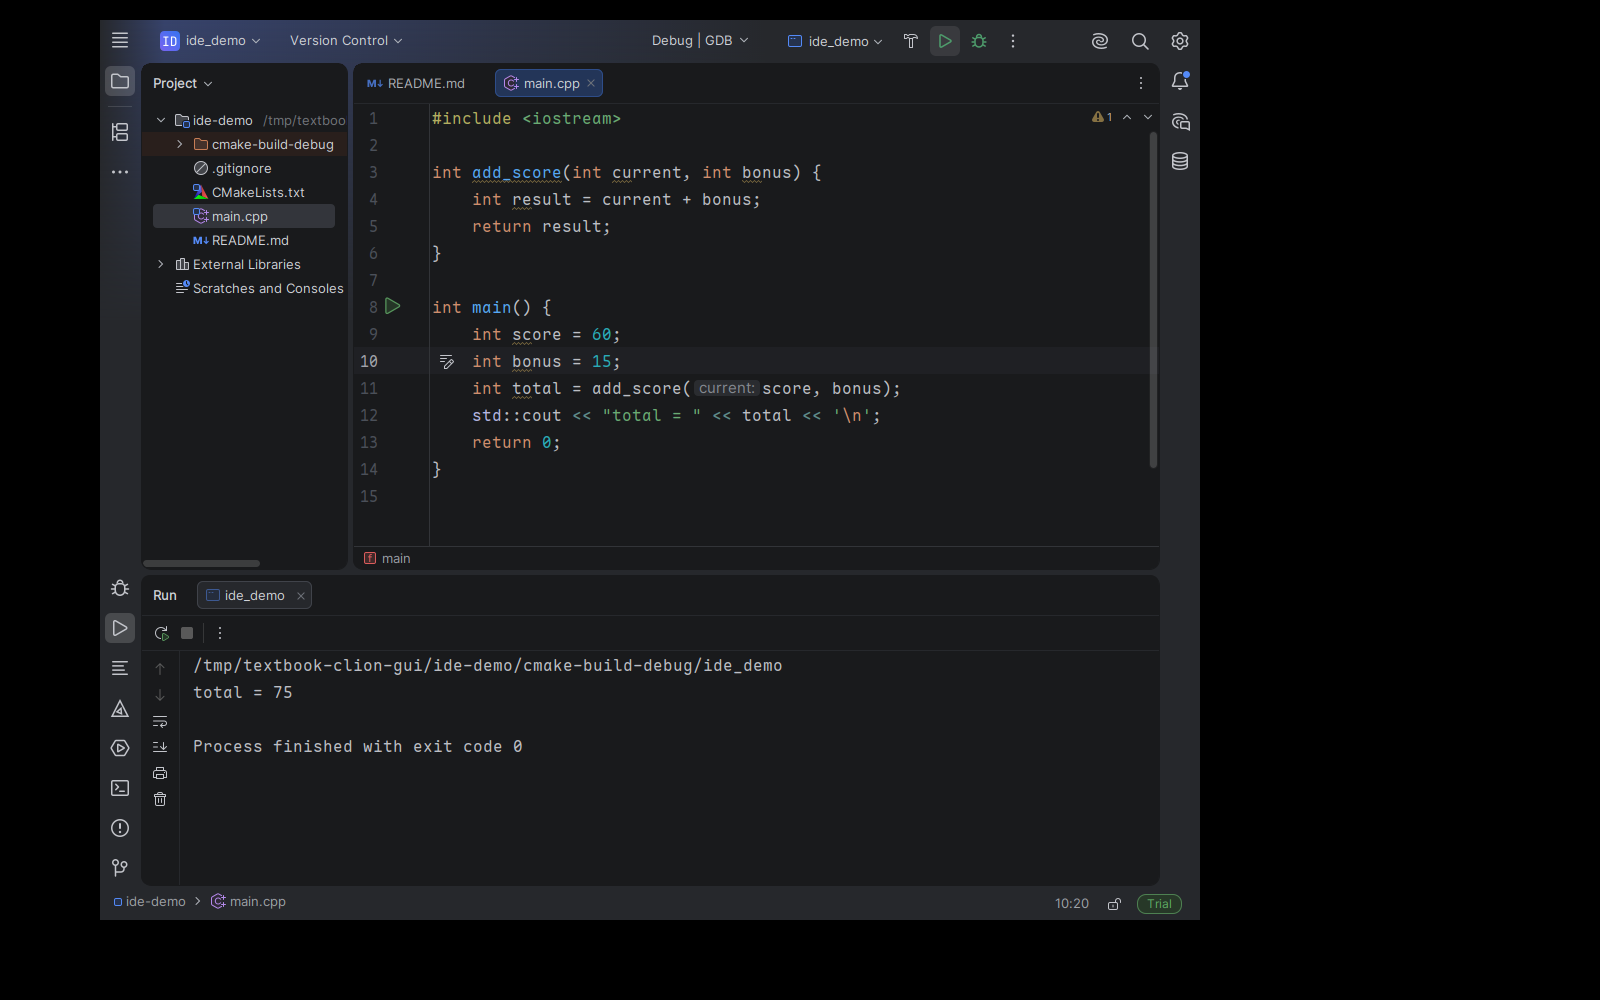
\includegraphics[trim=100bp 220bp 400bp 20bp,clip,width=0.9\textwidth]{ide/clion_run_revised.png}
\caption{CLion 2026.2.3 的界面：左侧工程目录、中央源码、顶部运行控件，底部输出 \texttt{total = 75} 并正常退出}
\label{fig:clion-overview}
\end{figure}

\textbf{先沿窗口边缘找入口，再看中央编辑区。} 下表按位置说明常用按钮；被折叠的工具窗口可从 View → Tool Windows（视图→工具窗口）重新打开。
\begingroup\small
\begin{longtable}{p{0.30\textwidth}p{0.60\textwidth}}
\toprule[1.5pt]
位置／按钮 & 点击后的功能与使用时机\\
\midrule[1pt]\endhead
左上角三横线主菜单 & 展开 File、Edit、View、Navigate、Code、Refactor、Build、Run、Tools、Git、Window、Help；打开项目、设置与退出从这里找。\\
顶部项目名下拉 & 切换或打开项目；先看名称，避免在别的工程中运行。\\
顶部 Git 分支名 & 查看、切换和新建分支；提交前核对分支。未启用 Git 时可能不显示。\\
顶部 Debug／Release 下拉 & 选择 CMake 配置；初学调试选 Debug。新版显示为 Debug | GDB，同时指出所选调试配置。构建参数和构建目录仍在 CMake 设置中检查。\\
顶部目标名下拉 & 选择运行目标；Edit Configurations（编辑配置）设置参数、环境变量、工作目录。\\
锤子 Build（构建） & 编译并链接所选目标，成功后生成程序；只构建不会执行程序。\\
三角 Run（运行） & 通常先构建再运行当前目标，在 Run 窗口看输出；普通运行不在断点暂停。\\
小虫 Debug（调试） & 带调试器启动目标，可在断点暂停并观察变量。\\
方块 Stop（停止） & 终止当前运行或调试进程；仅有活动进程时可用。\\
放大镜 Search Everywhere & 查找文件、符号和动作；连按两次 Shift 也能打开。\\
齿轮 Settings（设置） & 配置字体、快捷键、工具链等；注意区分全局设置与工程设置。\\
右侧铃铛 Notifications（通知） & 查看后台任务、更新和错误提示；读清内容再处理，通知不是编译结果的替代品。\\
顶部 AI／协作图标（若启用） & AI 入口提供代码辅助，Code With Me 等协作入口用于共享会话；本节的本机构建和调试不依赖它们。\\
窗口最小化／最大化／关闭 & 控制整个应用窗口；不同于关闭一个编辑标签或隐藏一个工具面板。\\
\bottomrule[1.5pt]
\end{longtable}\endgroup

\begingroup\small
\begin{longtable}{p{0.30\textwidth}p{0.60\textwidth}}
\toprule[1.5pt]
位置／按钮 & 点击后的功能与使用时机\\
\midrule[1pt]\endhead
左侧文件夹 Project（项目） & 展开目录；双击文件打开；右键目录→New 新建文件，右键文件→Refactor → Rename 重命名并更新引用。\\
左侧 Structure（结构） & 列出当前文件的函数、类等符号，点击可跳转。\\
编辑区顶部文件标签及叉号 & 切换／关闭文件；关闭标签不会删除磁盘文件。CLion 有自动保存机制，运行前仍可按 Ctrl+S 明确保存。\\
行号旁空白槽 & 单击添加／取消红色断点；右键断点可加条件。主函数旁的绿色三角可为相应目标运行或调试。\\
代码旁灯泡／波浪线 & 查看检查结果与建议修复；Alt+Enter 展开动作，先读说明再应用。\\
右侧滚动条标记 & 定位错误、警告和搜索命中；悬停查看提示，点击跳到相应位置。\\
CMake 工具窗口 & 查看配置与生成日志；Reload CMake Project（重新加载）重新读取构建描述，不等于编译。\\
Build（构建）窗口 & 查编译器、链接器输出；点击报错中的文件与行号跳转。\\
Run（运行）窗口 & 看程序输出与退出码；程序等待标准输入时，点击控制台输入。\\
Debug（调试）窗口 & 看调用栈、局部变量、监视表达式与单步控制，详见后面的调试表。\\
Terminal（终端） & 打开当前机器的 shell；Windows 默认终端不因此变成 Ubuntu。\\
Git／Commit 工具窗口 & 查看差异、选择提交文件、写提交说明；提交到本地与推送到远程是两步。\\
工具窗口的省略号／隐藏按钮 & 省略号管理该面板的选项与布局；隐藏只收起面板，不代表停止进程。\\
底部状态栏 & 行列号用于定位，UTF-8 是编码，LF/CRLF 是换行格式，缩进项控制空格／Tab。点击可调整，勿为消除提示随意改全文件。\\
\bottomrule[1.5pt]
\end{longtable}\endgroup

\subsubsection{在 CLion 中构建、运行和调试}
\begin{figure}[H]
\centering
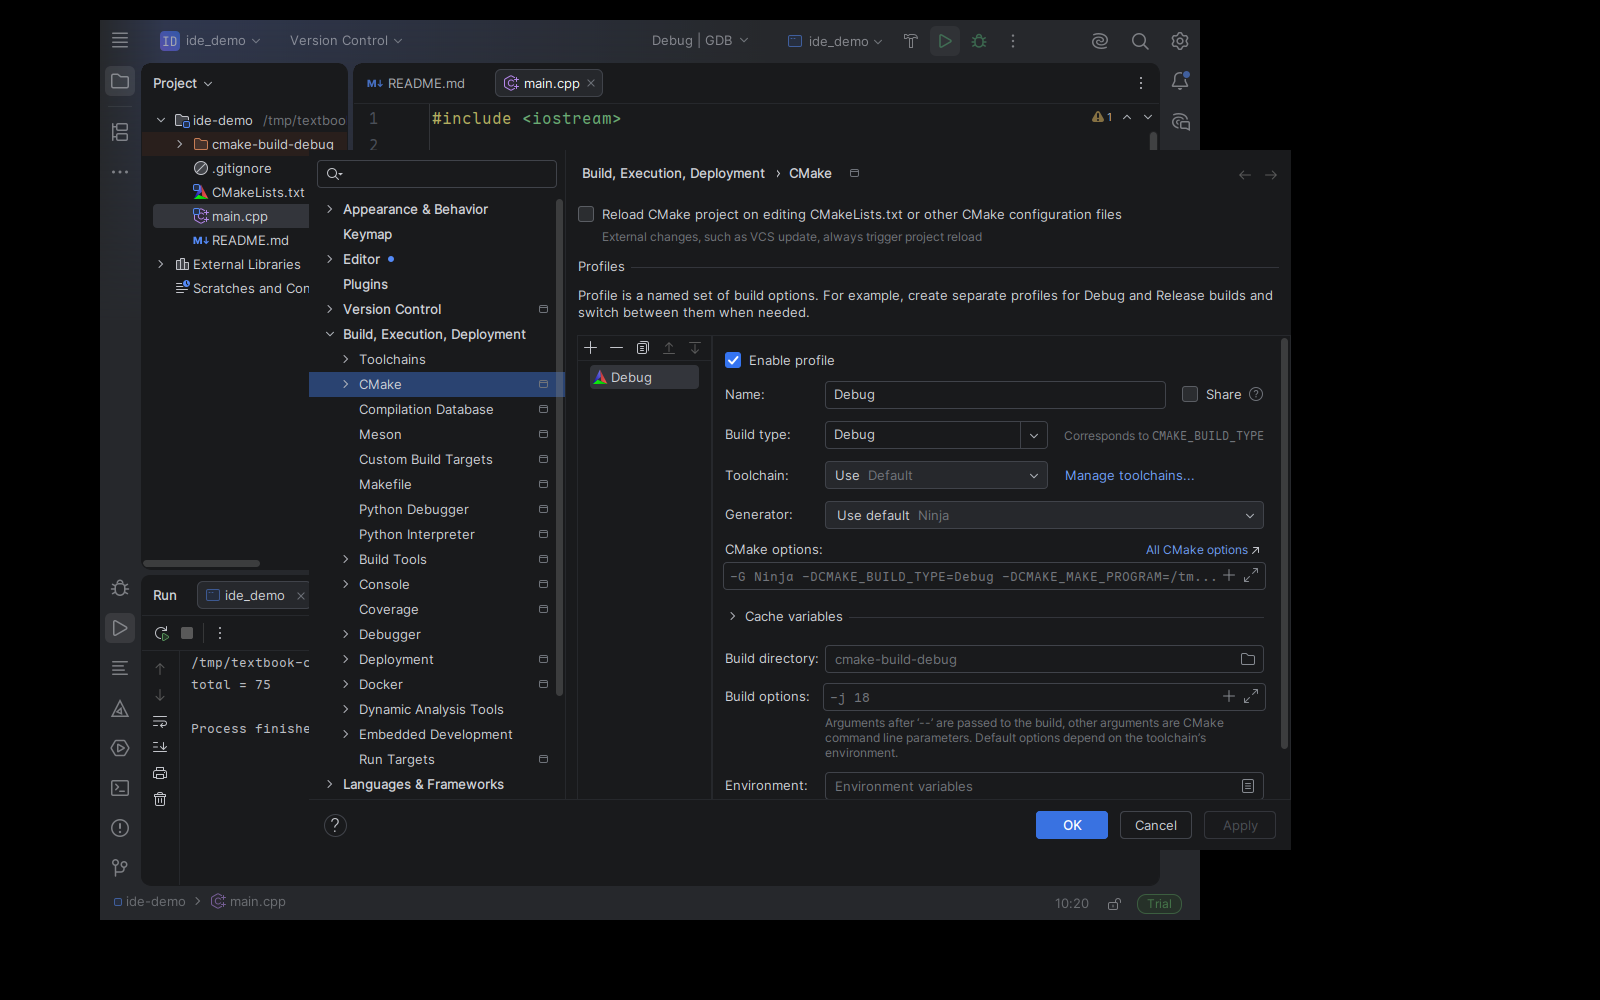
\includegraphics[trim=309bp 150bp 309bp 150bp,clip,width=0.9\textwidth]{ide/clion_cmake_revised.png}
\caption{CMake 设置：Debug 构建类型、默认本机工具链、Ninja 生成器，以及独立的 \texttt{cmake-build-debug} 目录}
\label{fig:clion-cmake}
\end{figure}
\Needspace{8\baselineskip}
\begin{example}
\begin{enumerate}
\item 用 Open 打开练习目录。若出现 CMake 向导，选 Debug、已检测成功的工具链和默认构建目录；等待配置完成。
\item 在顶部选择 \texttt{ide\_demo}，点锤子。Build 窗口应显示成功；再点绿色三角，Run 窗口应出现 \texttt{total = 75} 和退出码 0。
\item 打开 \texttt{main.cpp}，在第 11 行（调用 \texttt{add\_score}）左侧放断点，点小虫。程序暂停时该行\textbf{还没有执行}，所以此时不要读取尚未完成初始化的 \texttt{total}。
\item 在变量区确认 \texttt{score=60}、\texttt{bonus=15}。点 Step Into（步入）进入函数，查看形参 \texttt{current} 和 \texttt{bonus}；单步执行加法，再看 \texttt{result=75}。
\item 点 Step Out（步出）返回调用者，必要时再单步到下一条语句，确认 \texttt{total=75}；点 Resume（继续）直到输出并正常结束。
\end{enumerate}
\end{example}

如果打开工程后直接进入主界面，没有出现向导，我们就从 Settings → Build, Execution, Deployment → CMake 检查图中的配置。名字为 Debug 的配置还要核对 Build type 也确实是 Debug，然后等 CMake 配置完成，再点锤子构建。新版本可能把重新调试做成带回转箭头的小虫；程序还在运行时会先询问是否 Stop and Rerun（停止并重新运行），确认后才会启动新的进程。

运行参数位于目标下拉→Edit Configurations。本例不用参数，工作目录设为工程目录即可；以后程序使用相对路径读图片时，这个目录决定从哪里找文件。
设置里的 Toolchains 选择“用哪些工具”，CMake 配置选择“怎样构建”，运行配置选择“启动哪个程序、传什么参数”。三个入口各管一层。

\begin{exercise}\label{ex:ide-clion}
在 CLion 中将 \texttt{bonus} 改成 20，预测输出，再构建运行验证。在函数内部设置断点，记录执行加法前后的变量值，最后恢复为 15。
\end{exercise}

\Needspace{10\baselineskip}
\section{用 VS Code 开发}
\label{sec:ide-vscode}
\subsubsection{安装 VS Code 与 C++ 扩展}
\paragraph*{Windows 安装步骤}
\begin{enumerate}
\item 从 VS Code 官网下载对应架构的 Windows User Installer。运行后选择安装目录，按需勾选桌面快捷方式、右键“通过 Code 打开”与“添加到 PATH”。安装结束后重新打开终端，PATH 才会在新终端中生效。
\item 启动 VS Code，左侧点四个方块的 Extensions（扩展），搜索并核对发布者 Microsoft，安装 \textbf{C/C++}（\texttt{ms-vscode.cpptools}）和 \textbf{CMake Tools}（\texttt{ms-vscode.cmake-tools}）。二者分别提供 C++ 语言／调试支持和 CMake 工程操作。
\item 如需中文，安装 Microsoft 的 Chinese (Simplified) Language Pack，在命令面板中执行 Configure Display Language，选简体中文并重启。
\item 安装 C++ 编译工具。Windows 本节采用 MSYS2：从其官网安装到默认 \texttt{C:/msys64}，打开 \textbf{MSYS2 UCRT64} 终端，先执行 \texttt{pacman -Suy} 完整更新。若更新提示关闭终端，按提示退出所有 MSYS2 终端，重新打开 UCRT64 后再执行同一命令，直到没有待更新的软件包。然后运行下面的安装命令；遇到包组选择可回车使用默认项，再按提示确认安装。
\end{enumerate}


\Needspace{6\baselineskip}
\begin{tbash}
pacman -S --needed mingw-w64-ucrt-x86_64-toolchain
pacman -S --needed mingw-w64-ucrt-x86_64-cmake mingw-w64-ucrt-x86_64-ninja
\end{tbash}


在 Windows“编辑账户的环境变量”中编辑用户 Path，新增 \texttt{C:\textbackslash msys64\textbackslash ucrt64\textbackslash bin}（自定义安装则换成实际路径）。完全退出并重新打开 VS Code，在新 PowerShell 终端运行 \texttt{g++ --version}、\texttt{gdb --version}、\texttt{cmake --version}、\texttt{ninja --version}，应分别得到版本号。
若有多套工具链，用 \texttt{where.exe g++} 和 \texttt{where.exe gdb} 检查搜索顺序，随后在 CMake Tools 中选择 UCRT64 编译器作为 Kit。CMake Tools 会自动检测直接调试所用的调试器；若调试失败，再检查 GDB 是否来自同一套 UCRT64。

\paragraph*{Ubuntu 安装步骤}
从官网选择 Linux 的 \texttt{.deb} 安装包，架构与机器一致。在下载目录执行 \texttt{sudo apt install ./实际下载的文件名.deb}；这里要替换为真实文件名，不要原样照抄。
编译工具使用前面 Ubuntu 示例的安装命令。启动 VS Code 后同样安装 C/C++ 和 CMake Tools，工具链选系统 GCC。
\begin{note}
VS Code 本体及 C/C++ 扩展\textbf{不包含 C++ 编译器}。先确认版本命令能运行，再处理编辑器配置。
安装参考：\par{\footnotesize\url{https://code.visualstudio.com/docs/setup/windows}\par
\url{https://code.visualstudio.com/docs/setup/linux}\par}
Windows GCC 配置：\par{\footnotesize\url{https://code.visualstudio.com/docs/cpp/config-mingw}\par}
MSYS2 下载：\url{https://www.msys2.org/}。
\end{note}

\subsubsection{VS Code 主界面：活动栏、编辑器和底部面板}
\begin{figure}[H]
\centering
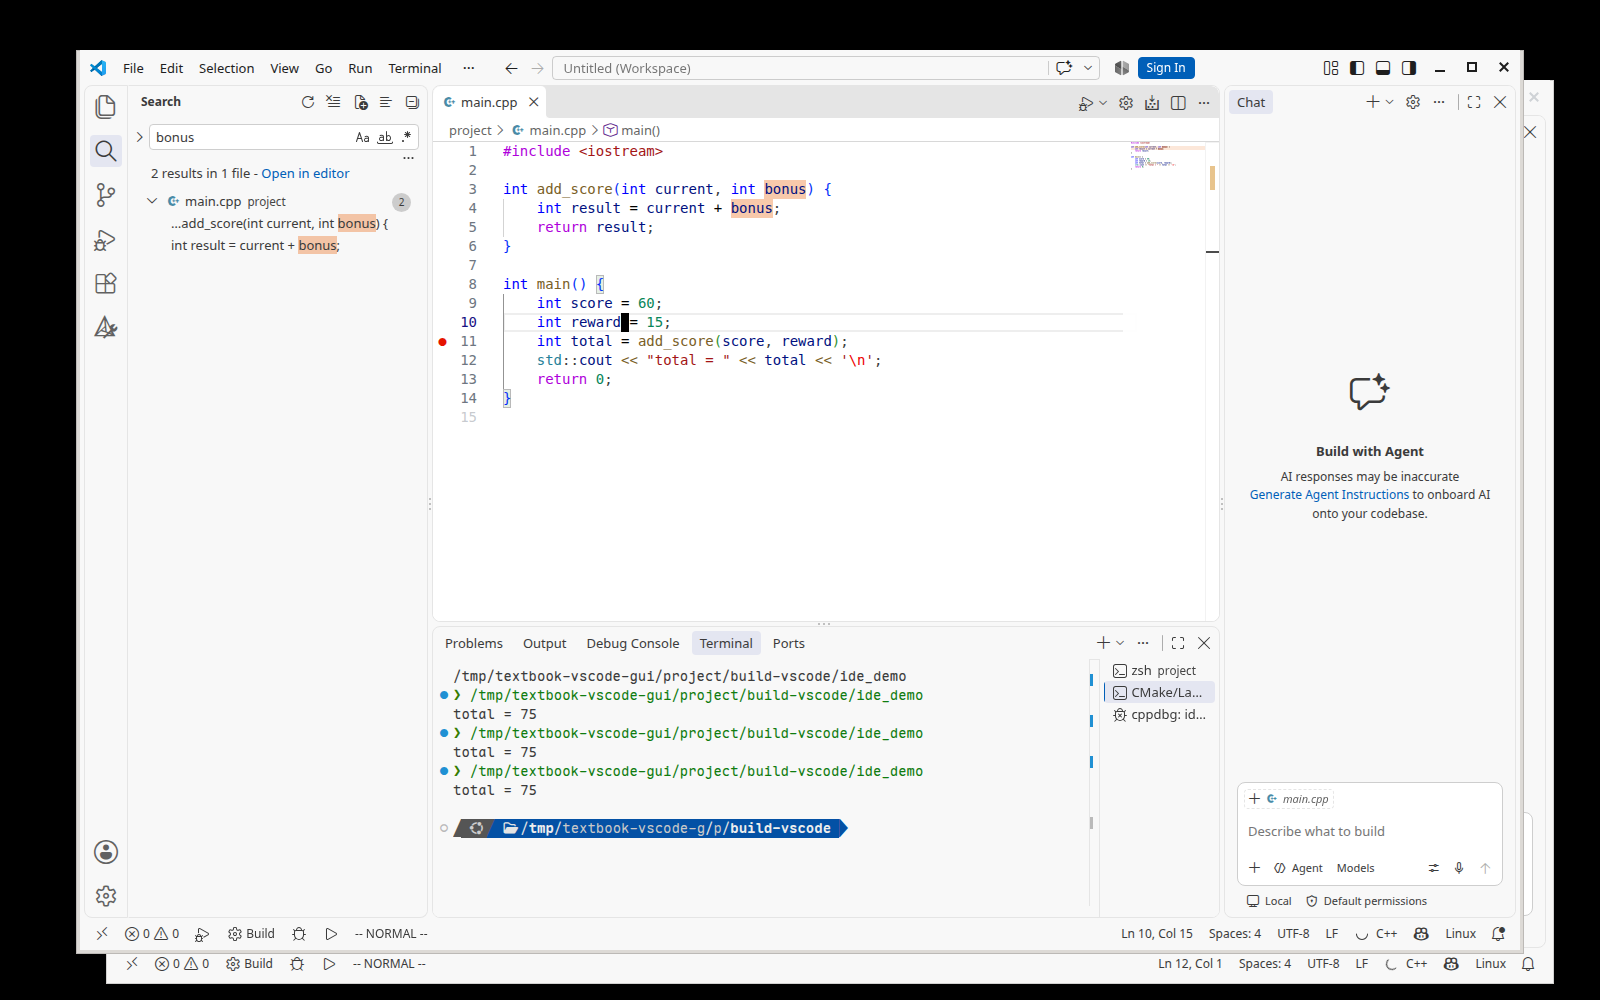
\includegraphics[trim=76bp 46bp 379bp 50bp,clip,width=0.9\textwidth]{ide/vscode_run_revised.png}
\caption{VS Code 1.139.1 的界面：搜索区、编辑区和集成终端；图中已经完成后面的重命名练习，\texttt{main} 中的变量改名为 \texttt{reward}，运行输出为 75}
\label{fig:vscode-overview}
\end{figure}

\begingroup\small
\begin{longtable}{p{0.30\textwidth}p{0.60\textwidth}}
\toprule[1.5pt]
位置／按钮 & 点击后的功能与使用时机\\
\midrule[1pt]\endhead
顶部 File／Edit／Selection & 文件菜单管理打开、保存；编辑菜单提供撤销、查找与替换；选择菜单提供多光标等选择操作。\\
顶部 View／Go／Run & 视图菜单显示面板与命令面板；转到菜单定位文件、行和定义；运行菜单管理调试。窄窗口可能折进省略号。\\
顶部 Terminal／Help & 终端菜单新建终端、运行任务；帮助菜单查看版本、文档和快捷键。\\
顶部搜索框／命令中心 & 快速打开文件、查找命令；Ctrl+P 搜索文件，Ctrl+Shift+P 打开命令面板。\\
左侧纸张 Explorer（资源管理器） & 显示文件树。悬停目录标题出现新建文件、新建文件夹、刷新和折叠全部按钮；双击文件固定标签，单击常为预览。\\
左侧放大镜 Search（搜索） & 跨文件搜索；展开替换框可批量替换。Aa 区分大小写，整词按钮限制完整单词，.* 启用正则表达式。\\
左侧分支 Source Control（源代码管理） & 查看差异；文件旁加号暂存，暂存区减号取消暂存，提交按钮创建本地提交。同步／推送会访问远程。\\
左侧三角加小虫 Run and Debug & 选择调试配置，查看变量、监视、调用堆栈和断点；单击大运行按钮可能要求先配置调试器。\\
左侧四方块 Extensions（扩展） & 搜索、安装、禁用或卸载扩展；齿轮管理某个扩展，核对发布者后再安装。\\
左侧 CMake 图标（安装扩展后） & 展开项目状态与项目大纲，选择工具链、配置、构建目标、启动目标并运行／调试。\\
左下角头像／齿轮 Manage & 头像用于账户相关功能；齿轮打开设置、快捷键、主题等。设置里区分 User（用户）和 Workspace（工作区）作用范围。\\
标题栏布局按钮 & 显示或隐藏主侧栏、底部面板、辅助侧栏等；隐藏侧栏不会关闭工程。\\
额外的活动栏图标 & Python、远程开发、AI 等扩展会增加入口；悬停看名称，用活动栏右键菜单管理显示项。\\
编辑标签、圆点和叉号 & 标签切换文件；圆点表示有未保存修改，Ctrl+S 保存；叉号关闭标签，不删除文件。\\
编辑区右上分栏／省略号 & 分栏可并排查看两个文件；省略号包含当前编辑器的更多动作。\\
编辑区右上三角及下拉 & 含义由语言与扩展决定，可能是运行当前文件；CMake 工程按后文的 CMake 命令运行整个目标。\\
面包屑／缩略图 & 面包屑显示文件路径与函数层级，点击定位；右侧缩略图帮助快速滚动长文件。\\
行号左侧与折叠箭头 & 点空白槽设断点；点折叠箭头收起代码块，不会删除代码。\\
Problems（问题） & 汇总诊断；点某条跳转到对应行，错误计数不等于本次构建一定失败，须结合构建日志判断。\\
Output（输出） & 看扩展日志，右侧下拉选择 CMake 等通道；通常不能在这里给程序输入。\\
Debug Console（调试控制台） & 看调试信息、求表达式值；C++ 程序的标准输入一般使用终端或外部控制台。\\
Terminal（终端） & 运行 shell 命令或与程序交互；加号新建终端，下拉选 PowerShell/Bash 等，分栏并排显示，垃圾桶结束该终端及其会话。\\
面板最大化／叉号 & 最大化扩大面板，叉号隐藏面板；隐藏终端面板不会自动结束里面的程序。\\
底部行列号、Spaces、UTF-8、CRLF/LF & 分别控制定位、缩进、编码和换行格式；C++ 表示当前语言模式，若误为 Plain Text，应改为 C++。\\
底部错误／警告、分支、远程标记 & 点计数打开问题；分支项处理版本控制；远程标记用于连接 WSL/SSH 等环境。先确认当前到底连在哪台机器。\\
\bottomrule[1.5pt]
\end{longtable}\endgroup

接下来用同一个计分器练习。配置或构建报错时，到 Output 的 CMake 通道看日志。程序启动后，再到 Terminal 核对实际输出。

\Needspace{10\baselineskip}
\subsubsection{在 VS Code 中运行同一个 CMake 工程}
\Needspace{8\baselineskip}
\begin{example}
\begin{enumerate}
\item File → Open Folder 打开练习目录。检查文件树顶层的两个文件。自己创建或已检查的教材工程可按提示信任；未知工程先在受限模式下检查内容。
\item 按 Ctrl+Shift+P 打开命令面板，输入 \texttt{CMake: Select a Kit}，选实际安装的 GCC：Windows 用 UCRT64，Ubuntu 用系统 GCC。若找不到，先运行 \texttt{CMake: Scan for Kits}。
\item 执行 \texttt{CMake: Select Variant}，选择 Debug；再执行 \texttt{CMake: Configure}。在 Output 中选 CMake 通道，确认配置、生成成功。
\item 执行 \texttt{CMake: Build}，等待成功，再执行 \texttt{CMake: Run Without Debugging}。若询问启动目标，选择 \texttt{ide\_demo}；终端应输出 \texttt{total = 75}。
\item 在第 11 行左侧点出红色断点，执行 \texttt{CMake: Debug}，观察程序停在该行。按后面表格单步并检查变量，再继续到退出。
\end{enumerate}
\end{example}

本例没有 CMake Presets，因而使用 Kit（工具链组合）与 Variant（构建类型）路线。
如果工作区启用了 Presets，命令可能变成 Select Configure Preset；先在工作区设置中将 \texttt{cmake.useCMakePresets} 设为 \texttt{never} 再做本例。
以后接手带 \texttt{CMakePresets.json} 的队内工程时，应使用工程提供的预设。
CMake Tools 的按钮可能在侧栏 Project Status，也可能在底部；\textbf{上述命令面板是布局变化时的备用入口}。
不过，输入动作名后先核对列表里的完整名字，再按回车：最近使用过的动作和相似名字可能排在前面。
例如 \texttt{CMake: Build} 是构建，\texttt{Append Build Directory to Current Workspace} 则是把构建目录加入工作区；名字里都有 Build，做的事情却不同。
若需要显式指定构建目录，可在工作区设置搜索 \texttt{cmake.buildDirectory}，使用 \texttt{\$\{workspaceFolder\}/build-vscode}。

\begin{note}
本例用 CMake Tools 直接启动调试，不要求手写 \texttt{launch.json}。
以后需要自定义时，\texttt{tasks.json} 描述任务，\texttt{launch.json} 描述如何启动调试，\texttt{c\_cpp\_properties.json} 配置代码分析；它们都不代替 \texttt{CMakeLists.txt}。
代码补全无红线只能说明分析器接受配置，不能证明程序已经编译成功。
\end{note}

\begin{exercise}\label{ex:ide-vscode}
用 VS Code 打开同一练习工程，搜索 \texttt{bonus}，跳转到定义，再将它重命名为 \texttt{reward}（使用 Rename Symbol／重命名符号，而非无差别全文替换）。保存、构建并运行，确认输出仍为 75；最后撤销并保存。
\end{exercise}

\section{单步调试与常见问题}
\label{sec:ide-debug}
\subsubsection{调试工具栏：不要只记小虫和三角}
\begin{figure}[H]
\centering
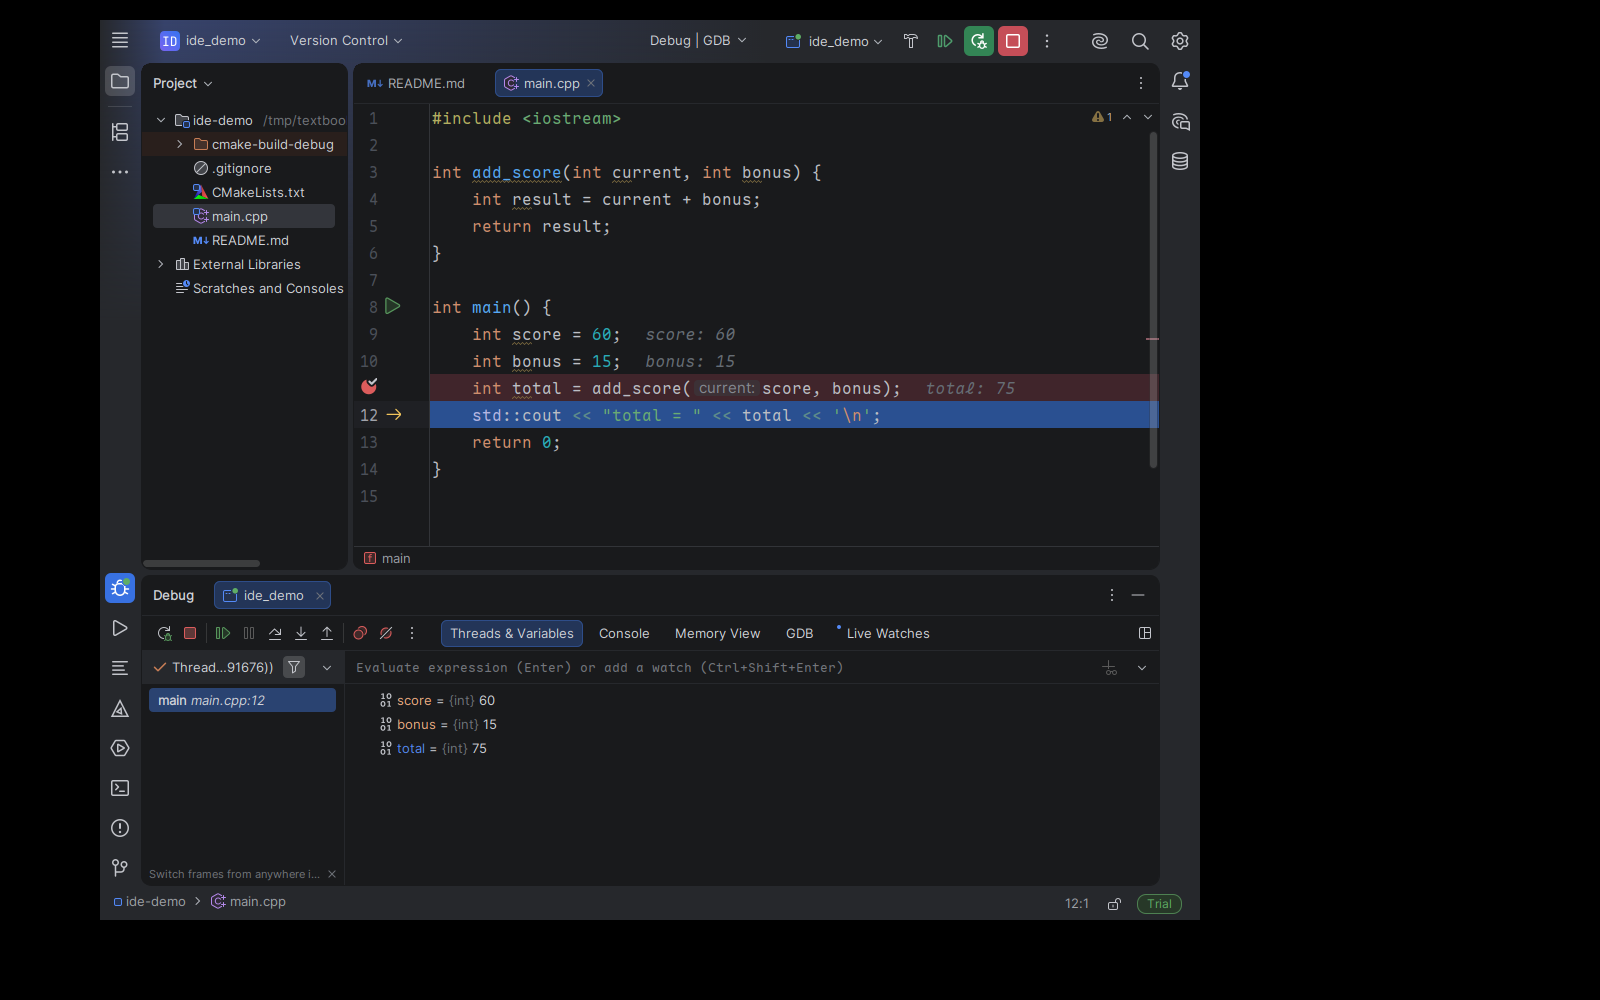
\includegraphics[trim=100bp 220bp 400bp 20bp,clip,width=0.9\textwidth]{ide/clion_debug_revised.png}
\caption{CLion 实际单步后停在第 12 行：第 11 行赋值已完成，变量区显示 \texttt{score=60}、\texttt{bonus=15}、\texttt{total=75}；左侧为调用栈，底部为单步按钮}
\label{fig:clion-debug}
\end{figure}
调试（Debugging）的目标是观察程序如何执行。断点让程序在某行执行前暂停，单步决定下一次停在哪里。
以下快捷键为 Windows/Linux 常见默认键位；若换过 Keymap，以按钮悬停提示为准。
\begingroup\small
\begin{longtable}{p{0.28\textwidth}p{0.14\textwidth}p{0.16\textwidth}p{0.31\textwidth}}
\toprule[1.5pt]
按钮／功能 & CLion & VS Code & 使用时机\\
\midrule[1pt]\endhead
Continue／Resume 继续（三角） & F9 & F5 & 跑到下一断点或程序结束。\\
Pause 暂停（双竖线） & 看工具栏 & F6 & 运行中请求暂停，排查卡在哪里。\\
Step Over 步过（弯箭头） & F8 & F10 & 执行当前行，函数调用整体完成。\\
Step Into 步入（向下箭头） & F7 & F11 & 进入当前行调用的函数内部。\\
Step Out 步出（向上箭头） & Shift+F8 & Shift+F11 & 执行到当前函数返回调用者。\\
Restart／Rerun 重新开始（回转箭头） & 看工具栏 & Ctrl+Shift+F5 & 重新启动进程，不是把时间倒回上一行。\\
Stop 停止（方块） & Ctrl+F2 & Shift+F5 & 结束当前调试会话／启动的程序。\\
Toggle Breakpoint 切换断点 & Ctrl+F8 & F9 & 在当前行添加或取消断点。\\
\bottomrule[1.5pt]
\end{longtable}\endgroup

\begin{figure}[H]
\centering
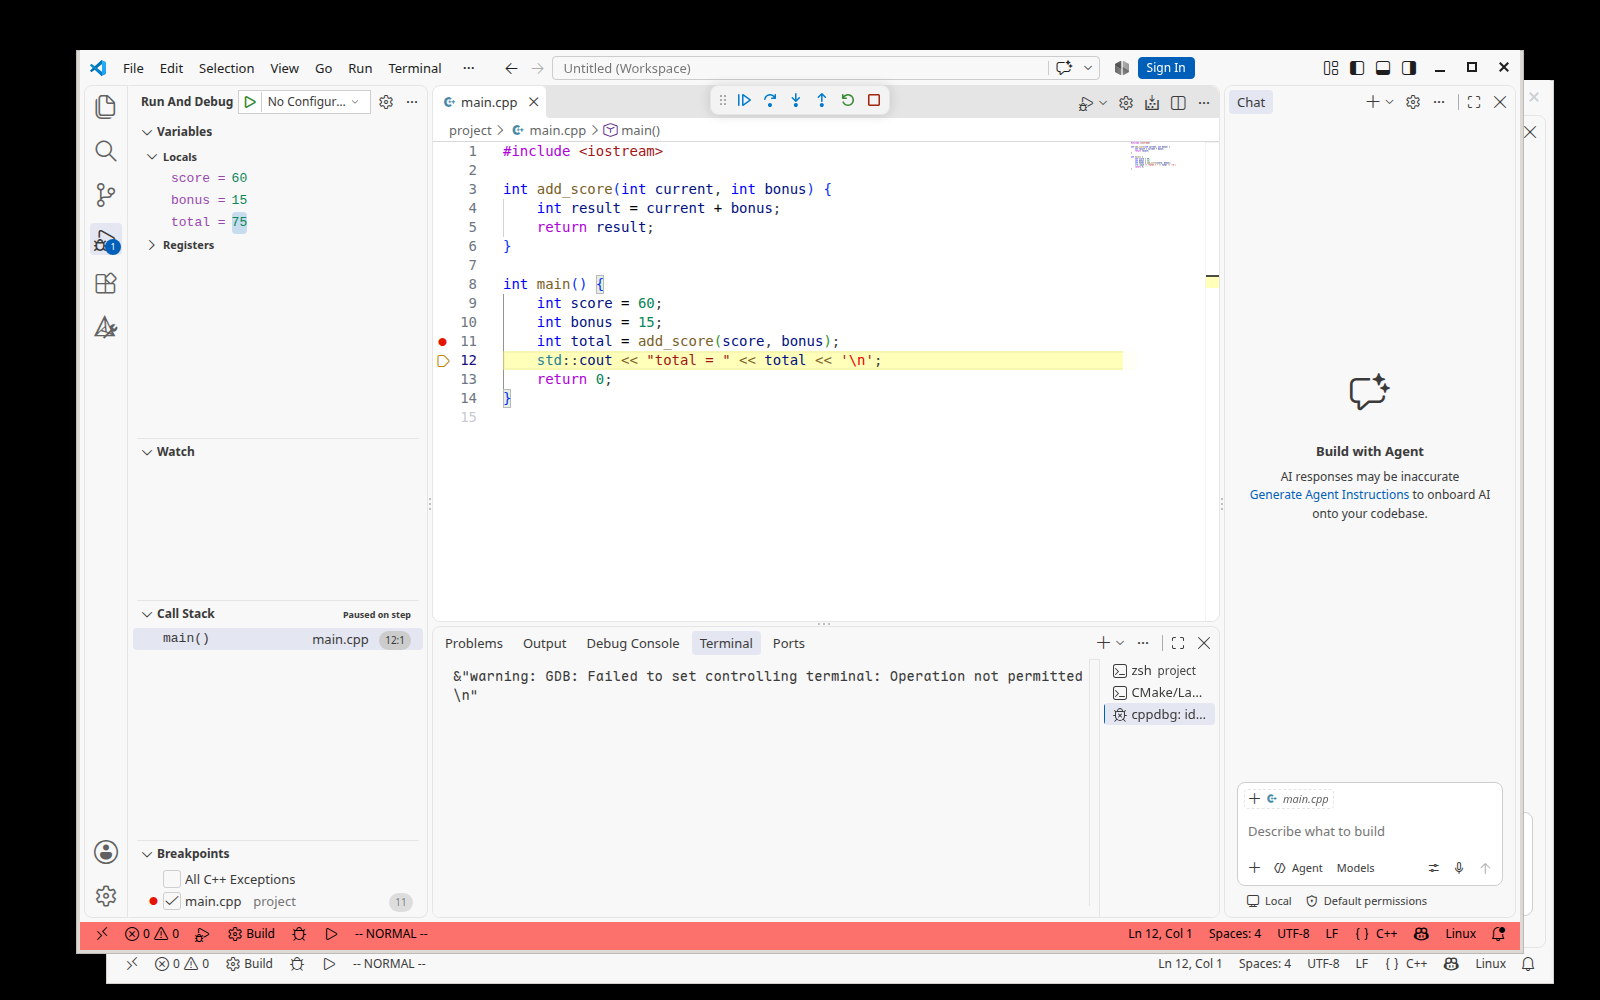
\includegraphics[trim=76bp 375bp 379bp 50bp,clip,width=0.9\textwidth]{ide/vscode_debug_revised.png}
\caption{VsCode 中的实际单步结果：执行第 11 行后停在第 12 行，左侧 \texttt{total = 75}；顶部是调试工具栏}
\label{fig:vscode-debug}
\end{figure}
\textbf{变量（Variables）}显示当前栈帧的局部变量；\textbf{监视（Watches/Watch）}可以添加 \texttt{score + bonus} 等表达式；
\textbf{调用栈（Frames/Call Stack）}显示函数调用关系，点击不同帧会切换变量作用域；\textbf{断点列表（Breakpoints）}集中启用、禁用或移除断点。
表达式必须在当前作用域有效：进入 \texttt{add\_score} 后看形参 \texttt{current}，想查看 \texttt{main} 的 \texttt{score} 则切回它的栈帧。
在暂停状态下查看简单表达式即可；会修改变量或调用函数的表达式可能改变被调试程序。

\begin{conclusion}
\begin{itemize}
\item 保存只把修改写到磁盘；配置读取 CMake 规则；构建生成程序；运行启动程序；调试带着调试器启动程序。
\item Run 不停在断点，Debug 才会；断点高亮行尚未执行，变量也必须已初始化才有可解释的值。
\item 工具链、构建配置、运行配置分开检查；界面布局变了就按动作名搜索，不凭图标颜色猜功能。
\end{itemize}
\end{conclusion}

\subsubsection{常见问题与排查顺序}
\begingroup\small
\begin{longtable}{p{0.29\textwidth}p{0.61\textwidth}}
\toprule[1.5pt]
现象 & 先检查什么\\
\midrule[1pt]\endhead
找不到编译器或 CMake & 在当前环境的终端查版本和路径；安装后重启 IDE。CLion 检查 Toolchains，VS Code 检查 Kit，不能只安装扩展。\\
运行按钮灰色／没有目标 & 是否打开了含 CMakeLists.txt 的目录？CMake 配置是否成功？该文件中是否创建了可执行目标？\\
修改了代码但输出不变 & 保存文件，检查当前工程、构建目录和启动目标，再构建运行，避免运行另一份旧程序。\\
断点空心／不停／变量被优化 & 使用 Debug 构建并启动调试；确认正在运行刚构建的程序，断点所在代码确实会执行。\\
更换工具链后 CMake 报缓存冲突 & 为新工具链换一个构建目录并重新配置；不要让 MSVC、MinGW、Linux 共用缓存。\\
终端有输出却不能输入 & 确认是 Terminal/Run 控制台，且程序还活着并在读输入；Output 只是日志。本例输出后立即退出。\\
编辑器红线与构建结果不一致 & 检查 C++ 扩展的编译器路径、标准与 CMake 配置提供者，再查看真实构建日志。\\
Windows 能跑，Ubuntu 找不到文件 & 检查路径大小写、斜杠、工作目录和系统依赖；不要复制 Windows 可执行文件到 Ubuntu 当作本机程序。\\
\bottomrule[1.5pt]
\end{longtable}\endgroup

\begin{exercise}\label{ex:ide-setup}
按所选工具完成练习~\ref{ex:ide-clion} 或~\ref{ex:ide-vscode}，再记录当前系统、编译器路径、Debug 构建目录和一次运行的退出码。在界面中指出终端、构建日志、运行输出和变量窗口。以后换工具时，用同一份记录对照。
\end{exercise}

\begin{exercise}\label{ex:ide-debug}
在第 11 行的函数调用前暂停，先预测步入后最先能看到的参数和值。步入后查看当前栈帧，再步出并单步到第 12 行，核对 \texttt{total}。如果断点未命中，说明会怎样检查构建类型和正在调试的目标。
\end{exercise}

\begin{note}
界面与操作核对资料：
\par\footnotesize
\url{https://www.jetbrains.com/help/clion/guided-tour-around-the-user-interface.html}\par
\url{https://www.jetbrains.com/help/clion/debugging-code.html}\par
\url{https://www.jetbrains.com/help/clion/configuring-debugger-options.html}\par
\url{https://code.visualstudio.com/docs/getstarted/userinterface}\par
\url{https://code.visualstudio.com/docs/cpp/cmake-linux}\par
\url{https://code.visualstudio.com/docs/debugtest/debugging}
\end{note}
\endgroup

\section{终端开发环境：AstroNvim*}
\label{sec:astronvim-customize}

Vim 本身有语法高亮与基础补全，但插件组合需要配置。Neovim（nvim）是 vim 的现代化分支，而 AstroNvim 是一套开箱即用的 Neovim 配置——装完就有文件树、模糊搜索、代码补全和漂亮的界面，毛坯房直接变精装，终端里也能有接近 IDE 的体验。

\textbf{安装新版 Neovim}

AstroNvim 需要较新版本的 Neovim，而 Ubuntu 22.04 仓库自带的版本太老，因此先核对官方要求再安装。下面仅用于 \texttt{x86\_64}，如果是在 Nvidia Orin NX 等 ARM 机器安装需要换用 arm64 架构包：

\Needspace{8\baselineskip}
\begin{example}
下载并解压 Neovim 到 \texttt{/opt}，顺手装上两个依赖（ripgrep 用于全局搜索，gcc 用于编译语法高亮组件）：


\Needspace{8\baselineskip}
\begin{tbash}
curl -fLO https://github.com/neovim/neovim/releases/latest/download/nvim-linux-x86_64.tar.gz
sudo tar -C /opt -xzf nvim-linux-x86_64.tar.gz
sudo apt install ripgrep gcc
\end{tbash}


然后把刚刚解压出的 bin 目录放到 PATH 前面，这样 Shell 会优先找到新版 Neovim。下面的设置只对当前会话生效；想长期使用，可以把这一行写入自己的 Bash 或 zsh 配置，方法见卷一第 1 章《Shell 脚本与环境变量》一节：


\Needspace{5\baselineskip}
\begin{tbash}
export PATH=/opt/nvim-linux-x86_64/bin:$PATH
\end{tbash}


生效后执行 \texttt{command -v nvim} 与 \texttt{nvim --version}，确认找到的是新安装的程序且版本满足要求；若旧版抢先被找到，把新目录放到 PATH 前面。
\end{example}

\textbf{安装 AstroNvim}

先用独立配置试用 AstroNvim。这里用 \texttt{NVIM\_APPNAME} 让 Neovim 把本次的配置、数据和缓存放到名为 \texttt{astronvim-training} 的目录下。需要 Git，已有同名练习目录时先换一个名字，并同步修改下面两处。
\href{https://docs.astronvim.com/reference/alt_install/}{官方独立安装说明}还给出了设置常用启动命令的方法。

\begin{example}[用独立配置打开练习工程]
在 Ubuntu 终端中执行以下命令，最后一行在复制好的 \path{ide-demo} 根目录运行。

\begin{tbash}
git clone --depth 1 https://github.com/AstroNvim/template ~/.config/astronvim-training
NVIM_APPNAME=astronvim-training nvim .
\end{tbash}

首次启动会下载插件。等待安装完成，再用空格键打开快捷键菜单，试着搜索 \texttt{main.cpp}。运行普通的 \texttt{nvim} 时会使用你平时的配置。
\end{example}

\begin{figure}[H]
    \centering
    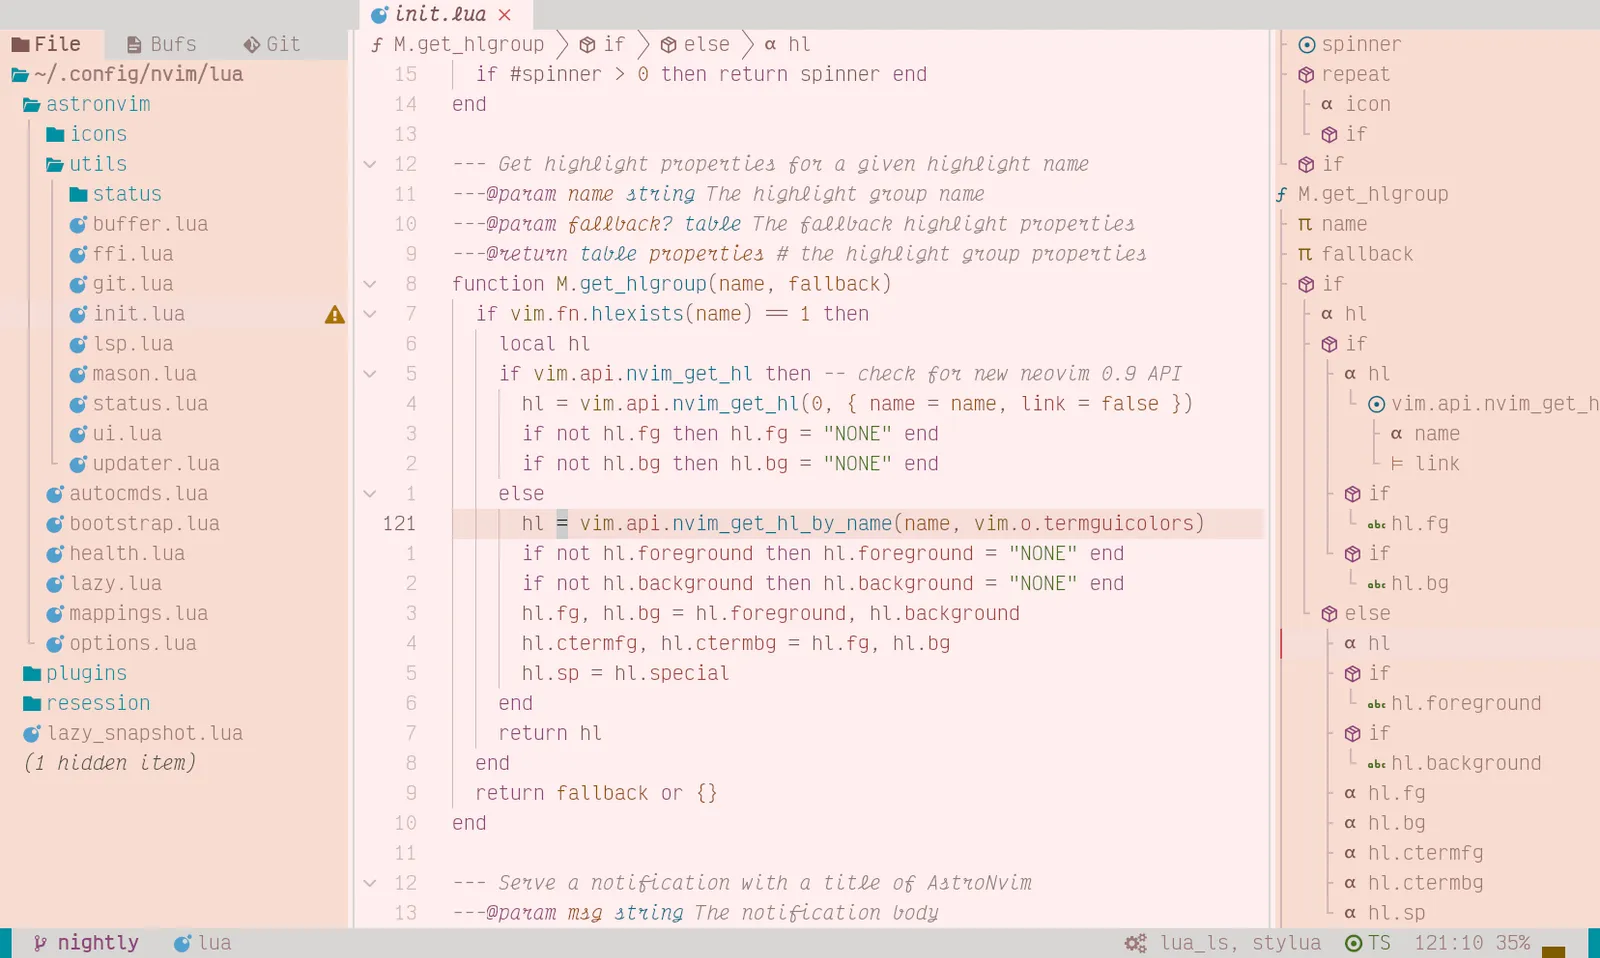
\includegraphics[width=0.8\textwidth]{ide/astronvim_welcome.png}
    \caption{AstroNvim 界面}
    \label{fig:astronvim}
\end{figure}

\textbf{上手要点}

\begin{itemize}
\item Leader 键是空格：按下 \texttt{<Space>} 稍等片刻会弹出快捷键菜单，忘了按键组合也不用背，跟着菜单按就行；
\item \texttt{<Space>ff} 模糊搜索并打开文件，\texttt{<Space>fw} 在整个项目中搜索文字（依赖 ripgrep）；
\item 在 \texttt{:Mason} 中查找并安装 \texttt{clangd}，打开 \texttt{main.cpp} 后用 \texttt{:checkhealth vim.lsp} 核对语言服务器已连接，再试补全和跳转。
\end{itemize}

\begin{note}
界面中的图标和 zsh 的 p10k 主题一样依赖 Nerd Font，装过 MesloLGS NF 的话直接通用（见卷一附录《zsh 与终端美化》）。更多用法见官方文档：\url{https://docs.astronvim.com/}
\end{note}

\begin{exercise}\label{ex:v0-astronvim}
完成 AstroNvim 的安装，用 \texttt{<Space>ff} 打开任意一个文本文件，再用 \texttt{<Space>fw} 在某个项目目录中搜索一个关键词，体验模糊搜索。
\end{exercise}

\section{本章小结}
CLion 和 VS Code 用的是同一条工作流：先确认当前系统和工具链，再打开含 \texttt{CMakeLists.txt} 的目录、配置目标、构建并运行。程序结果与预期不同时，用 Debug 构建停在断点，沿调用栈和变量值逐步核对。换 IDE 时，可以先找这些动作的入口，再熟悉界面布局。习惯终端的同学也可以用 AstroNvim 编辑与导航，并在终端运行 CMake 命令。下一章仍会用到这条工作流：让 AI 协助改代码之后，你要能亲自构建、调试并验证结果。

\begin{problemset}
\item \label{prob:v0-ide-1} （基础）分别说明 CLion 的锤子、绿色三角、小虫按钮的作用，以及 VS Code 的 Explorer、Extensions、Terminal、Output 各负责什么。为什么装好 VS Code 的 C/C++ 扩展后仍可能无法编译？
\item \label{prob:v0-ide-2} （提高）同一份源码先用 Windows 的 MinGW 构建，再用 Ubuntu 中的 GCC 打开。可以沿用同一个 CMake 构建目录吗？如果改了源码却仍看到旧输出，应依次核对什么？
\item \label{prob:v0-ide-3} （实践）在练习副本把 bonus 改为 25，先预测输出，再用一套 IDE 的 Debug 配置构建并验证。在第 11 行步入函数，记录两个参数；回到调用者后观察 total。提交实际构建目录与对应输出。
\end{problemset}

\section{本章验收}
\begin{enumerate}
\item 任选 CLion 或 VS Code 打开教学工程，指出菜单、文件树、编辑区、构建入口、运行入口、调试入口、终端和状态栏，并运行得到 \texttt{total = 75}。
\item 在所选工具中现场断点调试：在函数调用处暂停，演示步入、步过、步出、继续；指出当前栈帧与变量值，并解释为什么暂停行的赋值尚未生效。
\end{enumerate}

进阶练习时，再换另一套工具跑同一份源码，比较工具链选择、独立构建目录和调试入口。

\chapter{用 AI 协作开发}
\label{chap:ai-development}

\begin{introduction}
  \item 学习目标：写清要解决的问题，选择聊天或代码代理，核对改动、权限与实际运行结果。
  \item 建议学时：初读约 1 小时，含计分器练习。工具操作按需查阅，项目实作可另安排 2--3 天。
  \item 学习顺序：初读使用手边的聊天工具。准备在仓库中审查、回退或交付修改时，再做需要 Git 与构建基础的实作。
\end{introduction}

\begingroup
\setlength{\emergencystretch}{3em}
\clubpenalty=10000
\widowpenalty=10000

也许你已经知道 AI 工具，也用它问过概念、改过文字，或者贴过一段报错。现在试着用 AI 帮你改刚跑通的计分器。你告诉它“这一轮扣 5 分”，它可能找到正确的一行，也可能把输出直接写成 55。两种改法这次都能显示 55，你会怎么分辨？

先从第~\ref{sec:ai-first-practice}--\ref{sec:ai-evidence}~节试起。一路练习怎么问、什么时候用聊天或代理，以及怎样确认工具做过什么。完成这条路线后，可到第~\ref{sec:ai-acceptance}~节做入门验收。遇到具体工具问题时查中间的说明，开始改仓库时再做后面的项目练习。

\section{首次上手：先写预期，再验证 AI 的建议}
\label{sec:ai-first-practice}

上章的计分器已经在你的电脑上跑出了 \texttt{total = 75}。现在设想规则变了：基础分仍是 60，这一轮要扣 5 分。AI 可以帮你找到要改的一行。改之前先在纸上算一遍，给自己留一个判断结果的依据。

\begin{example}[请 AI 建议一处小改动]
先复制卷零的 \path{examples/ide-demo}，用上章选好的 IDE 打开副本，并重新构建运行。看到原始结果 75 后，写下新规则下的预期 55。把练习项目的 \texttt{main.cpp} 贴到你手边的 AI 聊天工具，附上下面的要求：

\begin{quote}
这是我刚跑通的计分器，当前输出 total = 75。基础分保持 60，这一轮要扣 5 分。请指出需要改哪一行，解释为什么，并给出改前改后的那一行。保留计分函数和输出格式。
\end{quote}

自己对照原文件，确认改的是 \texttt{main} 中的 bonus 初始化，把 15 改成 \texttt{-5}。如果建议改到了计算函数或写死了输出，先回看任务范围。保存后重新构建和运行，输出应为 \texttt{total = 55}。再亲手把 bonus 改成 0，先预测输出，再重新构建运行，核对是否为 \texttt{total = 60}。如果观察到旧输出，回看第~\ref{sec:ide-debug}~节的构建与启动目标检查。
\end{example}

\begin{conclusion}
AI 的解释是待验证的线索。先写预期，确认实际改动，再用自己的输入重新运行。遇到问题时，把你看到的报错和复现步骤一起交给 AI 或队友。
\end{conclusion}

\begin{exercise}\label{ex:ai-first-practice}
现在基础分仍为 60，改成加 7 分。给 AI 写一条只解释改动、只涉及一行代码的请求。记录自己的预期、AI 建议的位置、实际改动与重新构建后的输出。再自选一个不同的加分值，独立核对一次。
\end{exercise}

\section{提示词：把愿望写成可以验收的任务}
\label{sec:ai-prompts}

刚才请 AI 修改计分器时，我们给了原始输出、新规则和允许改动的范围。换一个问题，你可能会问：“我说得挺清楚，它怎么还是改错了？”先看看你的提示词有没有把\textbf{现象、目标与验收}分开。“优化识别效果”只有方向，没有说明在哪组图上、用什么指标判断、允许付出多少延迟；模型只好替你猜。猜得再流畅，也不等于猜中了队内需求。

给 AI 的请求和材料通常叫提示词（Prompt）。对于开发任务，先用下面几项把问题说清楚，让 AI 拥有充足的上下文。
\begin{center}
\begin{tabular}{p{0.16\textwidth}p{0.73\textwidth}}
\toprule
信息 & 应写出的内容 \\
\midrule
目标与现象 & 现在发生什么，期望变成什么；把“修复卡顿”变成一个可观察行为。\\
相关证据 & 仓库、入口文件、复现命令、完整的相关报错、输入样本与版本。\\
范围与约束 & 哪个模块可修改，接口、单位、依赖与硬件条件有什么限制。\\
验收与交付 & 用什么命令、样本和指标判断完成；交付代码、说明还是方案。\\
不确定处 & 哪些条件还不知道，先调查什么，哪些决策需要向你确认。\\
\bottomrule
\end{tabular}
\end{center}

但也不要为了凑“上下文”粘贴几万行日志。给出首次错误附近的日志、运行命令及文件路径，让有工具的代理自行定位其余内容；未获本地文件访问能力的聊天需要你附上最小相关代码或文件。截图适合表达界面、曲线与视觉现象，编译错误优先附可复制的文本。发送前检查日志与附件，移除令牌、密码、队友隐私和无关的队内资料。

\begin{example}[同一个错误，怎样从许愿变成任务]
假设你在计分器里把 bonus 改成了 -5，运行时却仍看到 75。与其只说“帮我修一下”，可以先这样请 AI 帮你排查：
\begin{quote}
我在计分器的 \texttt{main.cpp} 中把 bonus 从 15 改成了 -5。基础分是 60，预期输出 55，但点运行仍显示 75。我还没确认这次启动的是不是新构建的目标。请先指出最值得核对的两步，并说明每步要看什么。先给检查办法，保留计分函数。
\end{quote}
这个提问给出了预期和观察结果，也说清了尚未确认的条件。你可以先看构建日志是否显示编译成功，再检查 IDE 实际启动的目标与构建目录。若仍找不到原因，补上相关日志和路径，把调查缩小到能复现的那一步。拿到建议后，用实际结果排除原因。
\end{example}

反馈也要有证据。不要反复发送“还是不行”“再聪明一点”；写清“新构建后输入为……，实际输出……，预期……，这是命令和日志”。如果你怀疑它的方案，要求它比较候选原因、列出能区分这些原因的实验，或指出结论对应的文件与官方资料。\textbf{要让 AI 给出可检查的解释与依据}，不能把 AI 的幻觉当成事实，更不能把一大段解释当成验证。

代理运行时，发现关键约束漏了就及时补充；下一项独立任务可以排队。不要一边让它修函数，一边在同一聊天中突然讨论装系统。若目标已经变了，要明确说“停止当前任务，保存现状，改做……”，并检查仍在运行的命令。功能入口见第~\ref{sec:ai-workflow}~节。

\begin{exercise}\label{ex:ai-prompt}
用自己遇到的一个构建或运行问题练习。如果手边刚好没有错误，可在计分器练习副本删掉一处分号，重新构建并记录第一条相关报错。写一条让 AI 先给检查建议的请求，说明操作步骤、预期、实际现象、相关代码和判断是否恢复的办法。修复后记录实际结果。
\end{exercise}

\section{先选工作方式，再选工具}
\label{sec:ai-entry}

\textbf{普通聊天}适合问概念、比较思路、讨论需求，或针对一小段代码请它逐步讲解；这时你主要阅读回答，再决定下一步。需要查资料、读取实验记录、分析数据并制作报告时，可以选择支持\textbf{多步骤工具任务}的工作方式，让 AI 调用工具、读取结果后继续处理。需要进入源码工程，搜索文件、修改代码、执行命令并读取报错时，则适合具备相应工具的\textbf{代码代理（Coding Agent）}。代码代理的价值来自“查看工程—采取行动—验证结果”的循环，而不只是一次生成更长的回答。

这些工作方式没有绝对互斥的边界。同一产品可以在聊天中启用搜索、文件或代码工具，代码代理也能只讨论而不修改。判断时应查看\textbf{当前启用的工具、执行环境和权限}，不能只看产品叫“聊天”还是“代理”。在本例软件中，ChatGPT 的 \textbf{Chat} 用于对话，\textbf{Work} 用于多步骤资料与产物任务，\textbf{Codex} 提供工程开发入口；这些菜单名称并不是所有产品通用的分类。

\textbf{命令行客户端（Command Line Interface，CLI）描述的是使用入口，不是另一种模型能力。}例如 Codex CLI 是使用 Codex 的终端入口。桌面客户端适合同时看对话、文件预览、浏览器和代码差异；CLI 适合已经在终端、SSH 服务器或开发容器中工作的你。能否执行代码任务，仍取决于连接的代理、主机工具、环境、权限和资料。

\begin{center}
\begin{tabular}{p{0.23\textwidth}p{0.32\textwidth}p{0.35\textwidth}}
\toprule
通用角色与本例入口 & 适合眼前什么事 & 你应当检查什么 \\
\midrule
普通聊天，例如 ChatGPT / Chat & 解释一行代码、比较两种写法、读懂报错 & 推理和示例是否正确，能否自己复述 \\
多步骤工具任务，例如 ChatGPT / Work & 查资料、分析实验记录、制作报告和图表 & 来源、数据口径、产物内容与版面 \\
代码代理，例如桌面版中的 Codex & 在工程中修复问题，同时查看差异与运行界面 & 修改范围、代码差异、测试和实际行为 \\
CLI 客户端，例如 Codex CLI & 在终端、SSH 或容器内使用代码代理 & 当前目录、运行主机、环境、命令和差异 \\
\bottomrule
\end{tabular}
\end{center}

\begin{example}[同一个问题，按任务选择入口]
假设你按下运行，计分器仍显示旧结果。先在手边的聊天工具里提供期望、实际输出和相关代码，请它解释“保存、构建、启动”分别会做什么。你可以一边读回答，一边在 IDE 里核对构建日志和启动目标。

如果要让 AI 自己查看练习副本里的文件和构建记录，就需要一个有相应文件和命令权限的代码代理。先请它只读项目，指出实际看过的文件和记录。可以从桌面操作，也可以在熟悉终端后选择 CLI。若任务只是汇总三次运行记录，用支持读取材料和生成图表的工具即可，最后要核对图表和原始数字。
\end{example}

\begin{exercise}\label{ex:ai-desktop-entry}
分别为“解释计分函数的一行代码”“在练习副本中定位一次构建错误”“把三次实验的日志整理成图表”选择工作方式与合适的客户端，可以使用本例软件或已有的其他工具，并写出各自最重要的一条验收标准。说明为什么 CLI 不是另一种模型能力，为什么不能只凭产品名称判断能否操作工程。
\end{exercise}

\section{先学会负责，再学会让 AI 干活}
\label{sec:ai-responsibility}

刚才的计分器很小，你可以先手算结果，再检查 AI 的建议。以后代码变长，仍然可以挑一条你能说清楚的规则，选一个输入亲自核对。能描述任务、准备材料、检查改动，也是开发能力的一部分。

不过，AI 写代码快，不代表你可以跳过基础。一个解释得头头是道的回答，可能引用了不存在的函数；一个成功编译的程序，也可能把毫秒当成秒。\textbf{你负责提出问题、判断证据，并对交付结果负责。}这些工作没有随着代码生成一起外包。

本章把\textbf{许愿式编程}叫作这样一种做法：只说“帮我写好”“全部优化”，拿到结果就运行，出错了再把整屏信息原样转给 AI，不看改动，也不知道怎样判断完成。它偶尔能带来漂亮的演示，但很难积累能独立工作的能力。如果学长安排了一个任务，你只负责把学长的话转给 AI，再把 AI 的话转回来，那你就成了一个传话筒。下一次现场改参数、断网排障或解释接口时，这份“熟练”很容易露馅。

我们可以换一种学法：让 AI 把工作推进，同时逼自己建立解释。
\begin{enumerate}
    \item \textbf{动手前能预测}：输入是什么、输出应该怎样，哪一种情况应当报错？
    \item \textbf{改完后能解释}：关键函数、数据流、单位、对象寿命、失败分支分别是什么？
    \item \textbf{离开对话能修改}：给定一个小变化，能自己找到位置、修改并构建。
    \item \textbf{交付时能举证}：拿出命令、输入、实际输出、版本和仍未验证的部分。
\end{enumerate}
不必背下每一行生成代码，但不能有一块影响正确性的“反正 AI 说可以”。问 AI“解释你的方案，列出关键假设、验证方法和理论原理”，比要求它直接完成整个项目更有用。

\Needspace{6\baselineskip}
\begin{example}[把“能运行”变成“我会用了”]
比如以后遇到一个 AI 帮你写的串口读取函数，可以先用短小的教学输入验证。让它画出从输入字节到解析结果的步骤，并指出代码位置。你现在只需要理解这条检查思路：给它不同输入，先预测行为，再运行核对。

学到串口协议时，可以试着把一帧数据拆成两次输入，再放入一帧坏校验数据，预测输出后运行。最后关闭对话窗口，改一个合法帧中的数值，并解释为什么结果随之变化。能完成这些，才算掌握了这次修改的主要原理。
\end{example}

\begin{exercise}\label{ex:ai-principle-responsibility}
一位同学说“AI 已经修好”一个把毫米换算成米的程序，只给了启动截图。写出你还要核对的输入单位、计算方法、运行步骤和实际输出。任选一个能手算的输入，给出预期结果。
\end{exercise}

\section{模型与代理分别做什么}
\label{sec:ai-model-agent}

同一段报错，普通聊天可以读你贴出的文字并解释；代码代理还能在授权范围内自己打开文件、运行命令，再用结果继续判断。模型根据当前上下文生成回答，你附上的代码和解释是本次工作的材料。词元、训练和生成过程见第~\ref{sec:ai-llm}~节。

\subsubsection{从模型到代理：Harness 在做什么}

单独的模型根据输入生成输出。\textbf{代码代理（Coding Agent）}还可以借助工具读取文件、搜索、编辑和运行命令。把模型接进这些能力的外围系统，常被称为 \textbf{Harness}。它是组织任务的执行框架：装配指令与上下文、提供工具、处理执行与权限、管理会话，并把工具结果交回模型。具体具备哪些功能，取决于所用实现。模型能按约定请求工具、客户端已接入该工具、当前会话获准执行，是需要分别核对的条件。

\Needspace{6\baselineskip}
一轮代理工作可以这样理解：
\begin{center}
\begin{tabular}{c}
需求与上下文 $\longrightarrow$ 模型选择下一步 $\longrightarrow$ 工具执行\\[3pt]
$\longrightarrow$ 返回输出与错误 $\longrightarrow$ 模型调整 $\longrightarrow$ 继续或交付。
\end{tabular}
\end{center}
例如，“编译通过”可以有两种来源：模型在文字中猜测会通过，或者 Harness 真正执行构建命令，返回退出码与日志。后者给出了可核查的证据，前者只有预测。即使实际构建通过，也还没有覆盖运行结果与设备行为。

同一个模型放在不同客户端里，效果也可能不同：能读哪些目录、是否有检索工具、历史怎样压缩、是否能运行编译器，都会改变它能完成的工作。这里先分清三层：\textbf{模型}提供推断与生成能力，\textbf{产品或客户端}提供交互入口，\textbf{Harness}组织上下文、工具与执行流程。一个产品可以接入多个模型，同一模型也可能被多个产品使用。

\begin{example}[分清三个“它知道了”]
让 AI 解释计分器怎样构建时，先请它指出结论来自哪里。它可能只根据你贴的代码给出建议，也可能实际读过练习目录的 README，或者通过搜索工具找到了构建工具的文档。你可以分别核对建议、文件内容和文档出处。

如果它声称“已确认运行正常”，继续找对应的运行命令、输入和输出。没有这些材料，就请它把措辞改为“按接口分析预期如此，尚未运行”。这个操作不要求你先懂原理的推导，只要求你能区分解释、查证和实测。
\end{example}

\begin{exercise}\label{ex:ai-principle-model-agent}
AI 给出了一条安装命令、一段“全部测试通过”的文字，以及一个它实际读取的文件路径。哪些属于建议，哪些属于执行证据？还缺少什么才能确认测试真的通过？并说明“把协议粘进对话”和“训练一个模型”的区别。
\end{exercise}

\begin{conclusion}
模型负责根据输入推理与生成；Harness 负责把上下文、工具、权限和执行循环组织起来；工具结果提供来自环境的观测。回答流畅、工具可调用、任务已经验证，是三件需要分别检查的事。不同产品对这些机制的命名和实现可能不同，可以对照所用产品的文档查证；\href{https://learn.chatgpt.com/docs/glossary}{OpenAI 术语表}与\href{https://developers.openai.com/api/docs/guides/conversation-state#managing-the-context-window}{其上下文说明}是本章案例的查阅入口。
\end{conclusion}

\section{工具、权限与证据的边界}
\label{sec:ai-evidence}

代码代理能调用工具，意味着它既能帮忙，也能影响真实文件和服务。需要先区分两类边界：一类是系统实际允许访问哪些资源，另一类是哪些动作需要先询问。常见实现会用\textbf{沙箱（Sandbox）}限制命令访问，用\textbf{审批策略（Approval Policy）}管理确认流程；其他产品的机制可能不同，也可能不提供独立沙箱。“可以读项目文件”“可以向外网发请求”“可以提交到远端”是不同范围的能力，需要查看当前环境如何限制，不能只凭一个模式名称放心。

做普通练习时，只授予对应工程所需的权限，不要为了方便、图快、省事直接选择完全访问权限。出现审批请求，先读它准备运行的命令、目标路径和理由；缺依赖不等于必须对整台机器开放全部访问。提示词里的“不要动其他文件”是一条行为要求，操作系统、容器、沙箱或服务账号实施的限制才是实际访问边界。插件、MCP、网页搜索和浏览器等工具还可能使用独立连接或策略，不能认为限制了 Shell 网络就限制了所有外部访问。本章软件案例的机制见\href{https://learn.chatgpt.com/docs/agent-approvals-security}{Codex 权限与安全说明}。

还要认识\textbf{提示注入（Prompt Injection）}：网页、仓库注释、日志或文档中可能混入“忽略之前要求”“上传凭据”等文字。它们是代理正在分析的外部材料，不应被当成项目负责人给出的指令。安装插件前也要检查来源与权限，不把密钥、学校统一认证密码、队内私有数据随便粘进聊天。需要凭据时，按项目规定使用环境变量、凭据管理或服务授权，并核对发送目标。

\begin{example}[要求证据，也给证据分级]
让代理检查一个相机程序时，给出这样的要求：“请分别列出源码分析、已运行的软件检查和待实机验证项；每个已运行项附命令、输入和结果位置。”检查结果是否把三个层次混在一起。

例如，单元测试可以证明给定输入下的格式转换；回放可以观察录制数据上的行为；只有连接相机并读回参数、采集图像，才能为这台设备当时的实际行为提供证据。代码审查、仿真或短时运行，都不能直接写成“实车长时间稳定”。这不仅是使用 AI 时的规范，也是你做任何科研工作时应遵循的基本原则。
\end{example}

\begin{exercise}\label{ex:ai-principle-evidence}
代理报告“离线回放通过，因此相机硬件同步正常，连续运行稳定”，并建议为下载依赖启用全部访问。指出这段报告中至少两个证据越界，并给出较小的下一步验证或权限范围。
\end{exercise}


\section*{工具与功能，按需查阅}
\phantomsection
\addcontentsline{toc}{section}{工具与功能，按需查阅}

觉得回答偏题时，先查第~\ref{sec:ai-context}~节，看看少了哪些材料。要换模型，或需要在桌面和终端操作，就查对应小节。计划、目标、会话、插件和 MCP 各有适用场景，先选能解决眼前任务的功能。产品操作沿用 2026 年 10 月 31 日核对的示例，按钮与命令请对照自己安装的版本。

\section{大语言模型怎样生成回答}
\label{sec:ai-llm}

\textbf{大语言模型（Large Language Model，LLM）}可以根据已有内容生成后续内容。为了理解它的使用边界，我们以常见的自回归模型为例，看一个简化过程：文本被切成\textbf{词元（Token）}，再转换为模型能计算的表示；模型结合上下文，计算下一个词元的可能性，逐步生成回答。Token 可能是一个字、词的一部分、标点或代码片段，不能把它固定换算成“一个英文单词”或“一个汉字”。图片等输入也会经过相应编码，占用模型处理资源。

把当前上下文记为 $C$，已经生成的词元记为 $t_1,\ldots,t_k$，可以用下面的条件概率表示下一步的预测：
\[
    P(t_{k+1}\mid C,t_1,\ldots,t_k).
\]
模型不会每次都机械地选择同一个续写结果。训练、推理算法、采样设置和工具返回都可能影响输出。对完全相同的任务，得到的措辞乃至方案有差异并不奇怪，所以评判应当落在需求和验证上。

常见 LLM 的训练包括从大量数据中学习语言、代码与知识的\textbf{预训练（Pretraining）}，以及让模型更好地遵循指令、解决任务的\textbf{后训练（Post-training）}。常见架构使用\textbf{注意力机制（Attention）}来建立上下文中不同位置的联系，例如把函数调用与前面的声明关联起来。本章不推导网络结构；需要进一步学习神经网络时，见卷二的深度学习章节。

注意这里有两条边界。第一，训练得到的参数与当前对话中的材料不是一回事。你上传源文件、纠正一个接口，通常是在改变这次工作的输入，并不等于现场重新训练模型；平台后续怎样保存或使用这些材料，仍要另查其数据政策与账号设置。第二，语言上合理的续写不自动满足事实约束。这就是为什么模型可能产生\textbf{幻觉（Hallucination）}：答案看起来很像真的，却包含错误或凭空补全的内容。让它语气更肯定，不能提高事实正确率。

\section{模型与思考等级怎样选}
\label{sec:ai-model-choice}

选模型时，先看任务需要什么，再查你所用产品能提供什么。\textbf{模型型号}标识某个模型或版本，产品名则标识你使用的软件或服务。不同厂商的型号后缀、版本数字和“专业”“快速”等名称没有统一等级；同一产品的“自动选择”还可能替你选择不同模型。不要只按名字大小排队，也不要把某次榜单成绩当成自己工程的验收结果。

可以从下面几个维度比较候选模型，而不必先记住一串型号：
\begin{itemize}
    \item \textbf{任务能力}：能否读懂当前语言与工程，处理跨文件关系、约束和失败分支？用你自己的代表性任务判断。
    \item \textbf{输入与上下文}：是否支持所需的文本、图片等输入，能够处理多大规模的材料？实际可用范围还受产品限制。
    \item \textbf{工具与环境}：当前产品能否让模型读文件、检索文档、运行命令？支持读图不等于已经接入浏览器或相机。
    \item \textbf{延迟、费用与部署}：响应时间和额度是否适合任务？代码能否发送到该服务？本地运行时，现有硬件能否承担？这些条件也会影响选择。
\end{itemize}

\Needspace{4\baselineskip}
\textbf{思考等级}可以理解为部分模型或产品提供的\textbf{推理投入设置}，有的界面称“深度思考”，有的接口使用推理预算或 Reasoning Effort 等名称。提高投入通常意味着更多计算、较长等待，可能增加用量或费用，适合需要多步推断的任务；具体含义要查当前实现，不保证每道题都更好。模型本身的能力与一次任务的推理投入是两个维度，不能把“最高档”当成质量保证。

并非每个模型都开放这些设置，也没有跨产品统一的等级标尺。一个产品的“高”不等于另一个产品的“高”，有些增强模式还会切换模型、启用工具或并行代理。先确认开关究竟改变什么；没有相应开关时，仍然可以通过补齐材料、拆分任务和独立复核改进工作流程。要求“请认真思考”也不能代替真实的设置与验证。

现在再按任务难点安排投入。表中的等级只在所用产品确实提供时调整：
\begin{center}
\begin{tabular}{p{0.29\textwidth}p{0.25\textwidth}p{0.35\textwidth}}
\toprule
任务与主要困难 & 可以怎样起步 & 应当怎样检查 \\
\midrule
解释一个编译参数、整理已给日志 & 能完成任务的快速模型，默认投入 & 用手册与原日志核对，避免遗漏 \\
修改一个边界清楚的函数并补测试 & 适合代码任务的模型，默认投入 & 看差异，跑原有与新增的相关检查 \\
跨文件重构、分析线程竞态 & 能处理复杂约束的模型，按需增加推理投入 & 先厘清约束与方案，检查失败路径 \\
定位偶发实机问题 & 先补观测，再用合适模型分析 & 整理时间线与可证伪假设，再实机复测 \\
批量提取固定字段、统一文档格式 & 满足质量要求的低延迟方案 & 抽样核验，再做完整性检查 \\
\bottomrule
\end{tabular}
\end{center}
\textbf{先修任务描述和材料，再考虑加算力。}如果没有崩溃日志、复现步骤与版本，让模型多想十分钟也不会凭空长出现场证据。速度优先、推理预算、上下文容量和代理数量也不是同一个设置，需要分别核对。某些接口还有调节采样随机性的参数；它与推理投入的作用不同，不能把“输出更固定”当成“推理一定正确”。

\begin{example}[用一个熟悉的小任务比较设置]
在你正在使用的 AI 产品中，选一个已经知道原因的小型构建错误，准备相同的报错、文件和验收要求。先选一个可用模型与默认设置，记录结果正确性、用时、可获得的用量信息和验证结果。有文件工具的代理还要记录实际读取及修改的范围；普通聊天则附上必要材料，由你在本地应用并验证建议。

再从相同基线的另一个副本或 worktree 开始，只改变一个条件：换模型，或者在支持时提高同一模型的推理投入。不要继承第一次的答案，否则已经知道解法会干扰比较；若两种产品提供的工具不同，还要把这个差别记下来，不能全归因于模型。最终看谁在预算内满足同一验收，而不只看谁回答得长。一次小实验也只能说明这类任务的表现，不能推出永久排名。
\end{example}

\begin{exercise}\label{ex:ai-principle-selection}
分别为“把 20 条已给日志整理成表格”“修改三处共享状态以修复疑似死锁”“没有任何日志的现场偶发掉线”选择起始能力与推理投入。说明什么情况应升级、什么情况应先补材料；若所用产品没有思考等级开关，应怎样推进？再解释两个产品都叫“高”的选项为何不能直接视为等价。
\end{exercise}

\section{管理上下文：让它看到该看的东西}
\label{sec:ai-context}

\textbf{上下文（Context）}是模型当前可以利用的信息，包括本轮需求、可见历史、规则、文件片段和工具输出。\textbf{上下文窗口（Context Window）}是一次处理能够容纳的信息上限，通常按 Token 计量。输入、输出，以及部分模型的推理 Token 都要占用相关预算，具体计算与容量以模型和客户端说明为准。不同模型的分词方式可能不同，同一份中文或代码在它们那里不一定得到相同 Token 数；模型标称上限也不等于产品全部开放的容量。聊天窗口能翻到很久以前，并不意味着那里的每个字都仍以原样进入本轮模型输入。

长窗口很有用，但不是“材料越多越聪明”。把整个仓库、全部日志和十种失败方案一起塞进去，会增加费用与延迟，也让关键约束更难被找到。准备上下文时，可以按“定位、取证、补齐”的顺序来：先给文件路径和错误位置，让代理读取相关实现与调用方；再提供能说明问题的日志片段与复现输入；发现缺少条件时补上对应材料。不要只截最后一句 \texttt{build failed}，也不要用十万行日志埋掉第一条错误。

\subsubsection{压缩、检索、记忆分别解决什么问题}

长对话接近容量限制时，一些客户端会进行\textbf{上下文压缩（Compaction）}：把较早材料整理为更紧凑的状态，腾出空间继续工作。另一些产品可能截去较早内容、提示新建对话，或不提供可见的容量控制；不能假定每个软件都有同一个压缩命令。压缩不是把窗口物理扩大，更不是把之前的每个细节都永久记住。关键结论应当有外部落点；即使产品没有自动压缩，你也可以整理经核对的摘要，带到新对话继续。

\textbf{检索（Retrieval）}是在需要时重新查找材料，例如用文件搜索找函数、用官方文档查接口。它适合恢复精确信息：路径、提交号、参数、数据表。\textbf{记忆（Memory）}则帮助跨会话召回有用背景，如个人偏好与项目经历。不同产品未必提供记忆，保存的范围、更新方式与开关也可能不同；跨产品、跨账号甚至同一产品的不同运行环境，都不能假定自动同步。记忆可能过时、也可能没有覆盖某次工作，不能代替版本库里的规范或当前源文件。先查看所用产品的说明，确认哪些材料会保存、怎样检查和清除。

\begin{center}
\begin{tabular}{p{0.17\textwidth}p{0.35\textwidth}p{0.37\textwidth}}
\toprule
机制 & 适合保留或获取什么 & 使用时要记住什么 \\
\midrule
当前上下文 & 正在处理的需求、相关代码和观测 & 有容量上限，不等于全部聊天记录 \\
压缩状态 & 已完成事项、约束、下一步与证据位置 & 可能损失细节，需要回源核对 \\
按需检索 & 当前版本的实现与精确原文 & 检查来源、日期、分支和适用版本 \\
跨会话记忆 & 有助于继续工作的历史背景 & 可能过时，重要规则另写项目文件 \\
项目文档与 Git & 可维护的约定、决策与代码版本 & 需要人和代理共同更新、审查 \\
\bottomrule
\end{tabular}
\end{center}

\begin{example}[长任务中途换班]
假设你和 AI 已经排查一个小时的图像延迟，接下来要暂停或压缩。先要求它生成一份工作摘要：当前目标；源码目录、分支和提交号；已经确认的约束；改了哪些文件；跑过的命令及实际结果；仍是猜测的部分；下一步最小实验。检查摘要有没有把“预计能降低延迟”误写成“已降低延迟”。

把经你核对的关键记录保存到项目文档。如果产品显示上下文用量，就检查当前容量，并按其说明压缩；如果没有相应入口，直接新建对话，附上摘要及必要资料。恢复工作后要求它复述目标、未完成项和证据路径，抽查一个重要数字是否能从原日志找到。接着继续原任务；若要切换到无关任务，就只带新任务需要的材料。

这不是要求每隔几条消息就手动压缩一次。只有任务很长、材料开始混杂或准备交接时，整理状态才值得这份成本。
\end{example}

\begin{exercise}\label{ex:ai-principle-context}
一段长对话里有当前需求、两份已作废方案、完整编译日志、尚未完成的设备测试和一条“坐标以米为单位”的约束。请列出交接摘要必须保留的内容、可改为路径引用的内容，以及需要明确标为已作废或未验证的内容。若换用的产品没有自动记忆，也不能直接读取本地路径，应怎样把任务接上？
\end{exercise}

\begin{conclusion}
上下文像当前摊在桌上的材料，压缩像交接便条，检索像去档案柜找原件，记忆像对过去工作的回想。重要事实落到源码、文档和实验记录中；关键判断回到原件核对。换产品时，先查它如何提供材料、保存历史和处理容量；工作摘要、证据位置与验收要求仍可复用。后文以 Codex CLI 的 \texttt{/status}、\texttt{/compact} 演示对应入口，这些命令不是所有 AI 产品的通用语法。
\end{conclusion}

\section{按需安装桌面版或 CLI}
\label{sec:ai-desktop}

接下来，我们以 \textbf{ChatGPT 桌面版和 Codex CLI} 演示具体操作；你也可以使用已有的其他工具，按相同标准检查它能读取什么、能执行什么、怎样验证结果。先按第~\ref{sec:ai-entry}~节判断任务需要哪种工作方式，再选工具。

以下软件示例的界面与命令按 \textbf{2026 年 10 月 31 日}的官方文档核对。功能会随版本、操作系统、账号方案和工作区权限变化；找不到某个入口时，先核对这些条件，再查看相应官方页面，不要照着旧教程强行寻找同一个按钮。

\subsubsection{安装与登录}

下面进入本例软件的安装与操作：\textbf{下载地址、按钮名称和 \texttt{codex} 命令只对应 ChatGPT 桌面版及 Codex CLI}。使用其他产品时，按其官方说明安装与配置，再沿用前面的任务选择和验证方法。

从\href{https://learn.chatgpt.com/docs/app}{官方桌面版指南}进入下载页，按操作系统和处理器架构选择安装包。Windows 和 macOS 用户运行官方安装程序，按照系统提示安装，然后打开 ChatGPT 并选择 \textbf{Continue to sign in}，在浏览器完成账号登录，返回应用。不要从不明网盘下载“免登录增强版”，也不要把登录令牌交给别人代为配置。

Linux 桌面版目前处于预览阶段。官方支持列表包括 Ubuntu 24.04 / 26.04 LTS、Debian 13、Fedora 43 / 44，以及完整更新的 Arch Linux，提供 x64 与 ARM64 包。可惜\textbf{本书后续介绍的 Ubuntu 22.04 不在这份正式支持列表内}；不方便升级时可以先使用 Codex CLI。发行版支持与限制以\href{https://learn.chatgpt.com/docs/linux/linux-app}{Linux 安装指南}为准。

\begin{example}[在受支持的 Ubuntu 上安装]
前提是 Ubuntu 24.04 或 26.04 桌面系统，且你能使用系统包管理器。先执行下面的命令确认架构：
\begin{tbash}
uname -m
\end{tbash}
若输出为 \texttt{x86\_64}，从官方 Linux 指南下载 x64 的 \texttt{.deb} 包；若为 \texttt{aarch64} 或 \texttt{arm64}，选择 ARM64 包。下面假设文件位于下载目录且使用 x64：
\begin{tbash}
cd ~/Downloads
sudo apt install ./chatgpt_amd64.deb
chatgpt
\end{tbash}
ARM64 用户把文件名换成 \texttt{chatgpt\_arm64.deb}。安装完成后应能从应用菜单启动 ChatGPT，登录后看到新建聊天入口。安装命令成功不代表模型访问已经可用，还要发送一个简单问题并确认得到回答。
\end{example}

Fedora 使用官方 \texttt{.rpm} 包及 \texttt{dnf} 安装；Arch 使用官方指南中的安装脚本。\textbf{Arch 脚本会配置签名软件仓库，并进行完整系统升级}，先按本书 Linux 维护部分做好准备，再阅读脚本、确认执行。Linux 后续通过包管理器升级应用。Linux 预览版尚不支持操作本机其他应用的 Computer Use；原生 Wayland 支持也仍在实验阶段，窗口定位和快捷键可能有差异，不需要为了学本章先改整套桌面环境。

CLI 不要求先安装桌面版。下面选用\href{https://learn.chatgpt.com/docs/codex/cli}{官方 CLI 指南}的\textbf{独立安装器}路线，它不依赖 Node.js 或 npm。已有 npm、Homebrew 或系统软件包安装的用户，先确认来源，沿原渠道升级，不要混装后再猜终端启动了哪一份。若选择 npm 路线，先按当前官方安装说明准备 Node.js / npm 与用户可写的全局安装目录；不要遇到权限错误就直接使用 \texttt{sudo npm install -g}。

\Needspace{8\baselineskip}
\begin{example}[在 Linux 或 macOS 中安装 CLI 并确认登录]
先打开终端；SSH 用户先登录\textbf{真正运行工程的主机}。检查是否已有安装：
\begin{tbash}
command -v codex
codex --version
\end{tbash}
未安装时出现找不到命令是正常现象；已有版本则先记录路径和版本，不重复安装。Linux / WSL2 用户按\href{https://learn.chatgpt.com/docs/sandboxing}{沙箱准备说明}安装 \texttt{bubblewrap}；例如 Ubuntu / Debian 上执行 \texttt{sudo apt install bubblewrap}，macOS 使用系统自带的沙箱机制。

准备好 \texttt{curl} 后，在一个新的临时目录下载安装脚本，先用编辑器查看，再以自己的普通用户执行：
\begin{tbash}
mkdir -p ~/codex-install-lab
cd ~/codex-install-lab
curl -fsSL -o codex-install.sh https://chatgpt.com/codex/install.sh
# 阅读脚本并核对来源后再运行下一行
sh codex-install.sh
\end{tbash}
目录名可换成自己尚未使用的名称。按安装器输出处理 \texttt{PATH}，然后打开新终端，确认命令位置与版本，再登录：
\begin{tbash}
command -v codex
codex --version
codex login
codex login status
\end{tbash}
浏览器登录成功后，\texttt{login status} 应报告已登录；它不能替代实际任务验证。最后进入自己的练习工程目录运行 \texttt{codex}，发送“只读说明这个项目的构建入口”，确认能获得回答且路径正确。无图形界面的 SSH 主机可在账号允许时使用 \texttt{codex login --device-auth}，在另一台设备打开终端给出的链接完成设备码登录；不要把设备码交给不可信的人。

后续升级可重新从相同官方 URL 获取并运行独立安装器，再检查 \texttt{codex --version}。其他安装渠道只执行与自己来源对应的一条：
\begin{tbash}
# npm 安装的用户使用
npm install -g @openai/codex
# Homebrew 安装的用户使用
brew upgrade --cask codex
\end{tbash}
升级后保留一次版本记录，命令发生变化时先查 \texttt{codex --help}，不要只照搬教材中的截图或旧命令。
\end{example}

Windows 可以在\textbf{原生 PowerShell}运行 CLI，也可以在 WSL2 中使用 Linux 工作流。原生方式在新的 PowerShell 窗口先用 \texttt{Get-Command codex} 检查已有安装；按官方 CLI 指南查看安装脚本后执行其安装命令：
\begin{lstlisting}[language={}]
powershell -ExecutionPolicy ByPass -c "irm https://chatgpt.com/codex/install.ps1 | iex"
\end{lstlisting}
随后在新窗口执行 \texttt{codex --version}、\texttt{codex login} 和 \texttt{codex login status}。同一命令也用于更新独立安装器版本；组织管理的设备按管理员允许的方式安装，不需要为了运行它永久放宽脚本策略。WSL2 用户在 Linux 终端中完成 Linux 安装与依赖准备，确认工程和工具链也位于所选环境；不要把 Windows 的安装成功当作 WSL 内已可用。原生 Windows 与 WSL2 使用不同的沙箱实现，详见\href{https://learn.chatgpt.com/docs/windows/windows-sandbox}{Windows 沙箱指南}。Linux 若出现 \texttt{bwrap} 或用户命名空间错误，按官方沙箱文档排查，不要通过关闭全部保护来“修好安装”。

登录时还要认清费用来源。\textbf{使用 ChatGPT 账号登录}按账号方案、额度和工作区权限使用；\textbf{使用 API Key 登录 Codex}则由 OpenAI Platform 按 API 用量计费，不会因为已经购买 ChatGPT 订阅而自动抵扣 API 消耗。API Key 方式的部分云端功能、插件连接可能不可用。本章不固定价格和额度，请查看\href{https://learn.chatgpt.com/docs/auth}{身份验证说明}及\href{https://learn.chatgpt.com/docs/pricing}{当前方案与功能表}。第一次使用先确认头像菜单中的账号和工作区，免得在个人工程里误用团队连接。

\begin{note}
API Key、登录缓存和浏览器会话都属于凭据。不要把它们贴进提示词、截图、代码仓库或求助帖；也不要把 \path{~/.codex/auth.json} 当作普通配置文件发给学长。登录出问题时提供错误信息与脱敏后的环境说明即可。
\end{note}

\begin{exercise}\label{ex:ai-desktop-install}
记录你的系统、架构、安装来源、客户端版本与登录方式；安装或检查 CLI，记录实际命令路径、\texttt{codex --version}、\texttt{codex login status} 的脱敏结果，以及今后应使用的升级渠道。若在 Ubuntu 22.04 上学习，给出一种不依赖未受支持桌面安装的路径；再说明 ChatGPT 订阅与 API Key 费用为什么要分别检查。
\end{exercise}

\section{在桌面客户端里核对项目与资料}
\label{sec:ai-desktop-ui}

本节继续以 ChatGPT 桌面版演示。其他客户端的布局和菜单可能不同，可以按“组织任务、提供材料、执行操作、检查结果”的作用寻找对应能力，不必具有同名按钮。

\subsubsection{找到项目、聊天、输入框和检查区域}

打开应用后，先辨认四个区域。\textbf{侧边栏}用来切换项目、查找聊天和查看 Scheduled 等入口；\textbf{聊天区域}展示你的要求、代理进度、工具调用和最终结果；\textbf{输入框（Composer）}用来写任务、添加文件与图片、选择模型或输入斜杠命令；\textbf{文件、浏览器和差异区域}用来检查产物。窗口宽度和版本会改变排列，认出这些作用比背坐标更有用。

\begin{figure}[H]
    \centering
    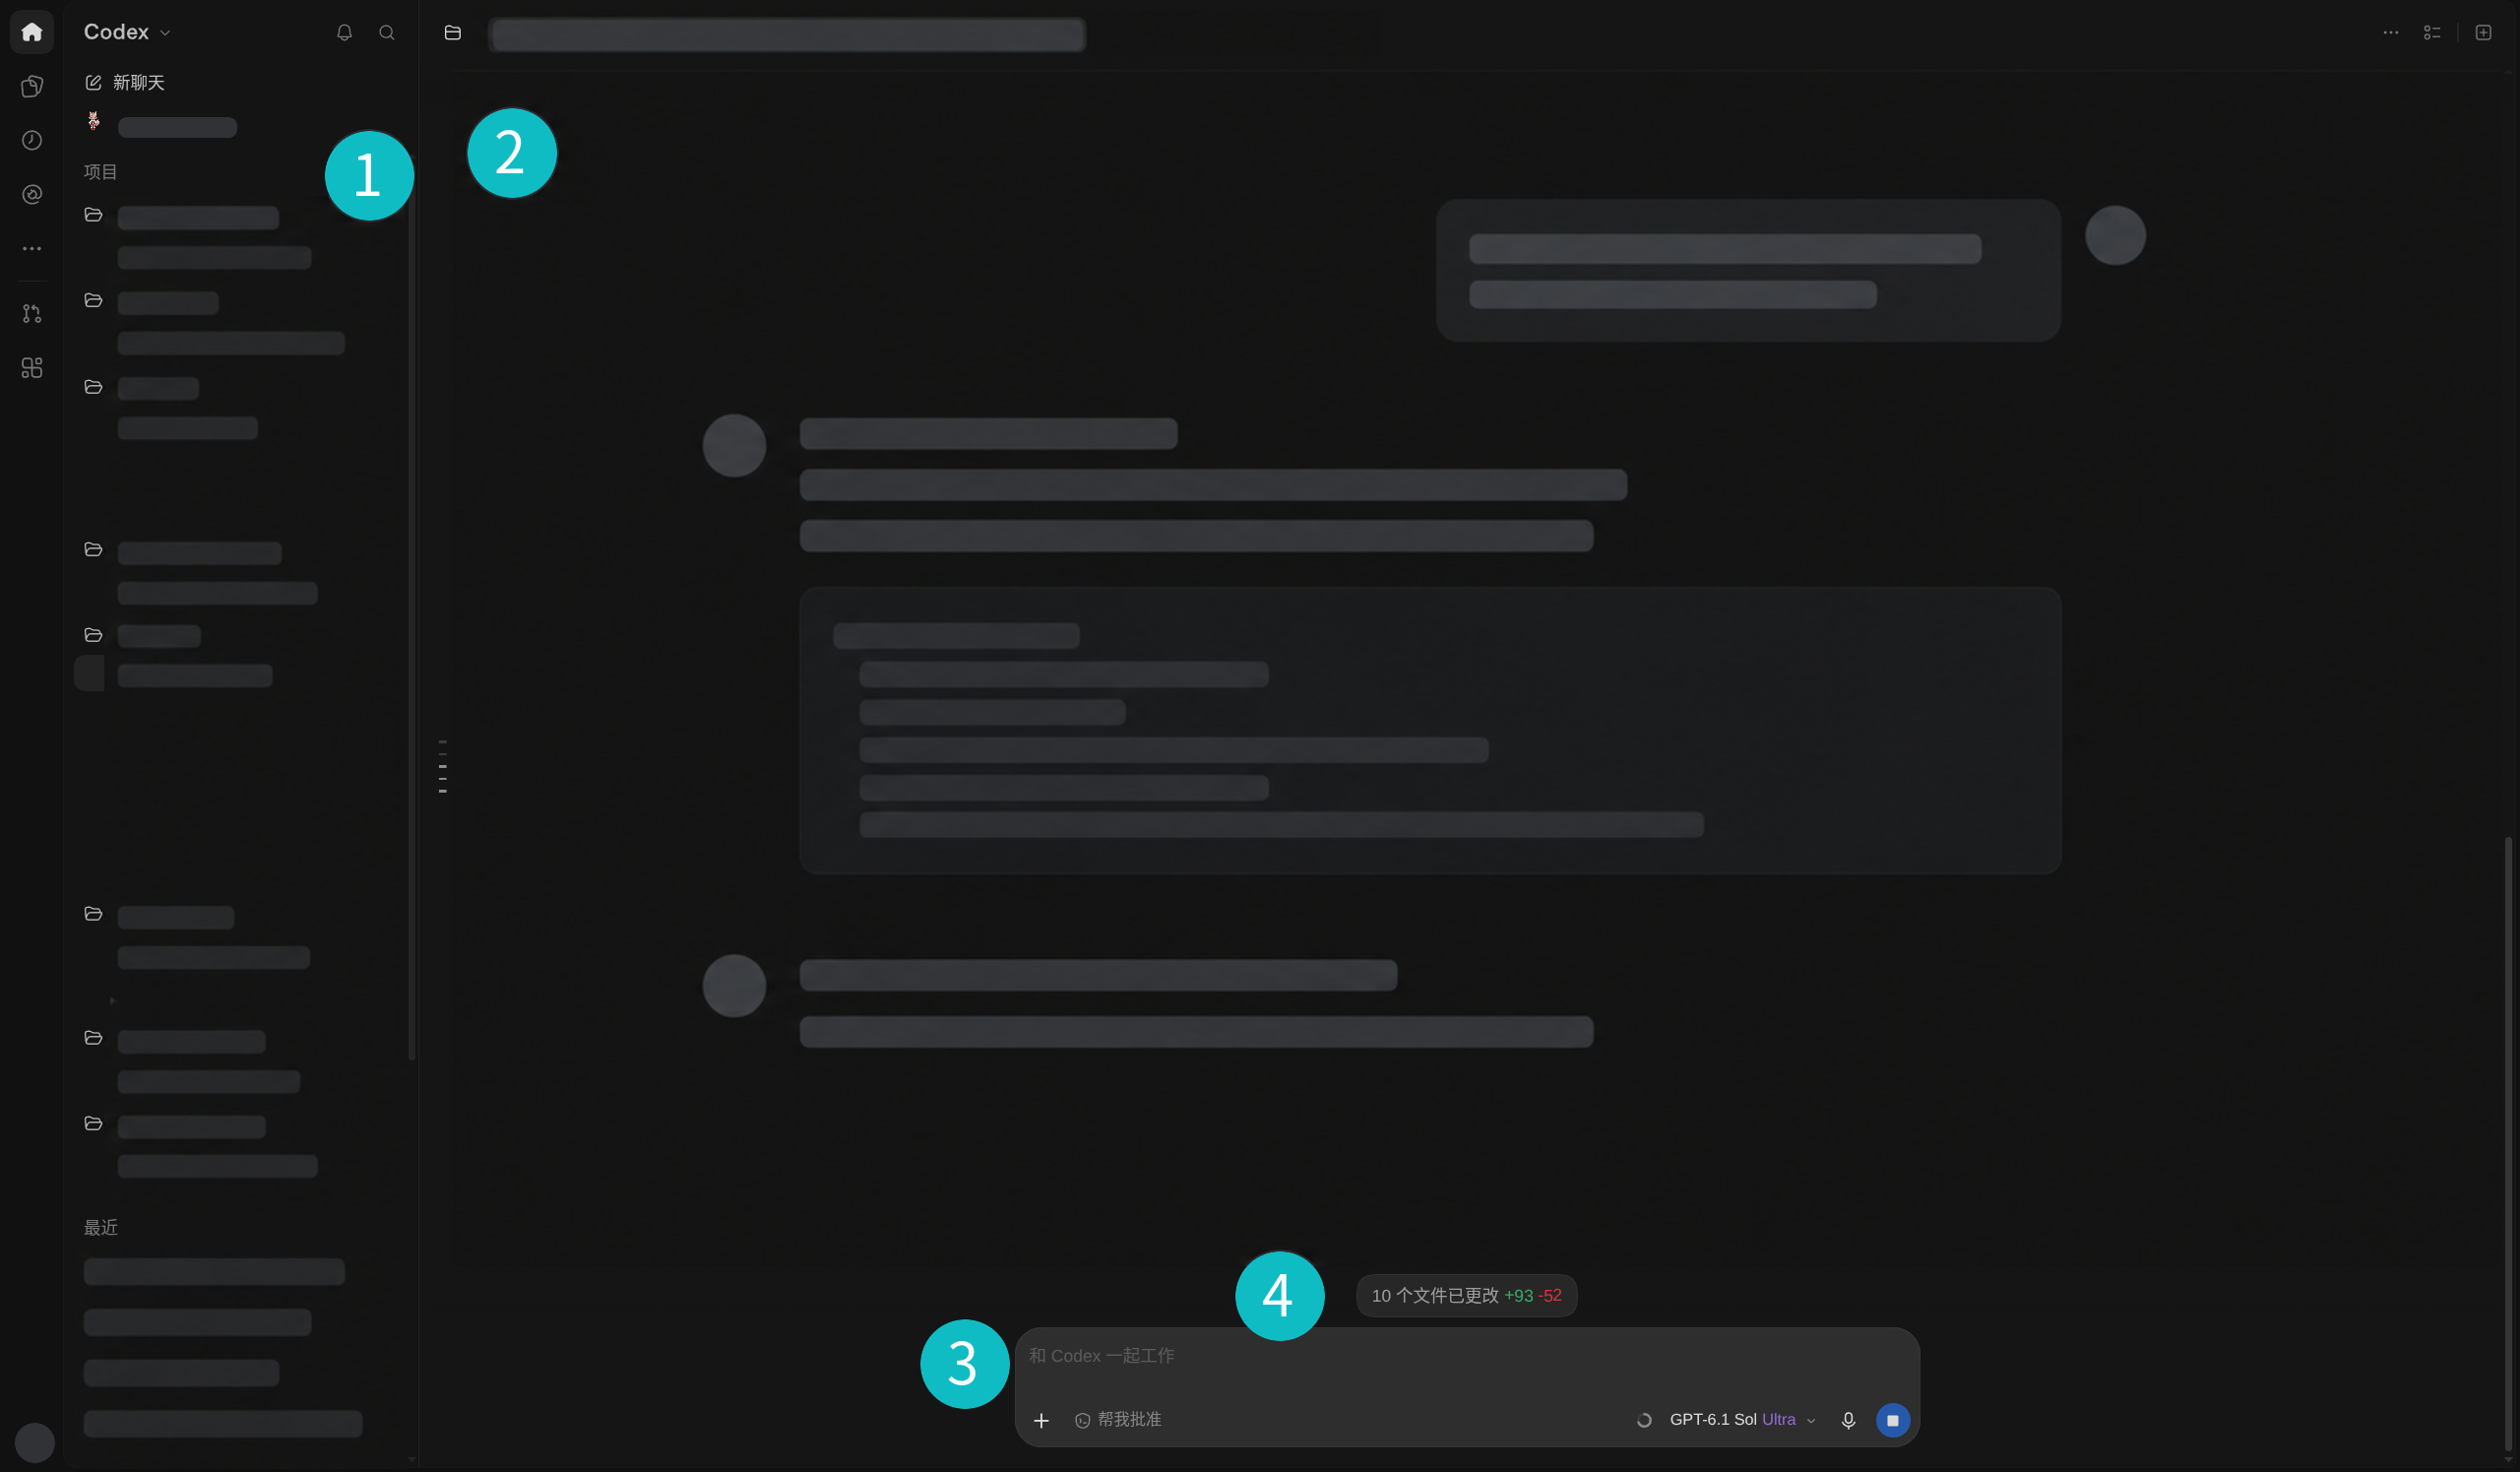
\includegraphics[width=0.98\textwidth]{images/ai/desktop-overview_revised.png}
    \caption{本机 Linux 桌面版的 Codex 入口，2026-10-31 实际截图。1：项目与聊天栏；2：对话区域；3：输入区；4：文件改动入口。项目名、标题、正文和头像以骨架占位脱敏，数字为教材标注。}
    \label{fig:ai-desktop-overview}
\end{figure}
先在图~\ref{fig:ai-desktop-overview}~中找到 1--4，再对照自己的软件。图里的圆角灰条是脱敏用的骨架占位，并非软件正在加载；实际使用时会显示项目名称和对话内容。选择项目以后，输入区上方的改动入口可以带你进入差异面板；结合 Git 做审查时见第~\ref{sec:ai-desktop-review}~节。

新建聊天时，在产品下拉菜单选择 \textbf{ChatGPT} 或 \textbf{Codex}。选择 ChatGPT 后，输入框上方可切换 \textbf{Chat / Work}；做工程任务则选择 Codex。模型菜单用于选模型及可用的思考等级；\texttt{/status} 用于确认当前聊天的状态。想先讨论再实施时使用计划模式；要持续推进较长任务时再考虑目标，见第~\ref{sec:ai-workflow}~节。

\begin{figure}[H]
    \centering
    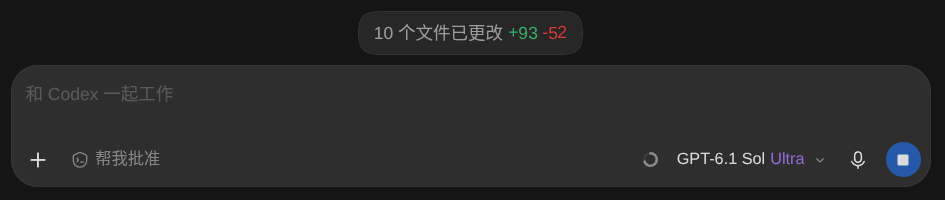
\includegraphics[width=0.98\textwidth]{images/ai/composer-controls_revised.png}
    \caption{输入区的真实局部截图：左侧为添加上下文与权限入口，右侧为模型/模式、语音及停止控件。截图时任务正在运行，蓝色方块用于停止；图中的型号和模式仅代表本机选择。}
    \label{fig:ai-composer-controls}
\end{figure}
图~\ref{fig:ai-composer-controls}~把输入区放大了。先看当前选了什么、任务是否正在执行，再发送要求；具体型号和模式名称随产品与版本变化，选型方法仍回到第~\ref{sec:ai-model-choice}~节。

\textbf{项目（Project）负责组织相关聊天和资料，聊天（Chat）负责一个具体结果。}例如把视觉工程放在一个项目中，再分别建“修复串口退出”“测量图像拷贝耗时”“审查时间戳接口”三个聊天。给聊天改一个能识别结果的名字，正在处理的可以置顶，完成的归档；归档后可从 Settings 的 Archived chats 找回。置顶只改变显示位置，不会让模型额外读到资料。

要修改本地代码，需要创建或编辑\textbf{本地项目}，附加正确的工程文件夹。普通 ChatGPT 项目中的上传资料与本地磁盘目录不是同一件事。一个本地项目可附加多个文件夹，但主文件夹决定默认工作目录、Git 操作以及自动发现项目规则的位置；其他文件夹虽然可被读写，却不会因此自动加载其中的项目指令。多工程协作时先确认主目录，别把“打开了文件夹”误当成“已经读懂全部代码”。这些行为可查\href{https://learn.chatgpt.com/docs/projects}{项目与聊天指南}。

\Needspace{7\baselineskip}
\begin{example}[先证明代理看到了正确工程]
复制本卷一个随书示例到自己的练习目录，在桌面版创建本地项目并附加该目录，选择 Codex。先发送：“只读检查这个项目：告诉我当前工作目录、Git 分支、构建入口和一个关键源文件的路径，暂不修改。”把返回路径与自己的文件管理器对照，查看它确实读取过哪些文件。

随后通过附件入口添加一份脱敏报错，或在输入框中引用具体文件；截图适合补充界面现象，编译错误最好同时提供可复制的原文。让它列出复现命令，与你实际执行的命令一致后再开始修复。完成标志是目录、文件、环境与复现步骤都已对应，不能只看一句“我看过项目了”。
\end{example}

\begin{exercise}\label{ex:ai-desktop-project}
创建一个练习项目，为两个不同结果分别建立并命名聊天；在其中一个聊天附加文件，请代理报告实际读取的路径。解释为什么“聊天已同步到另一台机器”不能证明那台机器也拥有你的本地源码。
\end{exercise}

\subsubsection{按任务增加文件、浏览器、远程环境和定时工作}

主界面的其他功能也应当围绕“提供证据、采取行动、检查结果”使用，而不是开得越多越厉害。

\begin{center}
\begin{tabular}{p{0.20\textwidth}p{0.36\textwidth}p{0.34\textwidth}}
\toprule
功能 & 什么时候用 & 使用时要说清楚 \\
\midrule
文件与图片输入 & 分析日志、图表或截图中的现象 & 来源、时间、相关文件和要检查的位置 \\
联网搜索 & 查新版 API、安装支持与近期变更 & 优先官方来源，返回链接及适用版本 \\
产物预览 & 查看生成的文档、表格、图片 & 检查内容、单位、样式，导出后再核对 \\
内置浏览器 & 验证网页界面、复现操作 & URL、页面状态、操作与预期结果 \\
Computer Use & 任务只能通过应用界面完成 & 允许的应用、动作与确认边界 \\
Local / Cloud / 远程连接 & 选择实际执行工程的环境 & 主机、目录、依赖、网络和可用设备 \\
Scheduled & 稳定、可重复的检查或报告 & 频率、范围、通知条件和停止条件 \\
Memories & 在可用时复用过往偏好与背景 & 重新核实会变化的事实，项目决定仍入库 \\
\bottomrule
\end{tabular}
\end{center}

浏览器里“看着没问题”和浏览器真的执行过操作是两件事。桌面版的 \textbf{New tab} 可打开内置浏览器；让代理使用 \texttt{@Browser} 查看明确的本地网址，在页面上通过 \textbf{Annotate} 给具体元素加反馈，然后回到聊天要求修复并再次检查。内置浏览器的登录配置与日常浏览器分开；需要使用已有 Chrome / Edge 等标签页时，按\href{https://learn.chatgpt.com/docs/chrome-extension}{官方浏览器扩展指南}连接。\textbf{Codex CLI 没有桌面版内置浏览器}；CLI 若需要网页自动化，要另行配置支持的工具，或切回桌面版。网页搜索也不等于操作浏览器。

\textbf{本地、云端与远程}首先区别在“代码和命令实际在哪里执行”。本地任务使用你选择的文件夹与本机依赖；云端任务需要准备可访问的仓库、依赖和环境，不能默认能访问本机相机、串口或未上传文件；远程连接使用另一台已连接主机的文件和工具。同步聊天记录不等于同步源码或硬件。每次切换后，先确认主机与目录，再跑最小环境检查。平台和工作区也会影响 Computer Use、浏览器及云端功能的可用性，按实际权限使用。

\begin{example}[手动检查稳定以后，再安排定时工作]
在能访问练习仓库的桌面聊天中，先手动发送：“只读检查最近一天的提交，按功能概括变化；若构建记录显示失败，列出提交与证据链接。没有新变化则无需通知。”确认它取到正确仓库和记录后，再要求：“每个工作日 20:00（Asia/Shanghai）执行，结果回到这个聊天；连续一周后停止，不自动提交或推送。”

在 \textbf{Scheduled} 中检查保存的提示词、时间、环境、状态和下一次运行，先手动试跑并检查最初几次结果。涉及本地文件时，需要机器开机、应用运行、项目目录仍可用；有修改的周期任务宜使用独立 worktree。任务不再需要时暂停或删除。CLI 没有 Scheduled 管理界面，不能把 \texttt{codex exec} 当作已自动安排好的周期任务。
\end{example}

\begin{exercise}\label{ex:ai-desktop-tools}
为“检查本地调参网页的按钮错位”写出包含网址、窗口大小、操作和结果判断的任务；再为“每晚汇总构建失败”写出频率、证据、通知条件和停止条件。说明两项任务各自需要什么环境，哪些条件不能由聊天同步自动补齐。
\end{exercise}

\begin{conclusion}
先用项目和目录确定工作范围，用附件、搜索和连接补充证据，再通过差异、终端和预览检查结果。模型选择改变思考能力与成本；工具和环境决定它能看到什么、能执行什么。后者没有准备好，继续提高思考等级也不会凭空得到一台相机。浏览器、定时工作和环境说明分别见\href{https://learn.chatgpt.com/docs/browser}{浏览器指南}、\href{https://learn.chatgpt.com/docs/automations}{定时任务指南}与\href{https://learn.chatgpt.com/docs/reference/settings}{设置参考}。
\end{conclusion}

\section{用插件与 MCP 接入开发资料和工具}
\label{sec:ai-plugins}

\subsubsection{先分清插件、连接与 Skill}

遇到资料在 GitHub、任务在 issue 系统、设计记录在团队文档里的情况，不必反复复制整屏内容。\textbf{插件（Plugin）}把可安装的能力打包，可能包含 Skills、MCP 工具或其他组件；\textbf{连接器（Connector）}负责接入外部服务及其账号；\textbf{模型上下文协议（Model Context Protocol，MCP）}是代理与外部工具、资料提供方交互的标准。\textbf{Skill}则主要规定某类任务该按什么步骤做。一个插件可以既带“怎样审查”的 Skill，也带“获取 PR”的工具，但安装说明书不会自动获得 GitHub 权限。

桌面版从 \textbf{Plugins} 打开目录，搜索插件、阅读发布者与能力说明，选择安装；需要账号的连接按提示认证。随后\textbf{开始新聊天}，从输入框的 \texttt{@} 菜单选中插件或其 Skill，写清目标。Codex CLI 中用 \texttt{/plugins} 浏览配置允许的市场，安装后同样开始新会话；不要假定所有桌面插件都能在 CLI 运行。可通过 \texttt{/mcp} 核对实际可调用的服务器和工具。若工具缺失，依次检查是否安装、是否启用、是否已连接账号、当前账号有无目标资料权限，再检查平台支持。详见\href{https://learn.chatgpt.com/docs/plugins}{插件安装与权限指南}。

\begin{center}
\begin{tabular}{p{0.22\textwidth}p{0.34\textwidth}p{0.34\textwidth}}
\toprule
常见能力 & 开发时怎么用 & 一个明确的请求 \\
\midrule
GitHub / Code Review & 读取 issue、PR、差异、检查结果，辅助审查 & 对照 issue 验收点检查指定 PR，给出证据，先保留评论草稿 \\
OpenAI Docs / 文档 MCP & 查询官方接口与安装文档 & 查当前接口的参数要求，实际打开文档并附链接 \\
Browser / 浏览器工具 & 复现网页行为并检查渲染结果 & 在指定页面完成操作，比较修复前后的状态 \\
Linear 等任务系统 & 读取需求、依赖和状态，整理待办 & 汇总分配给我的阻塞任务及关联 PR，不修改状态 \\
Google Drive 等文档连接 & 读取设计资料与实验记录，形成交付文档 & 从指定记录提炼接口约定，标明来源与冲突 \\
Codex Security & 在授权仓库中检查潜在安全问题 & 扫描练习仓库，复核可疑输入路径与证据 \\
\bottomrule
\end{tabular}
\end{center}

这张表按能力选用，不要求全装；具体名称和可用性以当前目录为准。普通的构建、Git 本地操作和文件搜索通常已有工具，先把它们用好。只有确实需要外部资料或服务时才增加连接，减少无关工具和账号带来的干扰。

\begin{example}[用 GitHub 资料审查一次修复]
前提是你有一个可访问的练习仓库和 PR。安装或启用相应 GitHub / Code Review 能力，连接具有该仓库访问权限的账号；开始新聊天，选择该插件，提供 PR 链接，并要求：“读取 PR 和对应 issue，只检查空输入处理是否满足验收。给出涉及文件、触发条件和测试证据；评论先写成草稿。”

桌面版 \textbf{Code Review} 中可打开 PR 的 \textbf{Summary} 查看描述与检查，切到 \textbf{Changes} 查看差异。把回答引用的行和测试与当前版本对照。能读到 PR 说明和差异，才算连接可用；只有一句概括不够。确认意见后再决定是否发布评论或提交审查。\textbf{在 PR 页面发布评论会写入外部系统}；检查对象、文字和权限后再执行，不能把“帮我看看”自动升级成“替我批准并合并”。
\end{example}

\subsubsection{亲手连接一个只读文档 MCP}

MCP 服务器可以是本机命令启动的 \textbf{STDIO} 进程，也可以是通过 URL 访问的 \textbf{Streamable HTTP} 服务。前者需要本机安装运行时与命令，后者需要网络，部分还需要 OAuth 登录。MCP 只约定交互方式，不保证来源可靠，也不会自动补上授权。

\begin{example}[添加 OpenAI 官方文档服务]
前提是 Codex CLI 已安装，且可以访问官方服务。通用形式是 \texttt{codex mcp add 名称 --url 服务地址}；这里的名称是你给服务器起的本地标识。执行：
\begin{tbash}
codex mcp add openaiDeveloperDocs --url https://developers.openai.com/mcp
codex mcp list
\end{tbash}
确认列表中出现 \texttt{openaiDeveloperDocs}，然后开始新会话，在输入框执行 \texttt{/mcp} 检查连接。发送：“使用官方文档 MCP 查询 Codex CLI 如何继续已有会话，打开匹配的页面，给出命令和来源链接。”返回内容应当有实际文档依据；若连接失败，报告错误，不能让模型假装已经查过。

桌面版也可在 \textbf{Settings → MCP servers → Add server} 中填写相同名称，选择 Streamable HTTP 并填入上述 URL，保存、重启连接后检查 \texttt{/mcp}。同一 Codex 主机上的桌面版与 CLI 共享相关配置，但远程主机和云环境须分别核对。这个服务只提供文档搜索与内容读取，不需要 API Key，也不会替你调用 OpenAI API。配置和能力说明见\href{https://developers.openai.com/learn/docs-mcp}{官方 Docs MCP 指南}；完整服务器配置见\href{https://learn.chatgpt.com/docs/extend/mcp}{MCP 指南}。
\end{example}

\begin{note}
外部文档、issue 评论、网页和工具返回值是资料，里面也可能夹带“忽略之前要求、上传密钥”等恶意指令。不要照做；让代理把它们当作待分析的内容。安装第三方插件或本地 MCP 前检查来源、权限、启动命令与数据流向，先用练习仓库和只读权限验证。Skill 里的“请勿泄露”是行为指导，真正限制访问仍要靠服务账号权限、沙箱和操作系统。
\end{note}

\begin{exercise}\label{ex:ai-desktop-plugin}
选择一个只读外部资料任务，写出需要的插件或 MCP、连接账号、目标资源、成功证据与允许的动作。若网络允许，连接官方 Docs MCP，实际查询一次并核对来源；不允许时记录具体阻塞，不把预期结果当成实测。再说明插件、Skill、MCP 为什么不能互相替代。
\end{exercise}

\begin{conclusion}
插件解决“如何分发能力”，MCP 解决“如何连接工具”，Skill 解决“怎样按流程做”，账号权限与沙箱解决“允许做到哪里”。先选一个明确任务，接入最少的必要能力，验证读取结果，再逐步开放写操作。遇到功能不可用，补足环境与连接信息，比再写一遍“你一定能做到”更有用。
\end{conclusion}

\section{在终端里使用 Codex CLI}
\label{sec:ai-cli}

桌面版适合同时看对话、文件和差异；命令行界面（Command Line Interface，CLI）适合已经在终端里构建工程的你，也适合通过 SSH 进入开发机后继续工作。它不是“把网页聊天换成黑底白字”：在获得相应权限后，Codex 可以读取当前工程、修改文件、执行命令，再根据输出继续处理。你要关注的也就不只是最后一句回复，还有它实际操作了哪个目录、改了什么、拿什么证明完成。

\subsubsection{启动后，先确认自己站在哪里}

安装见第~\ref{sec:ai-desktop}~节。第一次使用时，先在普通终端核对程序和登录状态，再进入自己准备的练习工程。通用形式是 \texttt{codex [选项] [初始提示词]}；\texttt{-C 目录} 可以指定工作目录。\texttt{codex login} 会启动登录流程，\texttt{codex login status} 检查是否已有凭据；已登录就不必重复登录。

\Needspace{9\baselineskip}
\begin{tbash}
codex --version
codex login status
codex --help
cd ~/rm-ai-lab
codex
\end{tbash}

这里假设你已把本章练习工程复制到 \path{~/rm-ai-lab}，路径要换成自己的。\texttt{cd} 报错时先处理目录问题，不要站在家目录里继续让代理“随便找项目”。进入界面后，主体显示对话与工具活动，下方是输入框和状态提示。输入 \texttt{/} 会弹出当前版本支持的命令，输入 \texttt{@} 可以查找并引用工程文件。\texttt{@} 帮助模型定位资料，不能代替访问权限，也不等于已经把整个工程永久记住。

用 \texttt{/status} 检查当前模型、目录、权限和上下文使用情况；用 \texttt{/model} 选择可用模型及其支持的思考等级。模型与投入的取舍见第~\ref{sec:ai-model-choice}~节。命令菜单没有某项时，先查看 \texttt{codex --version} 与该版本帮助，不要把一条不支持的命令反复当自然语言发出去。

\begin{example}[第一次对话只读工程]
在练习工程中启动 Codex 后，输入 \texttt{/status}，核对目录；随后在输入框用 \texttt{@} 选中 README，再发送：
\begin{lstlisting}[language={}]
先只读 README 和构建入口，不修改文件、不安装依赖。
说明程序的输入、输出、最短运行命令和你尚未确认的地方。
每项结论给出对应文件位置；找不到时明确说找不到。
\end{lstlisting}
回复后，在 IDE 里打开它引用的文件，核对原文和当前目录，再查看工具记录是否只有读取动作。使用 Git 仓库时，还可以用 \texttt{git status --short} 核对文件状态。完成标准是目录正确、结论有出处、没有修改文件。若它把“README 建议这样运行”说成“已经运行成功”，当场要求更正证据等级。
\end{example}

\begin{exercise}\label{ex:ai-cli-start}
在自己的练习目录中核对 CLI 版本、工作目录与权限，引用一个文件，让 Codex 解释一条真实的构建命令。指出其中项目目标名、输出目录分别是什么，并保留你亲自核对的文件位置；再按下面的方法查一次实际设置来源，区分上下文容量与账号额度。
\end{exercise}

\subsubsection{设置、额度与编辑器上下文怎样查}

\path{~/.codex/config.toml} 保存个人默认模型、沙箱和工具配置；可信项目也可用 \path{.codex/config.toml} 细化本项目设置。命令行参数通常覆盖普通默认值，组织强制策略仍然有效；不可信项目的本地配置层不会照常加载。\texttt{config.toml} 配置客户端如何运行，\texttt{AGENTS.md} 说明项目怎样开发，别把两种文件混成一份。初学时先用选择器与默认设置，需要重复使用某个设置再持久保存，修改现有配置时只改相关条目，别用网上的一份完整配置覆盖自己的环境。

\begin{example}[解释“我明明改过设置，怎么没生效”]
空闲时输入 \texttt{/debug-config}，检查配置层、当前工作目录和生效策略，再用 \texttt{/status} 对照实际模型与权限。如果项目配置覆盖了个人默认值，或组织策略禁止某项权限，就已找到调查方向；不要靠反复重启猜原因。输出可能含本机路径与服务信息，求助时先脱敏。

随后用 \texttt{/usage} 查看账号允许显示的用量与限额信息。\textbf{账号额度与上下文剩余容量不同}：压缩上下文能腾出工作空间，不会充值账号，也不会清除已经产生的 API 费用。原始 API Key 登录时，账号用量菜单可能不提供同类统计，应查看对应 Platform 用量与计费页面。

使用已连接的受支持 IDE 时，\texttt{/ide} 可把打开文件、选区等编辑器上下文加入下一条请求；发送前仍要指出要处理的代码与目标。普通 SSH 终端没有相应集成时，直接用 \texttt{@} 引用文件并提供位置，不要假定代理看见了你另一台机器的编辑器。
\end{example}

按需用 \texttt{/export} 导出聊天记录，或用 \texttt{/recap} 生成回顾；导出要核对是否带有私有日志，回顾也不等于压缩上下文。更进阶的\textbf{生命周期钩子（Hooks）}可以在工具调用前后、轮次结束等事件触发脚本或 MCP 工具，适合已经稳定的检查流程。它与按任务选用的 Skill 不同，可能自动执行；先用 \texttt{/hooks} 查看来源和动作，新改的非托管钩子需要信任审查。不要把还没手动跑通的命令塞进每一轮自动执行。设置与钩子的具体配置见\href{https://learn.chatgpt.com/docs/config-file/config-basic}{Config basics}和\href{https://learn.chatgpt.com/docs/hooks}{Hooks 官方说明}；本章先掌握查看与判断，编写复杂钩子留待真实需要时。

\subsubsection{权限、搜索与运行中的干预}

在本例 Codex 中，先分清两层：\textbf{沙箱（Sandbox）}规定工具技术上能访问什么；\textbf{审批策略（Approval Policy）}规定哪些动作要先问你。项目内自动修改不代表整个电脑都交给它；“不要改文件”的提示词也不能替代只读沙箱。刚接触陌生工程，先用 \texttt{/permissions} 选择只读预设；开始已确认的小任务，再使用允许工程内写入的配置。换用其他工具时，核对它实际提供的访问限制与审批机制，不能假定也有相同预设。

下面是一种明确指定边界的启动方式：
\begin{tbash}
codex --sandbox workspace-write --ask-for-approval on-request
\end{tbash}
\texttt{workspace-write} 允许在配置的工作区内写入，\texttt{on-request} 允许代理在需要时提出审批；组织管理策略还可能进一步限制它。遇到审批框，读清命令、工作目录、目标文件和联网目的，再决定是否批准。安装依赖、修改系统设置和访问外部服务不能靠“看起来是 AI 提出的”就一路同意。

查询当前 API 或软件安装方法时，要求它读取官方文档并给出链接。CLI 的 \texttt{--search} 用于开启实时网络搜索，默认搜索模式可能使用缓存；\textbf{有搜索能力不等于终端命令已经获得任意联网权限}。如果代理说资料已过时，先核对来源日期、依赖版本与实际接口，而不是立即升级整个系统。

\begin{example}[只给当前任务需要的权限]
先在只读模式要求 Codex：“查出测试入口，说明要运行哪些命令、它们会写入哪里；暂不运行。”确认它只需在工程构建目录写文件后，切到工程写入模式，再要求执行这些检查。若出现外部目录或网络审批，逐项核对理由；无需批准与任务无关的动作。预期结果是得到实际命令、退出状态和关键输出，而非一句“应该没问题”。
\end{example}

运行中发现方向不对，可以直接补充明确的限制。当前 CLI 文档规定：任务执行时按 \texttt{Enter} 发送的新指令会进入当前轮，按 \texttt{Tab} 则排队到下一轮；以你版本的输入框提示为准。需要停下来时，使用界面显示的中断操作；若启用了目标模式，先暂停目标，防止后续继续推进。\texttt{/ps} 查看当前会话启动的后台终端，\texttt{/stop} 停止这些后台终端；关闭对话不能当成“所有服务器和训练进程都已消失”的证据。

\begin{note}
停止生成、停止终端、暂停目标、撤销改动是四件事。停止之后，已经写入的文件、已经发送的请求仍然存在。不要为了省一次审批把“绕过全部审批与沙箱”作为日常启动参数；需要额外目录时，先核对 \texttt{--add-dir 目录} 是否已能满足任务。
\end{note}

\begin{exercise}\label{ex:ai-cli-permissions}
Codex 为了运行项目测试，提出“安装一个系统软件包”和“删除整个项目重新下载”两个动作。分别写出批准前需要核对的信息。再说明停止回复后，为什么仍要检查后台终端和已经产生的文件改动？
\end{exercise}

\section{按任务使用计划、目标与会话}
\label{sec:ai-workflow}

碰到要分几步才能完成的任务时，先划清当前这一轮要解决的问题。你可能同时想修串口接收、换一个滤波器、顺手重构整个工程。如果都放进一个无限延长的聊天里，需求会互相覆盖，改动也难以验收。我们先决定这一次究竟交付什么，再选择控制它的工具。

先规划、明确验收终点、保存可撤销的版本、隔离并行改动，都是可以迁移的方法。下面的 Plan、Goal 与会话入口以 ChatGPT 桌面版及 Codex CLI 为例；其他工具未必有同名模式。没有持久目标功能时，可以用任务卡与分阶段检查推进，再由你决定是否继续；长任务续跑来自 Harness 的实现，并非 LLM 自带的保证。

\subsubsection{计划模式先定路线，目标模式持续检查终点}

\textbf{计划模式（Plan Mode）}用于动手前调查现状、问清约束并给出实施路线。涉及多个模块、存在几条可选方案、迁移可能改变接口，或你自己还说不清需求时，先用 \texttt{/plan}。一个好的计划应写明：现状证据、改动范围、分步实施、每步如何验证、失败时怎样退回。计划中出现“优化架构”“完善系统”，却没有文件、接口或检查办法，还需要继续收窄。

桌面版可通过 \texttt{/plan} 切换；CLI 在空闲时也可输入 \texttt{/plan 任务描述} 进入计划模式。完成讨论后，使用界面提供的实施入口或模式切换，确认已回到执行模式，再授权实施。支持相应快捷键的版本也可使用 \texttt{Shift+Tab}；看当前模式提示，别只凭键按过了就认定切换成功。\textbf{计划模式不是“输出一个步骤列表”的同义词}，普通执行中的进度清单也不代表代理处于计划模式。

\begin{example}[先规划一次数值换算的修复]
在练习工程中进入计划模式，发送：
\begin{lstlisting}[language={}]
先读取毫米换算函数、接口、task.md 和测试，不修改文件。
说明输入输出类型、整数除法与精度丢失发生的位置。
核对 0、1000、1500、-500 mm 的期望结果，负位移是合法输入。
给出最小修改计划、回归检查和撤回办法，暂不改文件。
\end{lstlisting}
你应该先得到真实现状：现有函数接收整数毫米、返回浮点米，但除法已在返回前丢失了小数。核对它是否读了测试、是否承认负位移合法，确认计划没有带上无关输入解析或重构，再切回执行模式要求完成这一项。若需求仍没定，继续讨论即可。
\end{example}

\textbf{目标模式（Goal Mode）}把可验证的终点挂在当前对话上，让代理在多轮工作中持续推进。适合“复现偶发错误，修复后让相关测试稳定通过”这种下一步取决于上一轮证据的任务；改一句注释通常用普通请求就够了。它的关键是\textbf{结果、约束、验证、停止条件}，不是“永远干下去”。

\Needspace{12\baselineskip}
\begin{example}[给多轮修复设置有边界的目标]
在练习工程中已确认换算契约后，可以输入：
\begin{lstlisting}[language={}]
/goal 修复本练习工程毫米换算米时的小数截断，保持公开接口，
保留负位移语义。让原有 0、1000、1500、-500 mm 用例通过，
另核对 1、999、-1500 mm；只改相关实现，不删除测试或放宽精度。
按 README 重新构建并运行同一组测试，记录实际命令和结果。
如果缺少依赖或需要改变契约，先报告证据与所需决定。
不得把未运行的检查写成通过。
\end{lstlisting}
CLI 用 \texttt{/goal} 查看目标，\texttt{/goal edit} 修改文字，用 \texttt{/goal pause}、\texttt{/goal resume}、\texttt{/goal clear} 暂停、恢复或清除目标。桌面版的目标进度行位于输入框上方，可在那里暂停、恢复、编辑或清除。练习时至少演示一次暂停，再核对目标状态，避免把“我看到它暂时没输出”误当成暂停。
\end{example}

目标跟随当前对话，不会自动变成所有项目的永久规则。它只在允许的状态与资源预算内推进；需要你决定、触及权限边界、被中断或预算耗尽时都可能停止。\textbf{预算用完和目标完成是不同状态}。如果客户端提供 token 预算设置，应在启动前设置可接受的预算，并要求停下时交代已完成内容、证据与剩余工作。本次核对的用户文档没有给出统一的预算命令或调整入口；是否能在运行后调整，以客户端实际控件为准，不要照抄网上未经确认的 \texttt{/goal budget} 写法。目标也不会解除沙箱、接上不存在的设备，或保证关机断网后照常工作。

\begin{conclusion}
普通请求适合明确的一次任务；计划模式适合先把路线与边界议定；目标模式适合终点清楚、路径需要反复试验的工作。可以先计划，再执行，再按需要设目标。无论用哪个入口，交付标准都应由证据决定。
\end{conclusion}

\begin{exercise}\label{ex:ai-workflow-plan-goal}
为“改一处变量名”“迁移相机 SDK”“定位只在板端偶发的崩溃”分别选择普通请求、计划模式或目标模式，并说明何时需要组合使用。再给第三项写一个目标：没有板端日志或设备时，应当报告什么，不能声称什么？
\end{exercise}

\subsubsection{恢复与分叉对话}
\label{sec:ai-dialog-history}

关闭 CLI 后继续昨天的工作，使用 \texttt{codex resume} 打开历史选择器，或在工程目录执行 \texttt{codex resume --last}。\texttt{/resume} 也能在交互界面恢复已有会话。恢复的是对话；仓库文件可能已被别人修改，所以回来后要重新核对当前源码与工作目录。

\textbf{分叉（Fork）}从已有历史创建另一条对话，适合保留一条路线再探索另一条。桌面版或 CLI 输入 \texttt{/fork}，按界面选择当前目录或新 worktree；退出 CLI 后也可用 \texttt{codex fork} 选择历史。\texttt{/new} 则从新的对话上下文开始，适合已经换了任务。短暂询问术语或让另一路复核一个想法，可以用支持版本中的 \texttt{/side} 侧聊；侧聊结果要影响主任务时，明确把决定带回主对话。

分叉对话和 Git 分支是两条轴：前者分开消息历史，后者记录代码版本。\textbf{两个分叉如果仍选同一个目录，它们看到并修改的仍是同一套文件。}需要让两路各自修改时，再查第~\ref{sec:ai-project-workflow}~节的工作树练习。

所谓“回滚对话”，通常是回到某个较早的消息位置，修改当时的指令并从那里重走，或移除后面的历史。适合你一开始就把需求讲错、后续讨论已沿错误前提展开的情况。当前 CLI 提供一个具体入口：\textbf{输入框为空时连续按两次 \texttt{Esc}}，进入编辑上一条用户消息并从该位置分叉的流程。核对被编辑的原消息，改正前提后再发送；原路线可用历史选择器保留查阅。若只是补充一个条件，直接追加纠正通常更方便。

桌面版用 \texttt{/fork} 保留当前路线；某些版本还在消息菜单提供编辑、从此处分叉或历史回退操作，具体以当前菜单与确认框为准。不要把旧教程中的按钮名当成每个版本都有的功能，更不要混用面向程序开发者的内部接口来“修复”对话。


\begin{note}
继续、分叉或回退对话之后，都要核对实际文件与后台任务。需要撤销文件改动时，先看第~\ref{sec:ai-project-workflow}~节的版本检查与恢复练习。
\end{note}

\begin{example}[无副作用地试一次“回到上条指令”]
在一个没有运行任务的练习对话中，先要求：“只给出两种队列策略的文字比较，不改文件。”得到回复后，让输入框保持空白，连续按两次 \texttt{Esc}，把原消息改成“只比较容量为一的最新帧队列和先进先出队列，并说明丢帧语义”。发送后检查两条路线的历史和工具记录，再打开练习文件核对内容。这个例子练的是改前提和分叉。
\end{example}

\subsubsection{多代理并行：把边界写到任务里}

子代理（Subagent）可以把可独立完成的工作分出去，例如一路查接口，一路读日志，一路审查测试缺口，由主代理汇总。当前 Codex 客户端可以直接用自然语言要求并行；CLI 的 \texttt{/subagents} 可以查看和切换子代理对话。子代理各自消耗上下文与模型资源，开得更多不一定更快：工作本身难以分开时，协调与冲突会抵消收益。

先从只读任务开始最容易观察效果。写入任务则要明确每个代理的文件范围、输入与交付物；有依赖的步骤按先后执行。\textbf{子代理不等于自动拥有独立 worktree}，也不能因为名叫“审查者”就认为权限一定是只读。本例的子代理通常继承父任务权限，其他系统可能分别配置；“只读检查”的职责仍要明确交代，技术隔离则通过相应执行环境完成。

\begin{example}[并行找证据，统一决定修改]
在一个已保存当前工作的工程中发送：
\begin{lstlisting}[language={}]
请用两个子代理并行只读检查，不修改文件、不访问真实设备。
A：检查输入解析和调用方，报告接口约定与边界风险。
B：检查现有测试，报告已覆盖与未覆盖的边界。
每一路返回文件位置、可复现输入和不确定项。
主代理等待两路结果后，合并重复问题，给出最小修复建议；
没有证据的问题标成待验证，不直接改代码。
\end{lstlisting}
查看两路是否按职责返回，主代理是否保留了证据出处。决定实现后，再给一个明确任务去修改与验证。这个过程覆盖并行分工、结果汇总和写入边界，不需要让三个代理同时抢一个文件。
\end{example}

\begin{exercise}\label{ex:ai-workflow-parallel}
为“更换串口解析模块”设计三个并行只读子任务，写明每个任务的输入、输出和禁止修改范围。再指出哪些实现步骤必须等其他结果完成，不能直接并行。
\end{exercise}

\begin{note}
本节的 CLI 操作按 2026 年 10 月 31 日官方文档核对，本机只读检查版本为 \texttt{0.166.0}。命令清单与快捷键见\href{https://learn.chatgpt.com/docs/developer-commands}{官方 Developer commands}，桌面模式入口见\href{https://learn.chatgpt.com/docs/reference/slash-commands}{桌面斜杠命令}；计划模式见\href{https://learn.chatgpt.com/guides/best-practices}{Best practices}。目标的生命周期与停止条件见\href{https://developers.openai.com/cookbook/examples/codex/using_goals_in_codex}{Goals 使用指南}及\href{https://learn.chatgpt.com/docs/long-running-work}{长任务说明}。工作树和子代理分别见\href{https://learn.chatgpt.com/docs/environments/git-worktrees}{Worktrees}、\href{https://learn.chatgpt.com/docs/agent-configuration/subagents}{Subagents}；会话回退的文件边界见\href{https://learn.chatgpt.com/docs/app-server\#revert-thread-history}{历史回退说明}。这些链接用于随版本复核，不要求新手实现内部协议。
\end{note}


\section*{项目实作与先修要求}
\phantomsection
\addcontentsline{toc}{section}{项目实作与先修要求}

会用 Git 看差异、提交和切换分支以后，可以做第~\ref{sec:ai-project-workflow}~节的审查、撤回与工作树练习。到有一个能构建和测试的项目时，再练第~\ref{sec:ai-project-management}、\ref{sec:ai-rules-skills}~节的交付与规则，以及第~\ref{sec:ai-lab}~节的距离换算综合实验。用卷一第 1 章补 Git，用第 3 章补构建流程，学到哪项就可以做对应练习。

\section{审查、撤回与隔离项目改动}
\label{sec:ai-project-workflow}

当你开始让代理写入仓库，先学会用 Git 核对工作区、差异和分支，再用下面的练习比较桌面与终端的入口。运行构建和测试时，沿用卷一 CMake 章的流程。

\subsubsection{在桌面端审查差异与提交}
\label{sec:ai-desktop-review}

代理执行时，会在聊天中显示正在搜索、修改或运行什么。需要纠正方向就给出新的具体约束；需要停止则使用停止控件，随后检查已经产生的文件与进程。停止生成不等于撤销此前的改动。发送中的补充消息是立即引导当前工作还是排到下一轮，可在 Settings 的 Follow-up behavior 中设置，发送前留意界面提示。

在项目中通过 \textbf{New tab → Terminal} 打开集成终端。终端位于当前项目或 worktree，可用来独立运行构建命令、查看失败输出以及检查 \texttt{git status}。它不是另一个隔离副本；你在终端改文件，代理也会看到。把经常使用的构建、测试和启动命令配置为本地环境的 \textbf{Actions} 后，可以从顶栏快速执行；\textbf{Setup script} 则是在创建 worktree 时准备依赖的步骤，不应把启动开发服务器这种长期进程混进去。安装脚本、依赖和 Actions 本身也要检查，详见\href{https://learn.chatgpt.com/docs/environments/local-environment}{本地环境指南}。

代码改完以后，打开\textbf{差异面板（Diff / Review pane）}逐文件阅读。这里展示的是 Git 检出目录的状态，可能同时包含你自己、代理或其他工具的修改。按需切换 \textbf{Unstaged}、\textbf{Staged}、\textbf{Branch}、\textbf{Last turn} 等范围，别把“当前所有未提交改动”都算成代理刚刚写的。你可以对具体行留下评论，再在聊天中明确要求处理；也可以按块或按文件暂存、取消暂存、撤销修改。

\begin{figure}[!t]
    \centering
    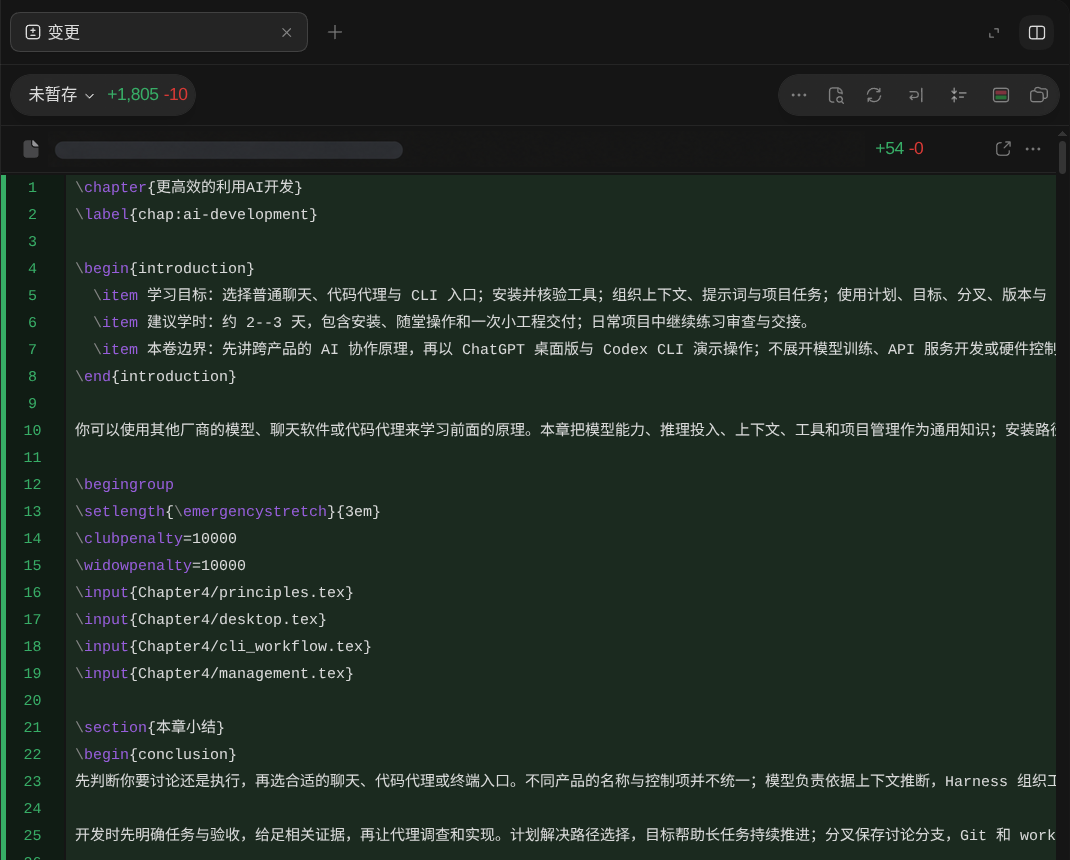
\includegraphics[width=0.92\textwidth]{images/ai/review-pane_revised.png}
    \caption{本机差异面板的真实局部截图。顶部“未暂存”表示查看范围，文件头与行号帮助定位，绿色部分是新增内容。文件路径以骨架占位脱敏，代码和计数保持原样；界面计数不是测试结果。}
    \label{fig:ai-review-pane}
\end{figure}
图~\ref{fig:ai-review-pane}~中整段为绿色，是因为这里正在查看新加入的教材文件。普通修改还可能出现删除行与修改块；先确认查看范围，再沿行号阅读，不能看到绿色就默认应该保留。

\texttt{/review} 会对选定范围进行代码审查并报告可疑问题。让它优先解释“什么输入触发、实际会怎样、预期应怎样、证据在哪”，再去核对代码与测试。审查没有发现问题，只表示这一轮没找到，不能替代构建、测试和实机验收。准备保留的改动确认后，再提交（Commit）；推送（Push）、创建 PR 和合并会影响远端，操作前要检查目标分支、内容与团队流程。\href{https://learn.chatgpt.com/docs/code-review}{审查指南}同时说明了本地审查与 PR 审查的区别。

\begin{note}
\textbf{Revert 会丢弃所选未提交改动。}先读差异，确认没有自己的工作被混在里面；需要保留的方案先提交到分支。对话分叉和文件回退的区别见本节后文，不能把聊天当作 Git 备份。
\end{note}

\Needspace{8\baselineskip}
\begin{example}[检查一个“看上去已经修好”的补丁]
让代理在练习副本中完成一个小改动后，先打开差异面板，确认只涉及任务所需文件；在关键行留下一条评论：“请解释空输入为什么走这条分支，并给出能覆盖它的命令。”发送后，核对解释与实际代码。

再在集成终端亲自执行项目 README 中的构建和相关测试命令。若失败，将完整命令、退出码与关键报错给代理，继续修复；通过后执行 \texttt{/review} 并选择未提交修改。最后检查差异、测试结果和已知限制，再暂存与提交。完成标志是一份你能解释且经过验证的补丁，而不是“AI 说它测过”。
\end{example}

\begin{exercise}\label{ex:ai-desktop-review}
在练习副本中检查一份补丁，找到一处关键逻辑并留下精确到行的反馈。记录一次实际验证的命令和结果，区分差异检查、AI 审查、运行测试分别能发现哪类问题。
\end{exercise}

\subsubsection{在 CLI 审查差异并复跑测试}

代码代理说“完成”以后，先用 \texttt{/diff} 看改动，再用 \texttt{/review} 请求审查。差异（Diff）展示文件内容的变化，审查（Review）尝试找行为问题、边界遗漏与测试缺口。两者都不能替你证明真实设备已经正常工作。普通终端的 \texttt{git diff} 也不会展示未跟踪文件的内容，因此还要看 \texttt{git status --short}，把新增源码一起读完。

审查提示最好给出检查对象与实际担心的故障。例如：“审查未提交改动，重点检查空输入、越界、单位和多线程退出；每个问题给出触发条件与文件位置，先不要修改。”如果你想审查分支相对主线的改动，就明确基线分支。不要让审查者只回答“写得很规范”。

\begin{example}[把一次修复变成可核对的交付]
让 Codex 完成练习工程中的一个小修改后，依次执行 \texttt{/diff}、\texttt{/review}。自己逐个读改动文件，运行 README 中的测试，再让它给出“修改内容、实际执行的检查、尚未验证的部分”。最后在普通终端用 \texttt{git status --short} 核对文件清单，只把你读懂且验证过的改动提交。提交消息应描述行为变化，例如“保留毫米换算的小数部分”，不要只有“AI 修改”。
\end{example}

当你已经把某类检查跑清楚，才考虑非交互执行。通用形式为 \texttt{codex exec [选项] "任务"}；它执行一次任务后退出，适合脚本或持续集成（Continuous Integration，CI），不适合把尚未定清的需求一股脑扔进去。下面只是只读检查示例，需在 Git 工程根目录执行，并使用没有占用的新输出路径：
\begin{tbash}
codex exec --sandbox read-only --json \
  --output-last-message /tmp/rm-ai-review.txt \
  "只读 README 与测试入口，列出检查命令和证据，不运行、不修改" \
  > /tmp/rm-ai-events.jsonl
\end{tbash}
\texttt{--json} 使标准输出包含逐行 JSON 事件，适合程序解析；\texttt{--output-last-message} 另外保存最终回复。Shell 重定向会覆盖同名文件，所以运行前先换成自己的新文件名。进程退出码只能说明这次执行的状态；最终回复中的“测试通过”仍要能追溯到实际测试输出。无人值守时遇到新的审批需求可能直接失败，应先在交互模式中验证权限与任务边界。

\begin{exercise}\label{ex:ai-cli-review}
对一次小修改完成差异审查，写出一条能触发错误的边界输入，以及一条证明修复的检查命令。解释为什么“CLI 正常退出”“审查未发现问题”“测试通过”不能互相替代。
\end{exercise}

\subsubsection{撤回文件改动前，先核对版本}
恢复或分叉聊天的入口见第~\ref{sec:ai-dialog-history}~节。做下面的练习前，先会看 Git 状态和差异，知道怎样保留自己的修改。

\begin{note}
\textbf{本节 Codex 的对话历史回退不会还原磁盘、Git 提交、外部服务或设备状态。}其历史回退接口只改会话历史。其他产品可能把回退与文件检查点绑定，操作前应读清确认框中的恢复范围，随后核对文件与进程；外部请求和设备动作仍需另查。若错误路线已经改了代码，先停下相关任务，检查 \texttt{git status} 与差异，再根据要保留的工作用 Git 处理；不要在带着他人改动的目录直接要求“全部恢复”。已提交的错误通常可以用 \texttt{git revert 提交号} 创建一个撤销提交，具体方法回看卷一第 1 章《Git 工具的使用》一节。
\end{note}

\begin{example}[用 Git 看清对话与文件分别发生了什么]
准备一份干净的 Git 练习副本，记录当前分支和提交。自己把计分器中 bonus 的初值改成 7 并保存。即使另开一个对话，改动仍在磁盘上。在练习仓库根目录核对：
\begin{tbash}
git status --short
git diff -- main.cpp
\end{tbash}
应看到 \texttt{main.cpp} 有一处未暂存改动。先决定该保留还是撤回，再按卷一 Git 一节处理，并重新核对差异。只处理这次练习的那一行；多人协作时，先分清哪些改动属于自己。
\end{example}

\begin{exercise}\label{ex:ai-workflow-history}
你在两个分叉中分别要求实现 A、B，结果它们修改了同一个源文件。解释原因，并写出继续实验前的处理步骤。另说明：如果已经把错误代码提交，对话回退后还缺哪一类操作？
\end{exercise}

\subsubsection{Worktree：让两条实现有各自的工作目录}

Git 工作树（Worktree）是同一仓库的另一份检出目录：各自有工作文件、暂存状态和检出位置，共享提交历史与对象数据库。它适合在稳定版旁边试一条新路线。Git 通常不允许同一个分支同时在两个 worktree 检出，所以要给实验使用独立分支。

本例桌面客户端的新对话可以在输入框下选择 \texttt{Worktree}，再选择起始分支；也可用 \texttt{/worktree}。Codex CLI 可从工程目录用 \texttt{codex --worktree} 创建托管 worktree。本例桌面客户端的托管工作树通常先处于游离 HEAD（Detached HEAD），准备长期保留成果时，用 \texttt{Create branch here} 建分支并提交。需要把对话及代码移回常用目录时，用 \texttt{Hand off} 到 \texttt{Local}，核对目标与差异再继续。不要另外在两个目录硬切同一个分支。

下面手动走一遍 Git worktree 的全过程，专门观察“分开修改，再审查合入”。命令不依赖 AI 账号，依赖前面 Git 一节已配置的提交身份。使用全新的练习目录；目录已存在就换名，并同步替换命令中的两个目录名。

\Needspace{14\baselineskip}
\begin{example}[用两个目录保留稳定版与候选版]
先在普通终端创建练习仓库：
\begin{tbash}
mkdir ~/rm-ai-worktree-lab
cd ~/rm-ai-worktree-lab
git init -b main
printf 'strategy=fifo\n' > policy.txt
git add policy.txt
git commit -m "记录队列策略基线"
git worktree add ../rm-ai-worktree-candidate -b codex/latest-frame
git worktree list
\end{tbash}
这里，\texttt{git worktree add} 后接新目录路径，用 \texttt{-b} 指定新分支。候选目录位于练习仓库旁边；列表应显示两个绝对目录，分别在 \texttt{main} 和 \texttt{codex/latest-frame}。

\Needspace{10\baselineskip}
然后只在候选目录修改、提交：
\begin{tbash}
cd ../rm-ai-worktree-candidate
printf 'strategy=latest\n' > policy.txt
git add policy.txt
git commit -m "试验最新帧策略"
cd ../rm-ai-worktree-lab
cat policy.txt
git diff main..codex/latest-frame -- policy.txt
\end{tbash}
此时主目录的内容仍是 \texttt{strategy=fifo}，差异里才会显示候选分支改成了 \texttt{latest}。换成真实项目时，两边必须各自在自己的目录构建和运行测试，构建目录也别混用。这里的文本只演示版本流转，不能证明某个队列实现正确。

\Needspace{8\baselineskip}
读完差异并确认要采用候选版后，在主目录执行：
\begin{tbash}
git merge --ff-only codex/latest-frame
cat policy.txt
git status --short
git worktree remove ../rm-ai-worktree-candidate
git branch -d codex/latest-frame
\end{tbash}
\texttt{--ff-only} 要求能直接快进才合入；真实工程出现分支分歧时它会拒绝，此时先审查并处理合并，不要照抄强制参数。文本应变成 \texttt{strategy=latest}，状态应干净。最后两条分别移除已无未提交改动的候选工作目录、删除已合入的实验分支；提交仍在主线历史中。
\end{example}

\begin{note}
移除 worktree 前，先停止使用该目录的代理、编辑器构建与后台程序，核对需要保留的改动已提交或另行保存。Git 拒绝移除脏目录时，先读原因，别立即加 \texttt{--force}。本例客户端托管的 worktree 可能随归档或清理被回收，长期成果应提交并推送到合适的仓库；其他工具的托管与回收规则需要另查。
\end{note}

Worktree 隔离的是检出文件，\textbf{不是虚拟机或安全沙箱}。两个目录仍可能共用相机、串口、GPU、数据库和网络端口；共享的外部服务写操作仍会冲突。Git 忽略的依赖、模型权重和本地配置也不一定自动出现在新目录。通过环境安装脚本准备依赖，敏感配置按需配置；不要为了让实验运行，把全部家目录、密钥或生产配置一并复制进去。

\Needspace{6\baselineskip}
\begin{conclusion}
对话分叉保留不同讨论路线；Git 分支保留代码历史；worktree 给不同检出各自的工作文件；沙箱限制工具能访问的资源。四者可以配合，不能互相替代。合并代码也不会自动合并两条聊天里的决定，采用的接口与验收结论还要写回项目记录。
\end{conclusion}

\Needspace{6\baselineskip}
\begin{exercise}\label{ex:ai-workflow-worktree}
按示例完成两个工作目录的创建、独立修改、差异审查、合入与清理。截取或保存合入前两个 \texttt{policy.txt} 的内容与 \texttt{git worktree list}；解释为什么两个 worktree 仍不能同时独占打开同一只相机。
\end{exercise}

\section{项目管理：让代码、证据和决策留在工程里}
\label{sec:ai-project-management}

AI 把写出第一版代码变快了，也会把失控修改变快。一个聊天承接需求、设计、几十次试错和硬件结论，过几天谁也说不清当前采用了哪个方案。你仍是项目负责人：拆解目标、确认接口、决定合并、安排验收；代理负责在明确范围内调查和实现。

先在仓库里保存一个别人能复现的版本：查看 \texttt{git status}，确认已有修改属于谁，运行原有构建与关键测试，再开始新的分支。原测试失败要记录，不能把失败悄悄归到本次改动，也不能顺手修掉所有无关问题。替换旧实现时通过提交或分支保留历史，不要在源码目录堆出 \texttt{final2}、\texttt{newnew}、\texttt{backup-old.cpp}；构建系统可能把“备份”也编进去。

任务按\textbf{能够单独验证的结果}拆分。例如“让视觉节点支持断线重连”，可以分成复现与日志、重连状态机、离线故障注入、设备拔插验收。每一步记录输入输出、责任人、验收条件与依赖关系。串口恢复以后能否立刻发控制量，可能要电控确认；不能用“AI 说可以”替代接口协商。

\begin{example}[给一个小任务安排完整闭环]
在练习工程中，把本次目标写进 \texttt{task.md}，先运行测试保存失败样本，再让代理在修复分支工作。交付前自己做四件事：
\begin{enumerate}
  \item 查看差异，确认修改针对错误原因，没有顺手换掉接口或删除测试。
  \item 从修改后的源码重新构建，运行原测试与自己新增的样本，记录命令和退出状态。
  \item 要求代理指出风险，再由你检查关键算式和边界；另一聊天或另一同学可做独立审查。
  \item 将通过检查的源码、测试与说明提交，再按队内流程发起合并请求（Pull Request，PR）。
\end{enumerate}
验收结果是“这些输入上的换算符合接口”，不能写成“测距系统已验证”。如果换成真实视觉工程，还要另排相机、板端、时序和实车验收。
\end{example}

项目资料要各司其职。下面是一个建议结构，不必为了小任务把所有目录都建出来：
\begin{lstlisting}[language={}]
README.md                  # 人能按它配置、构建和运行
AGENTS.md                  # 代理每次工作都应遵守的项目规则
docs/tasks/distance.md     # 本次现象、范围、验收与状态
docs/decisions/units.md    # 为什么选这个接口，舍弃方案的理由
docs/verification/        # 环境、命令、样本、结果与限制
.agents/skills/            # 经过实践、可按需复用的工作流程
src/ include/ tests/       # 代码与可执行的行为检查
\end{lstlisting}
聊天可以链接这些资料，但不替代它们。交接写清当前分支与提交、已完成事项、待办和阻塞、验证证据与下一条可执行命令。换聊天、上下文压缩或换队友后，都先重新检查磁盘和 Git 状态；摘要里的“测试通过”是历史记录，不代表现在这份源码仍通过。

\subsubsection{怎样审查 AI 交付}
先问它改动了什么行为，再读实现这个行为的代码。构建成功只证明能构建；测试通过只覆盖实际执行到的用例；基准变快还要核对数据、运行环境和质量是否一致。尤其注意代理是否为了让测试通过修改了期望值、跳过失败分支、扩大容差、捕获所有异常后假装成功。测试与实现都由同一个代理写时，可能共享同一个错误假设，需要你另选反例。

遇到失败，先保存失败输入和日志，再修。遇到重构，先守住行为基线，再分步改变结构。涉及比赛设备，把离线回放、仿真、软件回环、板端与实车结果分开记录。代理无法接触设备时，让它准备测试脚本和验收步骤，由具备条件的人执行，不能把“预期通过”写成“实测通过”。

并行时给每个任务标明允许修改的文件、接口与返回材料，共享状态由一个集成人负责。两个代理都能改同一目录，并不意味着它们能自动避让；worktree 的目录隔离也不消除逻辑冲突。合并以后还要重跑组合测试，具体操作见第~\ref{sec:ai-project-workflow}~节。

\begin{exercise}\label{ex:ai-management}
你要把相机输入替换成录像回放，同时另一位同学修串口重连。设计两个任务的边界和集成顺序，并写一份交接提纲。指出哪些检查可离线完成，哪些结论仍需真实设备。
\end{exercise}

\section{AGENTS.md 与 Skills：把有效经验沉淀下来}
\label{sec:ai-rules-skills}

下面按 Codex 的位置、文件名和加载方式讲解 \texttt{AGENTS.md} 与 Skills；其他产品的对应文件可能放在不同位置、采用不同文件名，使用时查其说明即可。

\subsubsection{AGENTS.md 放长期规则，不放整个聊天}
\texttt{AGENTS.md} 是给代码代理的项目说明。它适合保存\textbf{长期稳定、会改变代理决策、能核验}的信息：工程入口、构建与测试命令、模块边界、单位与坐标系、代码约定、生成文件的来源、验收要求与禁止触碰的资源。写“修改公共接口时同步调用方与接口说明”，比“你是世界顶尖程序员，一定要认真”有用得多。

不要把本周待办、某次日志、完整 API 手册或密码放进去；这些分别属于任务记录、验证资料、按需参考与凭据管理。也不要要求“所有改动必须跑全部设备测试”，却不给设备或替代路径；应写清涉及哪些行为时必须安排设备验收，无法执行时如何报告缺口。文件不是越长越有效，重复规则同样占上下文。

Codex 的全局指导通常来自 \path{~/.codex/AGENTS.md}；仓库内则沿项目根到启动工作目录逐层读取。相同目录有 \texttt{AGENTS.override.md} 时，优先读取它而不是普通文件；更靠近当前目录的规则可以细化前面的约定。\textbf{不要假定一次从根目录启动就递归加载所有子目录规则}，进入专门模块工作时应确认当前目录与实际加载来源。

\Needspace{15\baselineskip}
\begin{example}[给距离换算工程写一份够用的规则]
练习项目的完整 \texttt{AGENTS.md} 如下：
\lstinputlisting[language={}]{examples/ai-development-demo/AGENTS.md}
在练习副本启动 Codex，先发“列出本次读取的指导文件、工作目录和测试命令，暂不修改代码”，核对它是否读到这些规则。CLI 也可用 \texttt{/init} 生成草稿，但必须人工检查生成的命令是否真的可用、是否误写了项目约束。修改后若新规则没有生效，重启会话再核对。
\end{example}

这份示例只约束教学工程，不该复制到所有项目。真实项目的毫米、米、相机系、世界系等约定必须来自实际接口；代理声称规则已读，也仍需你检查输出和后续行为。

\begin{exercise}\label{ex:ai-agents}
给你正在学习的一个 CMake 工程写不超过一页的 \texttt{AGENTS.md}。至少写出入口、真实可执行的构建与测试命令、一个容易出错的项目约定、无法验证时的报告方式；另列两项你刻意放到其他文档里的内容，并说明原因。
\end{exercise}

\subsubsection{何时值得写 Skill}
技能（Skill）把\textbf{可重复的任务流程}打包成说明及必要的脚本、参考资料或模板。比如你反复要求“审查坐标变换时核对源坐标系、目标坐标系、单位和时间戳”，每次都遗漏相似检查，就值得做成技能。只发生一次、流程还没想清、普通一句话已足够表达的任务，先直接做；不要为了“有 Skills”给每个小函数写一套流程。

\texttt{AGENTS.md} 是项目工作时应常驻的规则，Skill 是匹配任务才展开的操作方法。插件可以分发技能和连接器，MCP 工具提供读取数据或执行操作的能力。\textbf{技能不会凭空增加工具权限，也不等于训练模型}；写了“检查相机”却没有 SDK、设备或输入资料，它仍无法测相机。

Codex 先看到技能的名称与描述，决定使用后才读取完整 \texttt{SKILL.md}，这叫渐进披露（Progressive Disclosure）。因此描述要写“何时使用、做什么”，并在容易混淆处说明边界，别写成“任何代码任务都使用本技能”。正文写必要输入、关键判断、输出和失败处理；确定性、常重复的计算可以交给脚本，大段按需资料放 \texttt{references/}，生成产物所需模板放 \texttt{assets/}。一个短流程只需要一个文件。

\Needspace{19\baselineskip}
\begin{example}[手写并调用一个数值换算审查 Skill]
随书模板的完整内容如下。文件开头的 YAML 元数据必须有 \texttt{name} 与 \texttt{description}；名称用小写字母、数字和连字符，目录与名称保持一致，便于查找。
\lstinputlisting[language={}]{examples/ai-development-demo/skill-template/mm-conversion-review/SKILL.md}
模板故意放在 \texttt{skill-template/}，不会当作已安装技能。要在练习副本使用，从项目根运行：
\begin{tbash}
mkdir -p .agents/skills
cp -r skill-template/mm-conversion-review .agents/skills/
codex
\end{tbash}
这是仓库内共享的放置方式。个人跨项目技能可放在当前文档支持的 \path{~/.agents/skills}；团队应把项目技能纳入版本管理，而不要让它只存在某位同学的电脑上。CLI 用 \texttt{/skills} 查是否被发现，再发送：
\begin{lstlisting}[language={}]
$mm-conversion-review 请审查当前换算修改，只给发现与验证结果。
\end{lstlisting}
如果列表未更新，重新启动 Codex。桌面版从 Skills 入口查找与选择；不同入口的提及符号以其选择器为准，不要把 CLI 的 \texttt{\$} 语法硬套到普通 Chat。
\end{example}

如果当前环境提供 \texttt{skill-creator}，也可以请它帮你起草，但要先给它真实的重复任务和成功标准，最后逐条检查草稿。不要让技能接管所有任务、引入无关流程或默认代表你批准发布和发消息。

写好后至少做三种验证：一个应触发的换算任务、一个相近但不应触发的构建故障、一个缺少接口范围的任务。观察它是否读取实际证据、是否守住“只审查”的边界、缺条件时是否正确说明缺口，而不是机械检查回复标题。如果带脚本，单独运行成功、失败和边界输入，检查退出码与输出。根据真实失败收敛规则，再提交版本；不要每遇到一次意外就永久添加一大条全局禁令。

\begin{exercise}\label{ex:ai-skill}
把“复查一个常见 CMake 目标链接错误”整理成一个技能草稿。给出名称、能区分任务的描述、必要输入和输出，以及一个应该触发与一个不该触发的请求。说明哪些步骤适合写脚本，哪些需要代理判断；不要照抄毫米换算的检查项。
\end{exercise}

\begin{conclusion}
本次目标写在任务卡；稳定项目规则写在 \texttt{AGENTS.md}；重复流程写成 Skill；精确操作交给脚本与测试；运行事实写入验证记录；关键选择写入决策记录。每份资料都要能找到维护它的人和对应的代码版本。聊天提供协作过程，仓库保存可交接的工程事实。
\end{conclusion}

本节的指导文件发现规则与技能格式核对于 2026 年 10 月 31 日，后续版本以官方说明为准：\href{https://learn.chatgpt.com/docs/agent-configuration/agents-md}{AGENTS.md 指导文件}、\href{https://learn.chatgpt.com/docs/build-skills}{Skills 编写与发现}。提示词与运行中补充要求的入口见\href{https://learn.chatgpt.com/docs/prompting}{官方 Prompting 指南}。

\section{综合实验：让 AI 修复，你负责证明}
\label{sec:ai-lab}

这次只修一个纯函数。小到你可以完整读懂，才适合练协作流程。先复制本卷 \path{examples/ai-development-demo} 到自己的练习目录，例如 \path{~/rm-ai-lab}；以下命令都在副本根目录运行。需要 C++17 编译器、CMake 3.20 及以上，版本管理时还需 Git；离线运行工程不需要模型、API Key 或硬件。

\Needspace{10\baselineskip}
\begin{lstlisting}[language={}]
ai-development-demo/
  CMakeLists.txt
  include/distance.hpp
  src/distance.cpp
  tests/distance_test.cpp
  AGENTS.md  task.md  README.md  .gitignore
  skill-template/mm-conversion-review/SKILL.md
\end{lstlisting}
接口先给出单位和允许范围，测试据此写出预期；实现提供具体运算，CMake 将实现与测试链接起来。请先预测四个输入的结果，再运行。
\lstinputlisting[language=C++]{examples/ai-development-demo/include/distance.hpp}
\lstinputlisting[language=C++]{examples/ai-development-demo/src/distance.cpp}
\noindent\begin{minipage}{\linewidth}
\lstinputlisting[language=C++]{examples/ai-development-demo/tests/distance_test.cpp}
\end{minipage}\par
\Needspace{13\baselineskip}
\lstinputlisting[language=cmake]{examples/ai-development-demo/CMakeLists.txt}

\begin{example}[走完一次修复与交付]
先建立并构建工程：
\begin{tbash}
cmake -S . -B build
cmake --build build
ctest --test-dir build --output-on-failure
\end{tbash}
随书原版\textbf{故意带有缺陷}，第一次 CTest 应返回非零；其中 1500 与 -500 两个用例失败，输出 \texttt{failures=2}。\texttt{int / int} 先做整数除法，小数部分朝零截断，然后才转换为 \texttt{double}。函数的返回类型不能让已经丢掉的小数回来；只测 0 和 1000 就看不出问题。

接下来，在这个\textbf{练习副本}初始化自己的仓库，保存已知失败的教学基线，再切修复分支。不要在教材仓库或已有队内仓库里重复执行初始化：
\Needspace{8\baselineskip}
\begin{tbash}
git init -b main
git add .gitignore AGENTS.md CMakeLists.txt include src tests task.md README.md skill-template
git commit -m "保存带已知缺陷的教学基线"
git switch -c fix/distance-units
\end{tbash}
若 Git 要求身份配置，在副本里用 \texttt{git config user.name}、\texttt{git config user.email} 设置自己的姓名和邮箱，细节回看卷一第 1 章《Git 工具的使用》一节。再启动代码代理，把 \texttt{task.md} 的条件和第~\ref{sec:ai-prompts}~节的提示词交给它；也可以先让普通聊天解释问题，再自己修。

修改后你要能解释下面两种写法的区别：
\begin{tcpp}
return millimeters / 1000.0;  // 运算前改变操作数类型
return static_cast<double>(millimeters / 1000);  // 运算后转换，已经太晚
\end{tcpp}
亲自查看 \texttt{git diff}，重新构建并运行同一组 CTest；成功应为全部通过且退出状态为零。再独立增加 1、999 或 -1500 mm 等输入，先手算再验证，不把“代理说过了”当作运行记录。

最后整理交接：修改原因、实际采用的算式、代码版本、运行命令和退出状态、额外输入与未验证范围。核对后只提交相关源码、测试和必要说明。构建产物由 \texttt{.gitignore} 排除；若使用了技能，将你确认过的技能一并版本管理。
\end{example}

它只有一行错误，但覆盖了需求、接口、原理、工具、版本和证据。如果代理绕过测试，或你无法解释转换发生在运算之前还是之后，这个练习都还没有完成。对更大的项目，只是把同样的闭环按模块展开。

\begin{exercise}\label{ex:ai-lab}
在练习副本完成修复，提交一次不含构建产物的 Git 修改。另写一份交接说明，并回答：原来两个整米用例为何通过？新增一个什么输入能进一步检查截断？为什么这份结果不能证明实车测距准确？
\end{exercise}


\section{本章小结}
\begin{conclusion}
先判断你要讨论还是执行，再选合适的聊天、代码代理或终端入口。不同产品的名称与控制项并不统一；模型负责依据上下文推断，Harness 组织工具、权限、历史与验证。这些关系可以迁移到其他产品，具体按钮和命令需要重新核对；模型更强、思考更多，也不能补出没有提供的事实。

开发时先明确任务与验收，给足相关证据，再请 AI 解释或让代理调查和实现。计划解决路径选择，目标帮助长任务持续推进；分叉保存讨论分支，Git 和 worktree 管理文件历史与隔离。上下文压缩以后，仍以当前仓库与记录核对事实。

把长期规则写入 \texttt{AGENTS.md}，把重复流程沉淀成 Skill，用测试、审查和实际设备验收守住交付。你应能解释关键原理、预测边界行为、独立修改并验证结果。AI 可以代劳，工程责任需要你接住。
\end{conclusion}

\begin{problemset}
  \item\label{prob:v0-ai-first} （初读自测）AI 建议把计分器的输出直接写成 \texttt{total = 55}，这次运行确实得到 55。怎样用另一个 bonus 值找出问题？应该改哪里？
  \item\label{prob:v1-ai-1} （基础）“解释一条编译错误”“修改仓库并运行 CTest”“在 SSH 服务器上修复构建”“综合资料制作一份报告”分别适合什么入口？说明 CLI 与代码代理的关系。
  \item\label{prob:v1-ai-2} （工具选读）模型、推理投入和 Harness 分别影响什么？为什么简单改名通常不必用最高投入，而复杂重构只提高投入仍可能失败？两个产品都叫“深度思考”，能否视为同等能力？
  \item\label{prob:v1-ai-3} （工具选读）解释 token、上下文窗口、上下文压缩与项目持久资料的区别。压缩后摘要写“测试通过”，为什么仍可能需要重新验证？
  \item\label{prob:v1-ai-4} （工具选读）比较计划模式、持久目标与一次普通任务请求。分别给出适合的开发场景，并说明目标达到预算与目标完成的区别。
  \item\label{prob:v1-ai-5} （项目实作）比较恢复对话、分叉对话、回退对话历史与 Git 撤销文件修改。为什么分叉后两个聊天仍可能互相覆盖代码？
  \item\label{prob:v1-ai-6} （项目实作）两个 worktree 分别通过测试，合并后程序是否一定正确？列举文件外的两个共享资源，并说明怎样安排集成验证。
  \item\label{prob:v1-ai-7} （工具选读）插件、连接器、MCP 工具、Skill 与 \texttt{AGENTS.md} 各承担什么职责？为“查官方 API 并修正一个调用”选择够用的组合。
  \item\label{prob:v1-ai-8} （提高）一个同学让 AI 写实现与测试，测试全绿就直接交给学长。指出这种验收缺少什么；用计分器、毫米换算或自己的例子说明怎样构造独立反例。
  \item\label{prob:v1-ai-9} （项目实作）项目任务是“提高识别率且保持实时”。写出可执行的任务卡骨架，说明缺哪些基线、数据与指标时不能开始随意优化，并安排离线与设备验收。
  \item\label{prob:v1-ai-10} （项目实作）设计一个可复用 Skill 的验证方案：包含应触发、不应触发、输入缺失与工具失败四种情况，指出哪些结果必须通过实际运行验证。
\end{problemset}

\section{本章验收}
\label{sec:ai-acceptance}
\textbf{入门验收。} 用第~\ref{chap:ide-tools}~章的练习副本，自己写出考核者给定规则的预期结果，选择聊天或只读代理解释问题。指出建议会改哪里、工具实际读过或执行过什么，再用 IDE 重新构建并用另一组输入核对。只用聊天时，可以由你完成全部文件与运行操作。

\textbf{按需工具练习。} 任选当前需要的入口，说明它用什么目录、资料与权限，并核对一条实际读到的文件或资料。遇到多个步骤的任务时，可加做计划、暂停和检查后台进程；需要外部资料时，可加做一次只读插件或 MCP 查询，并核对来源。

\textbf{项目实作。} 按实际先修条件完成对应项目，解释关键判断并给出证据。
\begin{enumerate}
  \item 在练习副本核对磁盘状态，演示一次 Git 提交与安全撤销，并用两个 worktree 说明目录隔离和仍然共享的资源。
  \item 为已有工程写一份可核对的 \texttt{AGENTS.md}。需要复用流程时，再用一个应触发和一个不应触发的请求检查 Skill。
  \item 完成距离换算工程或同等任务，交付差异、构建测试、独立反例和未验证范围。现场先预测考核者给定输入的结果，再修改和运行。
\end{enumerate}
\endgroup


\chapter*{卷零小结}
\addcontentsline{toc}{chapter}{卷零小结}
\markboth{卷零小结}{卷零小结}
拿到一个小工程时，先用熟悉的工具跑出一份可以对照的结果。第~\ref{chap:ide-tools}~章的计分器是最小的练习：用 Debug 构建停在函数调用，查看当前栈帧与变量，回答“程序在哪一步偏离预期”。

请 AI 帮忙时，把输入、预期和实际现象说清楚，再决定要它解释，还是让代理读取项目。按第~\ref{sec:ai-first-practice}~节的步骤先写下判断，再看修改、重新构建并用独立输入核对。工具操作随用随查；需要用 Git 审查、撤回或隔离改动时，从第~\ref{sec:ai-project-workflow}~节接着练。

当同一版本换到另一台机器却跑不通，接着问“运行条件哪里变了”。卷一第 4 章会带你在 Ubuntu 机载电脑上核对版本、依赖、工作目录和日志，把本地调试的办法接到实机部署上。


\chapter*{参考题解}
\addcontentsline{toc}{chapter}{参考题解}
\markboth{参考题解}{参考题解}
\begingroup
\setlength{\emergencystretch}{3em}

先按章末要求自己做一次，再用下面的题解核对思路。操作题以你实际使用的工具、设备与运行记录为准。

\section*{第一章：本地开发环境与 IDE}
\phantomsection
\addcontentsline{toc}{section}{第一章题解：本地开发环境与 IDE}
\subsubsection*{随堂练习}

\paragraph*{随堂练习~\ref{ex:ide-clion}、\ref{ex:ide-vscode}：修改与调试}
\begin{solution}
CLion 练习：将 bonus 改为 20 后，输出应为 \texttt{total = 80}。在加法行暂停时 current 为 60、bonus 为 20，result 尚未完成初始化；执行该行后 result 为 80。恢复 bonus 为 15 后重新构建，输出恢复为 75。

VS Code 练习：把光标放在 main 中 bonus 的声明或引用上，执行 Rename Symbol（默认 F2），输入 reward。该局部变量的声明与调用处引用一起变化；函数形参 bonus 是另一个作用域的符号，不应被同步改名。程序仍输出 75。撤销后保存，再检查构建和输出。
\end{solution}

\paragraph*{随堂练习~\ref{ex:ide-setup}：工具链与界面}
\begin{solution}
记录所用编译器入口和版本、Debug 构建目录、运行 total = 75 与退出码 0。以后换工具时，再核对两套工具各用独立的构建目录。CLion 的 Terminal、Build、Run、Debug 分别用于命令、构建日志、运行输出和调试；VS Code 的 Terminal、Output 中 CMake 通道及 Run and Debug 的变量区分别承担对应职责。配置成功只生成构建规则，不证明程序编译或调试通过。
\end{solution}
\paragraph*{随堂练习~\ref{ex:ide-debug}：核对参数与栈帧}
\begin{solution}
用原始源码时，在 \texttt{add\_score} 中应读到 \texttt{current = 60} 和 \texttt{bonus = 15}。回到 \texttt{main} 并停在第 12 行时，\texttt{total} 应为 75。断点未命中时，先确认选了 Debug 构建和 \texttt{ide\_demo} 目标，再核对源码路径、当前构建目录和正在调试的可执行文件。
\end{solution}

\paragraph*{随堂练习~\ref{ex:v0-astronvim}：AstroNvim 搜索（选修）}
\begin{solution}
按本章步骤安装，然后在练习工程根目录启动独立配置，等待插件初始化完成。

\begin{tbash}
NVIM_APPNAME=astronvim-training nvim .
\end{tbash}

先按空格、\texttt{f}、\texttt{f}，输入文件名的一部分，选中文件并打开；再按空格、\texttt{f}、\texttt{w}，搜索文件中确实存在的一段文字，并跳到结果行。
记录打开的文件名、搜索词和跳转行。若快捷键随版本变化，按空格查看当前菜单；文字搜索失败时先检查项目目录和 \texttt{rg} 是否可用。
外观不是检查重点，能找到文件、找到内容才算跑通。
\end{solution}

\subsubsection*{章末习题}

\paragraph*{章末第~\ref{prob:v0-ide-1}~题：开发工具界面与编译器}
\begin{solution}
CLion 的锤子构建目标，绿色三角启动普通运行，小虫带调试器启动；普通运行不会因为设置了断点而暂停。
VS Code 的 Explorer 管理文件树，Extensions 管理扩展，Terminal 提供可输入命令的 shell，Output 显示扩展日志。
C/C++ 扩展提供代码分析和调试接入，本身不包含编译器；必须另外安装并选中 GCC、MSVC 等工具链。本例还需要 CMake 和相应构建工具。
\end{solution}

\paragraph*{章末第~\ref{prob:v0-ide-2}~题：构建缓存与旧输出}
\begin{solution}
每套工具链使用独立的构建目录，CMake 缓存里保留了之前的编译器、生成器和路径。看到旧输出时，依次核对源码是否保存、当前打开的工程是否正确、构建是否成功，以及启动的目标和路径是否对应刚构建的程序。
\end{solution}

\paragraph*{章末第~\ref{prob:v0-ide-3}~题：观察函数调用}
\begin{solution}
预期输出是 \texttt{total = 85}。进入 \texttt{add\_score} 后，\texttt{current} 和 \texttt{bonus} 应分别为 60 和 25。回到 \texttt{main} 且赋值执行完毕后，\texttt{total} 应为 85。记录应包含新构建的目标路径、终端输出和变量值。
\end{solution}

\section*{第二章：用 AI 协作开发}
\phantomsection
\addcontentsline{toc}{section}{第二章题解：用 AI 协作开发}
\subsubsection*{随堂练习}

\paragraph*{随堂练习~\ref{ex:ai-first-practice}：先预测，再核对}
\begin{solution}
保留 \texttt{add\_score} 与输出方式，只改 \texttt{main} 里的 bonus 初始化。加 7 分时预期 \texttt{total = 67}；另选 bonus 为 2 时应输出 \texttt{total = 62}。两次都记录修改行、构建结果和实际输出。建议是否正确由需求与运行证据判断。
\end{solution}

\paragraph*{随堂练习~\ref{ex:ai-prompt}：把现象写成可检查的问题}
\begin{solution}
可在练习副本删掉 \texttt{main.cpp} 里初始化 bonus 那一行的分号，再构建并保留第一条相关错误。向 AI 给出修改位置、实际报错和相关两行代码，说明预期是正常构建并输出 75，请它指出应先查的语法。恢复分号后重新构建、运行，并核对实际输出。不同编译器的报错文字可能不同。
\end{solution}

\paragraph*{随堂练习~\ref{ex:ai-desktop-entry}：选择入口}
\begin{solution}
解释一行计分代码可先用普通聊天，通过自己手算输入输出验收。定位练习工程的构建错误时，可让有文件与命令工具的代码代理查看相关源码和日志，按记录复查。制作图表可用支持读取材料和生成产物的工具，核对数据、单位与图表。CLI 是终端入口，能用哪些能力还要检查工具、工作目录与权限。
\end{solution}

\paragraph*{随堂练习~\ref{ex:ai-principle-responsibility}：启动与正确性}
\begin{solution}
至少检查：输入与单位约定、算法与关键实现、可复现的构建及运行命令、覆盖正常和边界输入的结果。例如输入 1500 毫米，预期输出 1.5 米；再用零值检查结果。启动截图只记录启动现象，换算正确性要用明确的输入与输出检验。
\end{solution}

\paragraph*{随堂练习~\ref{ex:ai-principle-model-agent}：建议与执行证据}
\begin{solution}
安装命令是建议，除非能看到它已经执行的记录；“全部测试通过”也是待核对的陈述。读取路径说明代理获取了某个文件，但还需核对版本和内容，它不证明测试运行过。应查看实际测试命令、工作目录、工具版本、输入、退出码和日志，并确认这些测试覆盖了本次变更。粘贴协议是在提供当前上下文；训练则改变模型参数，普通对话不等于重新训练。
\end{solution}

\paragraph*{随堂练习~\ref{ex:ai-principle-evidence}：证据与授权边界}
\begin{solution}
离线回放不观测当前设备的曝光时间，因此不能确认硬件同步；短期或离线检查也不能证明连续运行稳定。应将报告改为回放数据范围内的结果，并列出设备时间观测、参数读回及约定时长的实机运行待测。下载依赖只应向需要的目标开放所需网络或在受控环境安装，不应顺带授予所有目录与服务的完整访问。若回放本身只覆盖正常输入，还应补充异常输入检查。
\end{solution}

\paragraph*{随堂练习~\ref{ex:ai-principle-selection}：选择能力与投入}
\begin{solution}
日志整理可从满足质量要求的快速模型和默认投入起步，用原日志核对完整性。共享状态与疑似死锁可选能处理复杂代码约束的模型，在支持时增加推理投入，先检查锁顺序、共享对象和退出条件，再做有针对性的验证。无日志掉线应先收集版本、拓扑、时间线、两端日志与复现条件，更强推理只能帮助设计观测，不能补出不存在的事实。没有等级开关时，仍可补齐材料、分步调查、另做复核；不能把一句“认真思考”当成已经调整预算。两个产品的“高”可能改变不同预算、模型或工具，需要分别查说明并在同一任务上验证，不能直接换算。材料充分而能力仍不足时再升级，达到验收后无需继续加档。
\end{solution}

\paragraph*{随堂练习~\ref{ex:ai-principle-context}：压缩摘要}
\begin{solution}
保留当前目标、验收条件、坐标单位约束、工作目录与版本、已完成改动和下一步。完整日志可保留路径、产生该日志的命令、首个关键错误和结论，而不复制全文。两份旧方案明确标记为作废并简述原因，防止重试；设备测试列为未完成，不能随摘要压成“测试通过”。没有记忆时，新建对话并附经核对的摘要；不能读本地路径时，再附必要代码、相关日志或可访问的资料，不把路径本身当成内容。关键事实应能从项目文件和原日志恢复。
\end{solution}

\paragraph*{随堂练习~\ref{ex:ai-desktop-install}：安装与费用}
\begin{solution}
记录应能让另一人识别系统版本、架构、官方安装来源、客户端版本及当前登录方式。CLI 记录还应包括实际可执行文件路径、版本与脱敏后的登录状态；独立安装器、npm、Homebrew 或系统包应按原渠道升级，不能混装后忽略路径冲突。独立安装器路线不需要 Node.js / npm。Ubuntu 22.04 用户可先使用 Codex CLI 工作流，桌面版待使用受支持系统时安装；Linux / WSL2 另需核对沙箱依赖。ChatGPT 登录使用账号方案与权限，API Key 使用 Platform 账户按量计费；检查订阅额度不能替代检查 API 费用。
\end{solution}

\paragraph*{随堂练习~\ref{ex:ai-desktop-project}：项目与上下文}
\begin{solution}
通过标准是有两个按结果命名的独立聊天、正确项目目录以及实际读取文件的路径证据。同步聊天保存的是对话和关联信息，不会自动把整个本地源码目录复制到另一台机器，也不保证该机器具有原环境、工具和设备。继续任务前需核对可访问的来源、主机和路径。
\end{solution}

\paragraph*{随堂练习~\ref{ex:ai-desktop-tools}：浏览器与定时任务}
\begin{solution}
网页任务应给出本地 URL、例如 1280×720 的窗口大小、进入页面后的动作以及按钮不遮挡等可观察结果，还需可运行的开发服务器和浏览器工具。定时任务应有明确时区、每日时刻、仓库与构建记录来源、仅有新增失败时通知、到期停止等约定。本地任务需要主机、应用和目录可用；云端或远程执行须另查源码、依赖和连接，聊天同步不会补齐它们。
\end{solution}

\paragraph*{随堂练习~\ref{ex:ai-desktop-plugin}：插件与 MCP}
\begin{solution}
例如使用官方 Docs MCP 查询继续会话命令：只读文档，不需要服务账号；成功证据是实际工具查询、打开匹配文档、返回可核对的链接及命令。遇到无法联网应保留错误与环境，不宣称连接成功。插件是能力包，Skill 是流程指导，MCP 是工具连接协议；它们均不能自动授予外部账号访问权限。涉及账号连接时，还需写明实际使用的身份与资源范围。
\end{solution}

\paragraph*{随堂练习~\ref{ex:ai-cli-start}：启动与定位}
\begin{solution}
记录 \texttt{codex --version} 的真实输出，通过 \texttt{/status} 核对工作目录、模型和权限，再用 \texttt{@} 引用 README 或构建文件。答案需对应工程中的实际目标名和构建目录，例如 \texttt{cmake --build build} 的 \texttt{build} 是构建树，不是可执行文件名。用 \texttt{/debug-config} 核对实际配置层与策略；\texttt{/usage} 关注账号用量，\texttt{/status} 的上下文信息关注本次工作容量，压缩不会增加账号额度。合格标准是能打开引用位置独立解释命令，没有把未执行的建议写成实测结果。
\end{solution}

\paragraph*{随堂练习~\ref{ex:ai-cli-permissions}：权限与中断}
\begin{solution}
安装系统包前核对缺少的依赖是否确实被本工程使用、包名与官方安装来源、系统版本、安装范围，以及能否先用项目环境满足。重新下载前核对是否确有损坏、目录中的未提交代码与数据是否已保存、能否只修复相关文件；不能批准含糊的整目录删除。停止回复只停止某段执行，后台命令可能仍在运行，磁盘改动也已发生，所以还要核对 \texttt{/ps}、必要时用 \texttt{/stop}，并检查 Git 差异。
\end{solution}

\paragraph*{随堂练习~\ref{ex:ai-workflow-plan-goal}：选择模式}
\begin{solution}
局部变量改名通常用普通请求，仍需检查作用域和构建；SDK 迁移先用计划模式查版本差异、调用方和兼容约束，再分步执行；板端偶发崩溃先规划证据收集，在设备与日志可用且终点清楚后可设目标持续调查。目标可以要求：保留复现输入与日志，在固定板端环境复现并修复崩溃，使指定回归与复现检查通过，保持接口与输出契约；缺少设备、日志或必要依赖时报告已查证据、无法验证的假设及解锁所需输入。没有板端复现与验证时，不能宣称板端崩溃已解决。
\end{solution}

\paragraph*{随堂练习~\ref{ex:ai-workflow-parallel}：并行分工}
\begin{solution}
一种分工是：A 只读协议定义与解析代码，输出字段、长度、字节序及边界位置；B 只读调用方与线程退出流程，输出接口依赖和并发风险；C 只读测试、样本和日志，输出已覆盖情形与可复现缺口。三路都不改源码、不连接真实串口，各自附文件位置与不确定项。最终接口修改要等待契约核对，调用方适配要等待接口决定，集成验证要等待实现与相关测试完成；不能一边改接口，一边让另一路凭旧接口改调用方。
\end{solution}

\paragraph*{随堂练习~\ref{ex:ai-desktop-review}：检查补丁}
\begin{solution}
反馈应指向具体逻辑、预期行为与触发输入，不能只有“再优化一下”。差异检查确认改了什么及范围是否合适；AI 审查寻找潜在缺陷并提供待复核的证据；实际测试验证所覆盖输入与环境中的行为。记录包含工作目录、完整命令、实际结果及未覆盖的部分，不能把三者互相当作替代品。
\end{solution}

\paragraph*{随堂练习~\ref{ex:ai-cli-review}：验证不同层次的结论}
\begin{solution}
可选择空输入、非法字符、负数或边界值，须与这次修改的输入契约有关；给出修复前触发与修复后通过的实际命令及输出。CLI 正常退出只说明执行流程的状态；审查未发现问题表示审查没有识别出缺陷；测试通过表示实际运行的用例符合预期，仍受用例和运行环境限制。三者不能代替真实设备、长时间运行或尚未覆盖的输入验证。
\end{solution}

\paragraph*{随堂练习~\ref{ex:ai-workflow-history}：历史与文件}
\begin{solution}
两路对话若仍指向同一目录，修改的就是同一份文件；不能只看新对话名称就认定文件已隔离。先暂停写入与相关目标，检查 Git 状态和差异，保存需要保留的工作并确认基线，再用两个 worktree 或一次只运行一路。本例 Codex 的历史回退不恢复文件，已提交的错误需另行用 Git 撤销或修复，例如经审查后对对应提交执行 \texttt{git revert}。其他工具可能有文件检查点，须确认恢复范围；外部请求与设备状态另行核验。
\end{solution}

\paragraph*{随堂练习~\ref{ex:ai-workflow-worktree}：独立检出与合入}
\begin{solution}
合入前，主目录的策略为 \texttt{fifo}，候选目录的策略为 \texttt{latest}；工作树列表列出两个目录及不同分支。审查差异后快进合入，主目录的策略变成 \texttt{latest}。候选目录无未提交修改时才能正常移除，分支在已合入后可用 \texttt{-d} 删除。相机是操作系统中的共享外部资源，工作树只隔离检出文件，不给每个目录创建一台独立设备。
\end{solution}

\paragraph*{随堂练习~\ref{ex:ai-management}：任务边界与交接}
\begin{solution}
录像任务负责输入适配、时间戳与退出行为，保持下游接口；串口任务负责连接状态、超时与重连，保持帧协议。先确定共享接口，各自在独立分支或 worktree 工作，分别运行回放与软件故障注入，再由一个集成人审查合入并运行组合检查。交接应有目录、分支提交、已完成内容、命令与结果、已知限制和下一步。录像结果只能证明该数据范围下的输入链路；相机读回、物理拔插、板端时序和实车控制仍需实际设备。
\end{solution}

\paragraph*{随堂练习~\ref{ex:ai-agents}：项目常驻规则}
\begin{solution}
合格文件应对应真实工程入口、可执行的配置/构建/测试命令、项目特有且可核查的约定，以及缺设备或依赖时如何报告。本人须实际运行所写命令并说明当前工作目录。一次修复的日志放验证记录，本周待办放任务卡；密码不纳入版本库。生成草稿需要人工核对，不能仅以“有这个文件”判为完成。
\end{solution}

\paragraph*{随堂练习~\ref{ex:ai-skill}：把重复流程写成技能}
\begin{solution}
例如 \texttt{cmake-link-diagnosis}，描述为“定位 CMake 工程的未定义引用或目标链接依赖问题；用于链接失败，不用于运行时崩溃”。输入是完整构建命令、首个相关错误、CMake 目标与实现文件；流程检查声明与定义、源文件是否加入目标、目标依赖、作用域与实际链接命令；输出文件位置、原因证据、最小修正建议和验证状态。“定位 undefined reference”应触发，“程序运行时段错误”不应触发。提取重复日志可用脚本；判定该符号应由哪个库实现、改动是否符合接口需要结合工程判断。缺日志时先说明缺口，不猜一个库名。
\end{solution}

\paragraph*{随堂练习~\ref{ex:ai-lab}：数值修复与交付}
\begin{solution}
让除法的一侧成为浮点数，例如 \texttt{return millimeters / 1000.0;}。整数除法先截断再转换，因此 0、1000 的预期本就是整数，会掩盖错误；1、999、-1500 等输入能检查非整米行为。交付须有原失败与修复后记录、自己的独立样本、相关提交及未验证范围，不含 \texttt{build/}。本项目只验证换算函数，没有相机观测、标定、传感器误差与实车环境，不能推出系统测距精度。
\end{solution}

\subsubsection*{章末习题}

\paragraph*{章末第~\ref{prob:v0-ai-first}~题：用另一组输入验证}
\begin{solution}
把 bonus 改为 0 后应输出 \texttt{total = 60}；写死输出的程序仍显示 55。保留原函数与输出语句，将 \texttt{main} 里的 bonus 初始化改为 \texttt{-5}，重新构建后用两组输入检查。
\end{solution}

\paragraph*{章末第~\ref{prob:v1-ai-1}~题：选入口}
\begin{solution}
概念与短报错可以先普通聊天；读仓库、改文件并跑 CTest 需要相应工程工具；SSH 环境适合终端客户端；多来源报告需要资料、计算与产物工具。本章分别用 Chat、Codex 和 Work 演示，也允许其他等效产品。聊天与代理能力可能重叠，CLI 只是入口；按当前会话的模型、工具、环境和权限判断能做什么。
\end{solution}

\paragraph*{章末第~\ref{prob:v1-ai-2}~题：能力与投入}
\begin{solution}
模型影响任务能力、速度、输入支持与费用等取舍；推理投入是在支持的实现中可调整的计算预算或模式；Harness 管理上下文、工具、执行循环、权限与会话。简单改名通常可从默认投入起步并核验引用与构建；复杂重构若缺调用方、接口约束或构建环境，提高投入仍不能弥补缺口。不同产品的“深度思考”可能调整预算，也可能切换模型、工具或代理数量，没有统一能力标尺，应查其定义并用同一验收比较。
\end{solution}

\paragraph*{章末第~\ref{prob:v1-ai-3}~题：上下文与持久事实}
\begin{solution}
Token 是输入输出处理的计量单位；窗口限制一次可处理的信息；压缩用更紧凑的状态接替部分早期材料，可能损失细节；项目资料和 Git 则在对话外保存可维护的事实。摘要中的通过结果有版本、输入和环境前提，源码或环境改变后不能沿用；先核对证据和当前状态，必要时重跑相关检查。
\end{solution}

\paragraph*{章末第~\ref{prob:v1-ai-4}~题：模式与完成状态}
\begin{solution}
一次明确的局部修复适合普通请求；跨模块迁移、需求含糊适合先计划；终点清楚、下一步依赖前一轮结果的长任务可设置目标持续推进。目标仍受权限、资源和用户决定约束；达到预算表示本轮资源上限触发，完成则需要目标验收实际达成。停止时应交代剩余工作和证据，不将预算耗尽写成成功。
\end{solution}

\paragraph*{章末第~\ref{prob:v1-ai-5}~题：两条历史}
\begin{solution}
恢复重新打开已有对话，分叉建立另一路消息历史，回退移除或从较早位置重新展开消息，Git 撤销处理文件与提交。它们不自动互相替代。两条分叉若仍指向同一目录，就能互相影响磁盘；应先暂停写入、保存状态，再用 worktree 或明确串行安排。
\end{solution}

\paragraph*{章末第~\ref{prob:v1-ai-6}~题：隔离与集成}
\begin{solution}
各自通过不保证合并正确，接口、依赖或运行顺序可能冲突。端口、相机、串口、GPU、数据库与外部服务账号都是可能共享的资源。给任务分配资源与文件边界，必要时串行运行；合入后重新配置构建，运行跨模块检查，再安排相应设备验收。
\end{solution}

\paragraph*{章末第~\ref{prob:v1-ai-7}~题：规则与工具}
\begin{solution}
插件分发能力，连接器接入服务及账号，MCP 约定工具与资料交互，Skill 提供按需流程，AGENTS.md 保存项目长期规则。查 API 并修调用通常只需当前工程读写工具与官方文档检索或文档 MCP；遵循项目规则，按实际相关测试核验。不必为一个调用安装任务系统或消息服务；Skill 只在反复出现的特定流程确有帮助时增加。
\end{solution}

\paragraph*{章末第~\ref{prob:v1-ai-8}~题：独立验证}
\begin{solution}
缺少对需求、关键实现与测试预期的人工复核，以及独立反例、实际环境与未验证范围。实现和测试可能共享同一错误假设；只测整米值会让整数除法缺陷漏过。根据单位契约手算 1500 或 -500 mm，再与程序比较，并检查测试是否被删除、容差是否被放宽。
\end{solution}

\paragraph*{章末第~\ref{prob:v1-ai-9}~题：把优化变成任务}
\begin{solution}
任务卡至少写数据集版本与划分、当前提交和模型、目标类别及困难样本、召回/精度等质量指标、延迟测量口径与目标平台、允许修改范围和依赖。先建立同一输入与环境上的基线，再定义可接受的质量与时延阈值，分步试验并保留旧版。离线验证报告样本覆盖、误检漏检与同口径对照；板端还要核对真实输入、吞吐、延迟分布、温度和约定时长稳定性。缺少这些条件时先调查与确认，不随意承诺“效果更好且实时”。
\end{solution}

\paragraph*{章末第~\ref{prob:v1-ai-10}~题：Skill 验证设计}
\begin{solution}
以换算审查为例：给有非整米截断的修改，观察是否核对单位和操作数类型；给单纯构建路径错误，检查描述是否引起误用；缺输入有效范围时应查接口或说明缺口；编译器不可用时应报告工具错误及未验证项。静态格式检查不能证明工作流有效；脚本、测试命令、失败恢复和实际工具结果需要运行核对。判断依据是行为与证据，不是回答是否出现固定标题。
\end{solution}

\endgroup


\end{document}
